\documentclass[10pt,a4paper]{amsart}
\usepackage{amsmath,amssymb,amsthm,graphicx}
\usepackage[margin=1in]{geometry}
\usepackage[T1]{fontenc}
\usepackage[draft]{hyperref}
\usepackage[inkscape=false]{svg}
\usepackage{xspace}
\usepackage[colorinlistoftodos]{todonotes}
\usepackage{caption}
\usepackage{algorithm,algpseudocode}
\usepackage{subcaption}
\usepackage{amsmath,amsthm,amssymb,mathtools}
\usepackage{thm-restate}
\usepackage[capitalize]{cleveref}
\usepackage{url}
\usepackage{bookmark}

% BEGIN AUTHOR FILE macros.tex
% \newcommand{\kvn}[1]{\textcolor{red}{#1}}
\newcommand{\kvnnew}[1]{\textcolor{black}{#1}}
% \newcommand{\ari}[1]{\textcolor{blue}{#1}}
% \newcommand{\deb}[1]{\textcolor{green!60!black}{#1}}
% \newcommand{\mt}[1]{\textcolor{yellow!60!black}{#1}}

\newcommand{\kvn}[1]{#1}
\newcommand{\ari}[1]{#1}
\newcommand{\deb}[1]{#1}
\newcommand{\mt}[1]{#1}

\newcommand{\kvnrnew}[1]{\todo[color=yellow,size=\tiny]{KVN: #1}}
% \newcommand{\kvnr}[1]{\todo[color=yellow,size=\tiny]{KVN: #1}}
% \newcommand{\akr}[1]{\todo[color=red!30,size=\tiny]{AK: #1}}
% \newcommand{\djr}[1]{\todo[color=green!70!black,size=\tiny]{DJ: #1}}
% \newcommand{\mtr}[1]{\todo[color=blue!50,size=\tiny]{MT: #1}}
% \newcommand{\kjr}[1]{\todo[color=magenta!50,,size=\tiny]{KJ: #1}}
\newcommand{\kvnr}[1]{}
\newcommand{\akr}[1]{}
\newcommand{\djr}[1]{}
\newcommand{\mtr}[1]{}
\newcommand{\kjr}[1]{}

\newcommand{\prof}[1]{p\left(#1\right)}         % Profit
\newcommand{\vol}[2][d]{\operatorname{Vol}_{#1}\left(#2\right)}     % Volume
\newcommand{\Opt}[2]{\mathtt{Opt}_{\mathrm{#1}}\left(#2\right)} % Optimal solution
\newcommand{\Optw}[1]{\Opt{width}{#1}}
\newcommand{\Opth}[1]{\Opt{height}{#1}}
\newcommand{\Optd}[1]{\Opt{depth}{#1}}
\newcommand{\Optk}[1]{\Opt{ks}{#1}}


% Constants
\newcommand{\abs}[1]{\left|#1\right|}               % Brackets for absolut value or cardinality
\newcommand{\ceil}[1]{\left\lceil#1\right\rceil}    % Brackets for rounding up
\newcommand{\floor}[1]{\left\lfloor#1\right\rfloor} % Brackets for rounding down
\newcommand{\intv}[1]{\left[#1\right]}              % brackets for an interval
\newcommand{\paren}[1]{\left(#1\right)}             % Parenthesis
\newcommand{\sidenote}[1]{\left(#1\right)}          % Comment placed on the right side of equations
\newcommand{\nat}{\mathbb{N}}                       % Set of natural numbers
\newcommand{\real}{\mathbb{R}}                      % Set of real numbers
\newcommand{\Vbox}{$\mathcal{V}$-Box}
\newcommand{\Nbox}{$\mathcal{N}$-Box}
\newcommand{\Vboxes}{$\mathcal{V}$-Boxes}
\newcommand{\Nboxes}{$\mathcal{N}$-Boxes}
\newcommand{\narrow}[0]{good}
\newcommand{\wide}[0]{bad}
\newcommand{\Th}{^{\mathrm{th}}}
\newcommand{\eps}{\varepsilon}
\renewcommand{\epsilon}{\varepsilon} % Use an epsilon that doesn't look like "is element of"

\renewcommand{\tilde}{\widetilde}
\renewcommand{\hat}{\widehat}

\newcommand{\AM}{\mathcal{A}}
\newcommand{\BB}{\mathcal{B}}
\newcommand{\CC}{\mathcal{C}}
\newcommand{\PP}{\mathcal{P}}
\newcommand{\SM}{\mathcal{S}}
\DeclareMathOperator*{\argmax}{arg\,max}

\newcommand{\tdk}{\textsc{3DK}}
\newcommand{\tdkc}{\textsc{3DK-C}}
\newcommand{\tdkr}{\textsc{3DKR}}
\newcommand{\tdkrc}{\textsc{3DKR-C}}
\newcommand{\tdkp}{\textsc{3DK-P}}
\newcommand{\tdkrp}{\textsc{3DKR-P}}
\newcommand{\boxes}{containers\xspace}
\newcommand{\Container}{Container~}
\newcommand{\container}{container\xspace}

\newcommand{\NFDH}{\texttt{NFDH}\xspace}
\newcommand{\tNFDH}{\texttt{3D-NFDH}\xspace}

\newtheorem{theorem}{Theorem}[section]
\newtheorem{lemma}[theorem]{Lemma}
\newtheorem{claim}[theorem]{Claim}
\newtheorem{remark}[theorem]{Remark}
\newtheorem{corollary}[theorem]{Corollary}

\theoremstyle{definition}
\newtheorem{definition}{Definition}[section]

% \newcommand*\Let[2]{\State #1 $\gets$ #2}
% \algrenewcommand\algorithmicrequire{\textbf{Input:}}
% \algrenewcommand\algorithmicensure{\textbf{Output:}}
% \algnewcommand{\Initialize}[1]{%
%   \State \textbf{Initialize:}
%   \Statex \hspace*{\algorithmicindent}\parbox[t]{.8\linewidth}{\raggedright #1}
% }
% \algdef{SE}[FUNCTION]{Function}{EndFunction}%
%    [2]{\algorithmicfunction\ \textproc{#1}\ifthenelse{\equal{#2}{}}{}{(#2)}}%
%    {\algorithmicend\ \algorithmicfunction}%
   
% \newcommand{\Break}{\State \textbf{break} }
% \renewcommand{\Return}{\State \textbf{return} }


\newcommand{\hmax}{\mu}

% \usepackage{graphicx} % Required for inserting images
% \usepackage[a4paper, total={17cm, 24cm}]{geometry}
% \usepackage{amsmath,amsthm,amssymb,mathtools}
% \usepackage[inkscape=false]{svg}
% % \usepackage[draft]{hyperref}
% \usepackage[capitalize]{cleveref}
% %\usepackage[linesnumbered,ruled,vlined]{algorithm2e}
% \usepackage{algpseudocode}
% %\usepackage{algorithmicx}
% %\usepackage{algcompatible}
% \usepackage{algorithm}

\newcommand{\pbig}{p_{\mathrm{big}}}
\newcommand{\nbig}{n_{\mathrm{big}}}
\newcommand{\alg}{\mathtt{opt}_{\mathrm{gs}}}
\newcommand{\AlgVol}{\mathtt{Alg}}
\newcommand{\opt}{\mathtt{opt}}
\newcommand{\Optbare}{\mathtt{Opt}}
\newcommand{\volbare}{\mathrm{vol}}
\newcommand{\optgs}{\mathtt{opt}_{\mathrm{gs}}}
%Notes
\usepackage[colorinlistoftodos]{todonotes}

\newcommand{\lca}{LC\textsuperscript{a}}
\newcommand{\lcb}{LC\textsuperscript{b}}

\newcommand{\containers}{boxes\xspace}

\newcommand{\HH}{\mathrm{H}}
\newcommand{\threed}{3D}
\newcommand{\largethres}{\delta}
\newcommand{\smallthres}{\mu_s}

\newcommand{\LContainer}{$\mathsf{L}$-Container}
\newcommand{\LContainers}{$\mathsf{L}$-Containers}

%\renewcommand{\alpha_1}{\mathtt{opt}_{1\ell}}
\newcommand{\optonel}{\mathtt{opt}_{1\ell}}
\newcommand{\optones}{\mathtt{opt}_{1s}}
\newcommand{\opttwol}{\mathtt{opt}_{2\ell}}
\newcommand{\opttwos}{\mathtt{opt}_{2s}}
\newcommand{\optthreel}{\mathtt{opt}_{3\ell}}
\newcommand{\optthrees}{\mathtt{opt}_{3s}}
\newcommand{\honel}{h_{1\ell}}
\newcommand{\vones}{v_{1s}}
\newcommand{\htwol}{h_{2\ell}}
\newcommand{\vtwos}{v_{2s}}
\newcommand{\hthreel}{h_{3\ell}}
\newcommand{\vthrees}{v_{3s}}

\newcommand{\opttwot}{\mathtt{opt}_{2t}}
\newcommand{\opttwoh}{\mathtt{opt}_{2h}}
\newcommand{\optthreet}{\mathtt{opt}_{3t}}
\newcommand{\optthreeh}{\mathtt{opt}_{3h}}
\newcommand{\optlt}{\mathtt{opt}_{Lt}}
\newcommand{\optlh}{\mathtt{opt}_{Lh}}

\newcommand{\OPT}{\mathrm{OPT}}

\newcommand{\OPTonel}{\text{OPT}_{1\ell}}
\newcommand{\OPTL}{\text{OPT}_L}
% END AUTHOR FILE macros.tex
\title{A 139/29 plus epsilon approximation for three-dimensional geometric knapsack}
\author{Klaus Jansen, Debajyoti Kar, Arindam Khan, K. V. N. Sreenivas, Malte Tutas}
\date{arxiv:2503.19365; CC BY 4.0}
\begin{document}
\maketitle
\noindent\textit{Editorial scope.} Count only nonrotating-139-over29. Full author arxiv2503.19365v1 native proof inputs and original bbl retained under this version own CC BY4.0. All original diagrams, including author-supplied SVG and Inkscape PDF/TeX exports, remain unmodified. Cached vector exports are used with inkscape=false and shell escape disabled. Mathematical source is not rewritten.\par\medskip
\noindent\textit{Editorial note.} Rendering copy mechanically maps the four smart-quote/dash Unicode glyphs to their corresponding LaTeX punctuation commands; original author-body/native sources are retained. Mathematics and line locators are unchanged.\par\medskip
\noindent\textit{Allowed standard prerequisites (editorial).}\begin{itemize}
\item Generalized Assignment PTAS for constant containers; classical strip/Steinberg/2D packing tools. Author exact citations and invocations retained, with all source-specific three-dimensional construction and profit analysis.
\end{itemize}\medskip
% BEGIN AUTHOR FILE figure-macros.tex
\usetikzlibrary{patterns}
\usetikzlibrary{decorations,arrows}
\usetikzlibrary{decorations.pathmorphing}
\usepgflibrary{decorations.pathreplacing} 
\usetikzlibrary{decorations.text}
% \definecolor{orangeborder}{Gray}{5}
% \definecolor{greenItem}{Gray}{6}
% \definecolor{yellowItem}{Gray}{3}
% \definecolor{redItem}{Gray}{13}
% \definecolor{formerLB}{Gray}{8}



\definecolor{orangeborder}{rgb}{0.33,0.33,0.33}
\definecolor{greenItem}{rgb}{0.4,0.4,0.4}
\definecolor{yellowItem}{rgb}{0.2,0.2,0.2}
\definecolor{redItem}{rgb}{0.86,0.86,0.86}
\definecolor{formerLB}{rgb}{0.9,0.9,0.9}


%Tablecolors
\definecolor{tbBgOdd}{rgb}{0.82,0.82,0.82}



%SoCG drawings
\newcommand{\drawGreenItem}[5][$ $]{\draw[color=greenItem,  thick, fill =greenItem, opacity=0.75] (#2,#3) rectangle node[midway, opacity = 1]{#1} (#4,#5)}
\newcommand{\drawGreenItemDashed}[5][$ $]{\draw[color=greenItem,very thick,dashed, fill =greenItem, opacity=0.5] (#2,#3) rectangle node[midway, opacity = 1]{#1} (#4,#5)}
\newcommand{\drawYellowItem}[5][$ $]{\draw[color=yellowItem,  thick,fill =yellowItem, opacity=0.7] (#2,#3) rectangle node [midway, opacity = 1]{#1} (#4,#5)}
\newcommand{\drawRedItem}[5][$ $]{\draw[color=redItem,  thick, fill=redItem, opacity=0.7] (#2,#3) rectangle node[midway, opacity = 1]{#1} (#4,#5)}
\newcommand{\drawBlueFilledItem}[5][$ $]{\draw[color=orangeborder,  thick,fill=tbBgOdd, fill opacity =0.7] (#2,#3) rectangle node[midway, opacity = 1]{#1} (#4,#5)}
\newcommand{\drawLightBlueFilledItem}[5][$ $]{\draw[color=orangeborder,  thick,fill=tbBgOdd, fill opacity =0.4] (#2,#3) rectangle node[midway, opacity = 1]{#1} (#4,#5)}
\newcommand{\drawGreenFilledArea}[5][$ $]{\draw[color=black!45!white,  thick,fill=greenItem!70!black, fill opacity =0.3] (#2,#3) rectangle node[midway, opacity = 1]{#1} (#4,#5)}

\newcommand{\drawBlackCuboid}[7][$ $]{\draw[color=black] (#2,#3,#4) -- (#2+#5,#3,#4);
\draw[color=black] (#2,#3,#4)-- (#2,#3+#6,#4);
\draw[color=black] (#2,#3,#4) -- (#2,#3,#4+#7);
\draw[color=black] (#2+#5,#3,#4) -- (#2+#5,#3+#6,#4);
\draw[color=black] (#2+#5,#3,#4) -- (#2+#5,#3,#4+#7);
\draw[color=black] (#2,#3+#6,#4) -- (#2,#3+#6,#4+#7);
\draw[color=black] (#2,#3+#6,#4) -- (#2+#5,#3+#6,#4);
\draw[color=black] (#2+#5,#3+#6,#4) -- (#2+#5,#3+#6,#4+#7);
\draw[color=black] (#2,#3+#6,#4+#7) -- (#2+#5,#3+#6,#4+#7);
\draw[color=black] (#2+#5,#3,#4+#7) -- (#2+#5,#3+#6,#4+#7);
\draw[color=black] (#2,#3,#4+#7) -- (#2+#5,#3,#4+#7);
\draw[color=black] (#2,#3,#4+#7) -- (#2,#3+#6,#4+#7);
\node at (#2+0.5*#5, #3+0.5*#6, #4+0.5*#7) {#1};
}
\newcommand{\drawRedCuboid}[7][$ $]{\draw[color=redItem!80!black] (#2,#3,#4) -- (#2+#5,#3,#4);
	\draw[color=redItem!80!black] (#2,#3,#4)-- (#2,#3+#6,#4);
	\draw[color=redItem!80!black] (#2,#3,#4) -- (#2,#3,#4+#7);
	\draw[color=redItem!80!black] (#2+#5,#3,#4) -- (#2+#5,#3+#6,#4);
	\draw[color=redItem!80!black] (#2+#5,#3,#4) -- (#2+#5,#3,#4+#7);
	\draw[color=redItem!80!black] (#2,#3+#6,#4) -- (#2,#3+#6,#4+#7);
	\draw[color=redItem!80!black] (#2,#3+#6,#4) -- (#2+#5,#3+#6,#4);
	\draw[color=redItem!80!black] (#2+#5,#3+#6,#4) -- (#2+#5,#3+#6,#4+#7);
	\draw[color=redItem!80!black] (#2,#3+#6,#4+#7) -- (#2+#5,#3+#6,#4+#7);
	\draw[color=redItem!80!black] (#2+#5,#3,#4+#7) -- (#2+#5,#3+#6,#4+#7);
	\draw[color=redItem!80!black] (#2,#3,#4+#7) -- (#2+#5,#3,#4+#7);
	\draw[color=redItem!80!black] (#2,#3,#4+#7) -- (#2,#3+#6,#4+#7);
	\node at (#2+0.5*#5, #3+0.5*#6, #4+0.5*#7) {#1};
}
\newcommand{\drawLightBlueCuboid}[7][$ $]{\draw[color=formerLB] (#2,#3,#4) -- (#2+#5,#3,#4);
	\draw[color=formerLB] (#2,#3,#4)-- (#2,#3+#6,#4);
	\draw[color=formerLB] (#2,#3,#4) -- (#2,#3,#4+#7);
	\draw[color=formerLB] (#2+#5,#3,#4) -- (#2+#5,#3+#6,#4);
	\draw[color=formerLB] (#2+#5,#3,#4) -- (#2+#5,#3,#4+#7);
	\draw[color=formerLB] (#2,#3+#6,#4) -- (#2,#3+#6,#4+#7);
	\draw[color=formerLB] (#2,#3+#6,#4) -- (#2+#5,#3+#6,#4);
	\draw[color=formerLB] (#2+#5,#3+#6,#4) -- (#2+#5,#3+#6,#4+#7);
	\draw[color=formerLB] (#2,#3+#6,#4+#7) -- (#2+#5,#3+#6,#4+#7);
	\draw[color=formerLB] (#2+#5,#3,#4+#7) -- (#2+#5,#3+#6,#4+#7);
	\draw[color=formerLB] (#2,#3,#4+#7) -- (#2+#5,#3,#4+#7);
	\draw[color=formerLB] (#2,#3,#4+#7) -- (#2,#3+#6,#4+#7);
	\node at (#2+0.5*#5, #3+0.5*#6, #4+0.5*#7) {#1};
}
\newcommand{\drawGreenCuboid}[7][$ $]{\draw[color=greenItem!75!black] (#2,#3,#4) -- (#2+#5,#3,#4);
	\draw[color=greenItem!75!black] (#2,#3,#4)-- (#2,#3+#6,#4);
	\draw[color=greenItem!75!black] (#2,#3,#4) -- (#2,#3,#4+#7);
	\draw[color=greenItem!75!black] (#2+#5,#3,#4) -- (#2+#5,#3+#6,#4);
	\draw[color=greenItem!75!black] (#2+#5,#3,#4) -- (#2+#5,#3,#4+#7);
	\draw[color=greenItem!75!black] (#2,#3+#6,#4) -- (#2,#3+#6,#4+#7);
	\draw[color=greenItem!75!black] (#2,#3+#6,#4) -- (#2+#5,#3+#6,#4);
	\draw[color=greenItem!75!black] (#2+#5,#3+#6,#4) -- (#2+#5,#3+#6,#4+#7);
	\draw[color=greenItem!75!black] (#2,#3+#6,#4+#7) -- (#2+#5,#3+#6,#4+#7);
	\draw[color=greenItem!75!black] (#2+#5,#3,#4+#7) -- (#2+#5,#3+#6,#4+#7);
	\draw[color=greenItem!75!black] (#2,#3,#4+#7) -- (#2+#5,#3,#4+#7);
	\draw[color=greenItem!75!black] (#2,#3,#4+#7) -- (#2,#3+#6,#4+#7);
	\node at (#2+0.5*#5, #3+0.5*#6, #4+0.5*#7) {#1};
}
\newcommand{\drawRedCuboidTC}[7][$ $]{\draw[color=redItem!80!black] (#2,#3,#4) -- (#2+#5,#3,#4);
	\draw[pattern=north east lines, pattern color=redItem!80!black,opacity = 0.3,]  (#2,#3+#6,#4) -- (#2+#5,#3+#6,#4) -- (#2+#5,#3+#6,#4+#7) -- (#2,#3+#6,#4+#7) -- cycle;
	\draw[color=redItem!80!black] (#2,#3,#4)-- (#2,#3+#6,#4);
	\draw[color=redItem!80!black] (#2,#3,#4) -- (#2,#3,#4+#7);
	\draw[color=redItem!80!black] (#2+#5,#3,#4) -- (#2+#5,#3+#6,#4);
	\draw[color=redItem!80!black] (#2+#5,#3,#4) -- (#2+#5,#3,#4+#7);
	\draw[color=redItem!80!black] (#2,#3+#6,#4) -- (#2,#3+#6,#4+#7);
	\draw[color=redItem!80!black] (#2,#3+#6,#4) -- (#2+#5,#3+#6,#4);
	\draw[color=redItem!80!black] (#2+#5,#3+#6,#4) -- (#2+#5,#3+#6,#4+#7);
	\draw[color=redItem!80!black] (#2,#3+#6,#4+#7) -- (#2+#5,#3+#6,#4+#7);
	\draw[color=redItem!80!black] (#2+#5,#3,#4+#7) -- (#2+#5,#3+#6,#4+#7);
	\draw[color=redItem!80!black] (#2,#3,#4+#7) -- (#2+#5,#3,#4+#7);
	\draw[color=redItem!80!black] (#2,#3,#4+#7) -- (#2,#3+#6,#4+#7);
	\node at (#2+0.5*#5, #3+0.5*#6, #4+0.5*#7) {#1};
}
\newcommand{\drawGreenCuboidTC}[7][$ $]{\draw[color=greenItem!75!black] (#2,#3,#4) -- (#2+#5,#3,#4);
	\draw[pattern=north east lines, pattern color=greenItem!75!black,opacity = 0.3,]  (#2,#3+#6,#4) -- (#2+#5,#3+#6,#4) -- (#2+#5,#3+#6,#4+#7) -- (#2,#3+#6,#4+#7) -- cycle;
	\draw[color=greenItem!75!black] (#2,#3,#4)-- (#2,#3+#6,#4);
	\draw[color=greenItem!75!black] (#2,#3,#4) -- (#2,#3,#4+#7);
	\draw[color=greenItem!75!black] (#2+#5,#3,#4) -- (#2+#5,#3+#6,#4);
	\draw[color=greenItem!75!black] (#2+#5,#3,#4) -- (#2+#5,#3,#4+#7);
	\draw[color=greenItem!75!black] (#2,#3+#6,#4) -- (#2,#3+#6,#4+#7);
	\draw[color=greenItem!75!black] (#2,#3+#6,#4) -- (#2+#5,#3+#6,#4);
	\draw[color=greenItem!75!black] (#2+#5,#3+#6,#4) -- (#2+#5,#3+#6,#4+#7);
	\draw[color=greenItem!75!black] (#2,#3+#6,#4+#7) -- (#2+#5,#3+#6,#4+#7);
	\draw[color=greenItem!75!black] (#2+#5,#3,#4+#7) -- (#2+#5,#3+#6,#4+#7);
	\draw[color=greenItem!75!black] (#2,#3,#4+#7) -- (#2+#5,#3,#4+#7);
	\draw[color=greenItem!75!black] (#2,#3,#4+#7) -- (#2,#3+#6,#4+#7);
	\node at (#2+0.5*#5, #3+0.5*#6, #4+0.5*#7) {#1};
}
\newcommand{\drawLightBlueCuboidTC}[7][$ $]{\draw[color=formerLB] (#2,#3,#4) -- (#2+#5,#3,#4);
	\draw[pattern=north east lines, pattern color=formerLB,opacity = 0.3]  (#2,#3+#6,#4) -- (#2+#5,#3+#6,#4) -- (#2+#5,#3+#6,#4+#7) -- (#2,#3+#6,#4+#7) -- cycle;
	\draw[color=formerLB] (#2,#3,#4)-- (#2,#3+#6,#4);
	\draw[color=formerLB] (#2,#3,#4) -- (#2,#3,#4+#7);
	\draw[color=formerLB] (#2+#5,#3,#4) -- (#2+#5,#3+#6,#4);
	\draw[color=formerLB] (#2+#5,#3,#4) -- (#2+#5,#3,#4+#7);
	\draw[color=formerLB] (#2,#3+#6,#4) -- (#2,#3+#6,#4+#7);
	\draw[color=formerLB] (#2,#3+#6,#4) -- (#2+#5,#3+#6,#4);
	\draw[color=formerLB] (#2+#5,#3+#6,#4) -- (#2+#5,#3+#6,#4+#7);
	\draw[color=formerLB] (#2,#3+#6,#4+#7) -- (#2+#5,#3+#6,#4+#7);
	\draw[color=formerLB] (#2+#5,#3,#4+#7) -- (#2+#5,#3+#6,#4+#7);
	\draw[color=formerLB] (#2,#3,#4+#7) -- (#2+#5,#3,#4+#7);
	\draw[color=formerLB] (#2,#3,#4+#7) -- (#2,#3+#6,#4+#7);
	\node at (#2+0.5*#5, #3+0.5*#6, #4+0.5*#7) {#1};
}
\newcommand{\drawLightBlueCuboidFC}[7][$ $]{\draw[color=formerLB] (#2,#3,#4) -- (#2+#5,#3,#4);
	\draw[pattern=north east lines, pattern color=formerLB,opacity = 0.3]  (#2,#3+#6,#4+#7) -- (#2+#5,#3+#6,#4+#7) -- (#2+#5,#3,#4+#7) -- (#2,#3,#4+#7) -- cycle;
	\draw[color=formerLB] (#2,#3,#4)-- (#2,#3+#6,#4);
	\draw[color=formerLB] (#2,#3,#4) -- (#2,#3,#4+#7);
	\draw[color=formerLB] (#2+#5,#3,#4) -- (#2+#5,#3+#6,#4);
	\draw[color=formerLB] (#2+#5,#3,#4) -- (#2+#5,#3,#4+#7);
	\draw[color=formerLB] (#2,#3+#6,#4) -- (#2,#3+#6,#4+#7);
	\draw[color=formerLB] (#2,#3+#6,#4) -- (#2+#5,#3+#6,#4);
	\draw[color=formerLB] (#2+#5,#3+#6,#4) -- (#2+#5,#3+#6,#4+#7);
	\draw[color=formerLB] (#2,#3+#6,#4+#7) -- (#2+#5,#3+#6,#4+#7);
	\draw[color=formerLB] (#2+#5,#3,#4+#7) -- (#2+#5,#3+#6,#4+#7);
	\draw[color=formerLB] (#2,#3,#4+#7) -- (#2+#5,#3,#4+#7);
	\draw[color=formerLB] (#2,#3,#4+#7) -- (#2,#3+#6,#4+#7);
	\node at (#2+0.5*#5, #3+0.5*#6, #4+0.5*#7) {#1};
}
\newcommand{\drawGreenCuboidFC}[7][$ $]{\draw[color=greenItem!75!black] (#2,#3,#4) -- (#2+#5,#3,#4);
	\draw[pattern=north east lines, pattern color=greenItem!75!black,opacity = 0.3]  (#2,#3+#6,#4+#7) -- (#2+#5,#3+#6,#4+#7) -- (#2+#5,#3,#4+#7) -- (#2,#3,#4+#7) -- cycle;
	\draw[color=greenItem!75!black] (#2,#3,#4)-- (#2,#3+#6,#4);
	\draw[color=greenItem!75!black] (#2,#3,#4) -- (#2,#3,#4+#7);
	\draw[color=greenItem!75!black] (#2+#5,#3,#4) -- (#2+#5,#3+#6,#4);
	\draw[color=greenItem!75!black] (#2+#5,#3,#4) -- (#2+#5,#3,#4+#7);
	\draw[color=greenItem!75!black] (#2,#3+#6,#4) -- (#2,#3+#6,#4+#7);
	\draw[color=greenItem!75!black] (#2,#3+#6,#4) -- (#2+#5,#3+#6,#4);
	\draw[color=greenItem!75!black] (#2+#5,#3+#6,#4) -- (#2+#5,#3+#6,#4+#7);
	\draw[color=greenItem!75!black] (#2,#3+#6,#4+#7) -- (#2+#5,#3+#6,#4+#7);
	\draw[color=greenItem!75!black] (#2+#5,#3,#4+#7) -- (#2+#5,#3+#6,#4+#7);
	\draw[color=greenItem!75!black] (#2,#3,#4+#7) -- (#2+#5,#3,#4+#7);
	\draw[color=greenItem!75!black] (#2,#3,#4+#7) -- (#2,#3+#6,#4+#7);
	\node at (#2+0.5*#5, #3+0.5*#6, #4+0.5*#7) {#1};
}
\newcommand{\drawRedCuboidFC}[7][$ $]{\draw[color=redItem!80!black] (#2,#3,#4) -- (#2+#5,#3,#4);
	\draw[pattern=north east lines, pattern color=redItem!80!black,opacity = 0.3]  (#2,#3+#6,#4+#7) -- (#2+#5,#3+#6,#4+#7) -- (#2+#5,#3,#4+#7) -- (#2,#3,#4+#7) -- cycle;
	\draw[color=redItem!80!black] (#2,#3,#4)-- (#2,#3+#6,#4);
	\draw[color=redItem!80!black] (#2,#3,#4) -- (#2,#3,#4+#7);
	\draw[color=redItem!80!black] (#2+#5,#3,#4) -- (#2+#5,#3+#6,#4);
	\draw[color=redItem!80!black] (#2+#5,#3,#4) -- (#2+#5,#3,#4+#7);
	\draw[color=redItem!80!black] (#2,#3+#6,#4) -- (#2,#3+#6,#4+#7);
	\draw[color=redItem!80!black] (#2,#3+#6,#4) -- (#2+#5,#3+#6,#4);
	\draw[color=redItem!80!black] (#2+#5,#3+#6,#4) -- (#2+#5,#3+#6,#4+#7);
	\draw[color=redItem!80!black] (#2,#3+#6,#4+#7) -- (#2+#5,#3+#6,#4+#7);
	\draw[color=redItem!80!black] (#2+#5,#3,#4+#7) -- (#2+#5,#3+#6,#4+#7);
	\draw[color=redItem!80!black] (#2,#3,#4+#7) -- (#2+#5,#3,#4+#7);
	\draw[color=redItem!80!black] (#2,#3,#4+#7) -- (#2,#3+#6,#4+#7);
	\node at (#2+0.5*#5, #3+0.5*#6, #4+0.5*#7) {#1};
}
\newcommand{\drawBlackCuboidDashed}[7][$ $]{\draw[color=black,dashed] (#2,#3,#4) -- (#2+#5,#3,#4);
	\draw[color=black,dashed] (#2,#3,#4)-- (#2,#3+#6,#4);
	\draw[color=black,dashed] (#2,#3,#4) -- (#2,#3,#4+#7);
	\draw[color=black] (#2+#5,#3,#4) -- (#2+#5,#3+#6,#4);
	\draw[color=black] (#2+#5,#3,#4) -- (#2+#5,#3,#4+#7);
	\draw[color=black] (#2,#3+#6,#4) -- (#2,#3+#6,#4+#7);
	\draw[color=black] (#2,#3+#6,#4) -- (#2+#5,#3+#6,#4);
	\draw[color=black] (#2+#5,#3+#6,#4) -- (#2+#5,#3+#6,#4+#7);
	\draw[color=black] (#2,#3+#6,#4+#7) -- (#2+#5,#3+#6,#4+#7);
	\draw[color=black] (#2+#5,#3,#4+#7) -- (#2+#5,#3+#6,#4+#7);
	\draw[color=black] (#2,#3,#4+#7) -- (#2+#5,#3,#4+#7);
	\draw[color=black] (#2,#3,#4+#7) -- (#2,#3+#6,#4+#7);
	\node at (#2+0.5*#5, #3+0.5*#6, #4+0.5*#7) {#1};
}
\newcommand{\drawRedCuboidDashed}[7][$ $]{\draw[color=redItem!60!black,dashed] (#2,#3,#4) -- (#2+#5,#3,#4);
	\draw[color=redItem!60!black,dashed] (#2,#3,#4)-- (#2,#3+#6,#4);
	\draw[color=redItem!60!black,dashed] (#2,#3,#4) -- (#2,#3,#4+#7);
	\draw[color=redItem!60!black] (#2+#5,#3,#4) -- (#2+#5,#3+#6,#4);
	\draw[color=redItem!60!black] (#2+#5,#3,#4) -- (#2+#5,#3,#4+#7);
	\draw[color=redItem!60!black] (#2,#3+#6,#4) -- (#2,#3+#6,#4+#7);
	\draw[color=redItem!60!black] (#2,#3+#6,#4) -- (#2+#5,#3+#6,#4);
	\draw[color=redItem!60!black] (#2+#5,#3+#6,#4) -- (#2+#5,#3+#6,#4+#7);
	\draw[color=redItem!60!black] (#2,#3+#6,#4+#7) -- (#2+#5,#3+#6,#4+#7);
	\draw[color=redItem!60!black] (#2+#5,#3,#4+#7) -- (#2+#5,#3+#6,#4+#7);
	\draw[color=redItem!60!black] (#2,#3,#4+#7) -- (#2+#5,#3,#4+#7);
	\draw[color=redItem!60!black] (#2,#3,#4+#7) -- (#2,#3+#6,#4+#7);
	\node at (#2+0.5*#5, #3+0.5*#6, #4+0.5*#7) {#1};
}
\newcommand{\drawLightBlueCuboidDashed}[7][$ $]{\draw[color=formerLB,dashed] (#2,#3,#4) -- (#2+#5,#3,#4);
	\draw[color=formerLB,dashed] (#2,#3,#4)-- (#2,#3+#6,#4);
	\draw[color=formerLB,dashed] (#2,#3,#4) -- (#2,#3,#4+#7);
	\draw[color=formerLB] (#2+#5,#3,#4) -- (#2+#5,#3+#6,#4);
	\draw[color=formerLB] (#2+#5,#3,#4) -- (#2+#5,#3,#4+#7);
	\draw[color=formerLB] (#2,#3+#6,#4) -- (#2,#3+#6,#4+#7);
	\draw[color=formerLB] (#2,#3+#6,#4) -- (#2+#5,#3+#6,#4);
	\draw[color=formerLB] (#2+#5,#3+#6,#4) -- (#2+#5,#3+#6,#4+#7);
	\draw[color=formerLB] (#2,#3+#6,#4+#7) -- (#2+#5,#3+#6,#4+#7);
	\draw[color=formerLB] (#2+#5,#3,#4+#7) -- (#2+#5,#3+#6,#4+#7);
	\draw[color=formerLB] (#2,#3,#4+#7) -- (#2+#5,#3,#4+#7);
	\draw[color=formerLB] (#2,#3,#4+#7) -- (#2,#3+#6,#4+#7);
	\node at (#2+0.5*#5, #3+0.5*#6, #4+0.5*#7) {#1};
}
\newcommand{\drawGreenCuboidDashed}[7][$ $]{\draw[color=greenItem!75!black,dashed] (#2,#3,#4) -- (#2+#5,#3,#4);
	\draw[color=greenItem!75!black,dashed] (#2,#3,#4)-- (#2,#3+#6,#4);
	\draw[color=greenItem!75!black,dashed] (#2,#3,#4) -- (#2,#3,#4+#7);
	\draw[color=greenItem!75!black] (#2+#5,#3,#4) -- (#2+#5,#3+#6,#4);
	\draw[color=greenItem!75!black] (#2+#5,#3,#4) -- (#2+#5,#3,#4+#7);
	\draw[color=greenItem!75!black] (#2,#3+#6,#4) -- (#2,#3+#6,#4+#7);
	\draw[color=greenItem!75!black] (#2,#3+#6,#4) -- (#2+#5,#3+#6,#4);
	\draw[color=greenItem!75!black] (#2+#5,#3+#6,#4) -- (#2+#5,#3+#6,#4+#7);
	\draw[color=greenItem!75!black] (#2,#3+#6,#4+#7) -- (#2+#5,#3+#6,#4+#7);
	\draw[color=greenItem!75!black] (#2+#5,#3,#4+#7) -- (#2+#5,#3+#6,#4+#7);
	\draw[color=greenItem!75!black] (#2,#3,#4+#7) -- (#2+#5,#3,#4+#7);
	\draw[color=greenItem!75!black] (#2,#3,#4+#7) -- (#2,#3+#6,#4+#7);
	\node at (#2+0.5*#5, #3+0.5*#6, #4+0.5*#7) {#1};
}
% END AUTHOR FILE figure-macros.tex

% BEGIN AUTHOR FILE intro.tex
\section{Introduction}
Three-dimensional Knapsack (\tdk) is a fundamental problem in computational geometry, operations research, and approximation algorithms. 
In 3DK, we are given a set of items which are axis-aligned cuboids (defined by their width, depth, and height) with associated profits, and a three-dimensional (3D) knapsack which is an axis-aligned unit cube. The goal is to find a nonoverlapping axis-aligned packing (by translation) of a subset of items into the knapsack such that the profit of the packed items is maximized. 

In 1965, Gilmore and Gomory \cite{gilmore1965multistage} introduced the 3D Knapsack problem -- motivated by cutting stock problems (e.g., cutting up of graphite blocks for anodes). They provided heuristics for the special case when the items need to be cut along axis-aligned planes.
Since then, the problem and its several variants (under practical constraints) have been well-studied in operations research -- typically from the viewpoints of meta-heuristics, MILP, tree search, machine learning methods, and greedy algorithms \cite{cacchiani2022knapsack, silva2019exact}.
In the last decade, \tdk~has become a central problem in logistics to increase operational efficiency by efficiently utilizing the space in various domains, such as airline cargo management, warehouse management, and robotic container loading \cite{ali2022line}.
%According to Statista \cite{statis}, the number of parcels shipped globally is witnessing exponential growth and is expected to hit 256 billion in 2027, at a compound annual growth rate of 59 percent. 
The prominence of this problem in the industry is evidenced by the comprehensive survey on 3D packing by Ali, Ramos, Carravilla, and Oliveira \cite{ali2022line}, who have mentioned hundreds of papers in recent years.  
%Another survey by Cacchiani, Iori, Locatelli, and Martello \cite{cacchiani2022knapsack} covered several related variants that are important in practice.
%Silva, Toffolo, Wauters \cite{silva2019exact}  gives a survey of exact methods for 3D cutting and packing. 
There have been multiple programming challenges and competitions focusing on variants of \tdk, e.g., OPTIL.io \cite{optil}, ICRA palletization competition \cite{vmac}, etc.   
Several companies like Boxify \cite{boxify}, Symbotic \cite{symbotic}, etc. are specializing in 3D packing for their operations.  

Packing problems are fundamental and popular among mathematicians (e.g., see Kepler's sphere packing conjecture \cite{lagarias2011kepler} and {\em Soma cube} puzzle \cite{goodman2019soma}). 
Surprisingly, \tdk~is relatively less studied in computational geometry and approximation algorithms. 
Only in 2008, Diedrich, Harren, Jansen, Th{\"{o}}le, and Thomas \cite{3d-knapsack} provided the first provable approximation guarantees for the problem. They first gave a simple polynomial-time $(9+\eps)$-approximation algorithms for any constant $\eps>0$. Thereafter, they gave a more sophisticated $(7+\eps)$-approximation algorithm for \tdk. For the case when the items can be rotated by 90 degrees around any axis, they provided a $(5+\eps)$-approximation algorithm. 
Afterward, Chleb{\'{\i}}k and Chleb{\'{\i}}kov{\'{a}} \cite{ChlebikC09} showed that the problem admits no asymptotic polynomial-time approximation schemes (APTAS) even for the cardinality case (when each item has the same profit).\footnote{See Appendix \ref{sec:approx} for definitions related to approximation algorithms and approximation schemes.} Lu, Chen, and Cha \cite{lu2015packing1} showed that even packing cubes into a cube is strongly NP-hard. 


There has been progress in some special cases.
When all items are $d$-dimensional hypercubes, Harren \cite{harren-journal} gave a $(1+2^{-d}+\eps)$-approximation algorithm. 
Recently, Jansen, Khan, Lira, and Sreenivas \cite{Jansencubepacking22} gave a PTAS for this special case. 
Afterwards, Buchem, Dueker, and Wiese \cite{BuchemDW24}  obtained an EPTAS for the problem. 
Furthermore, they gave dynamic algorithms with polylogarithmic query and update times, matching the same approximation guarantees. 


For the 2D variant when all items are rectangles (2DK), Jansen and Zhang \cite{jansen-zhang} gave a $(2+\eps)$-approximation algorithm. 
G{\'{a}}lvez, Grandoni, Ingala, Heydrich, Khan, and Wiese \cite{2dks-Lpacking} 
gave an improved 1.89-approximation algorithm. Later, G{\'{a}}lvez, Grandoni, Khan, Ram{\'{\i}}rez{-}Romero, and Wiese \cite{Galvez00RW21} gave a pseudopolynomial-time 4/3-approximation algorithm. 
For the variant of {\em guillotine packing} (where items need to be packed such that they can be separated by a series of end-to-end cuts), Khan, Maiti, Sharma, and Wiese \cite{KMSW21} gave a pseudopolynomial-time approximation scheme (PPTAS) for the problem. 
 
%Packing problems in 3D, in general, are much harder compared to the 2D setting. 
%Even the famous {\em Soma cube} puzzle, popularized by Martin Gardner and John %Conway, turns out to be a challenging puzzle where one needs to consider just seven %different pieces made out of unit cubes so that they can be packed into a 3×3×3 cube %\cite{goodman2019soma}.  For other objects like spheres, the celebrated sphere %packing conjecture by Kepler was proven by Lagrange for 2D in 1773, whereas the 3D %variant was only proven in the 21st century \cite{lagarias2011kepler}.

Compared to the classical (1D) Knapsack, multidimensional Knapsack is much harder as there are different types of items and they can interact in a complicated way. 
For example, 2D items can be big (large in both dimensions), small (tiny in both dimensions), vertical (large in height, small in width), or horizontal (large in width, small in height).
Most approximation algorithms for 2DK show the existence of a highly profitable structured packing where the knapsack is partitioned into a constant number of boxes such that each box contains only items of one type and can be packed easily by simple greedy algorithms. 
Large boxes contain a single large item, vertical (resp. horizontal) boxes contain only vertical (resp. horizontal) items (thus one can essentially ignore the long dimension of the item and the box becomes a 1D knapsack), and small boxes contain small items (one can consider the area of an item as a proxy and use 1D knapsack solution). 
However, this is difficult for 3D packing.  
As pointed out by Bansal, Correa, Kenyon, and Sviridenko \cite{bansal2006bin}, one of the obstacles to generalize methods from rectangle packing to cuboid packing is that ``{\em the interaction of say 3-dimensional rectangles which are long in one direction but short in the other two seems much more complicated than in the two-dimensional case.}'' 

In 2008, the authors in \cite{3d-knapsack} mentioned that ``{\em it is of interest whether here (for \tdk) an algorithm with ratio $(6+\eps)$ or less exists.}''
However, despite significant progress in the 2D case, there has been no improved approximation algorithm for \tdk~in almost two decades. 
\subsection{Our results}
In this paper, we introduce {\em container packing} for 3D Knapsack. We show that we can divide the 3D knapsack into $O(1)$ number of regions  (called {\em containers}) such that the dimensions of these containers come from a polynomial-sized set. 
For each container $C$ we define its capacity  $\mathtt{cap}(C) \in \mathbb{R}_{\ge 0}$ and for each item $i$ we define its size in $C$ to be $f_C(i) \in \mathbb{R}_{\ge 0}$. 
We also associate an algorithm $\AM_C$ for the container.
We require $\AM_C, f_C$  such that for any $C$ and any set of items $T$ satisfying the packing constraint $\sum_{i\in T} f_C(i) \le \mathtt{cap}(C)$, almost all items in $T$ (barring a small profit subset) can be packed into $C$ by algorithm $\AM_C$. 
The assignment of items into containers thus becomes a variant of the Multiple Knapsack problem (however, the knapsacks can have different capacities and items can have sizes specific to the knapsacks) --- also a special case of Generalized Assignment Problem (GAP). 
For $O(1)$ knapsacks, there exists a PTAS for GAP \cite{2dks-Lpacking}.
After the assignment of items to the container $C$, the corresponding algorithm $\AM_C$ ensures that the items admit a feasible profitable packing.

Container packing is a powerful and general technique. For example, by choosing appropriate functions $f_C$, our containers can handle complicated packings, beyond simple greedy algorithms. 
For example, we use six different types of containers in this work (see Figures  \ref{fig:large-stack-containers} and \ref{fig:l-container-2}).
Apart from the Stack containers and Volume containers (similar to 2D packing), we introduce Area containers (packed using a variant of Next-Fit-Decreasing-Height (\NFDH) algorithm \cite{coffman1980performance}), Steinberg containers (where different types of items are packed together using our new volume-based packing algorithm \texttt{3D-Vol-Pack}
%\kvnrnew{This needs to be changed. We dont have large containers.}
-- it  packs items in layers where each layer is packed using either a greedy algorithm or a 2D packing algorithm called Steinberg's algorithm \cite{steinberg}), and \LContainer{}s (where two different types of stacks are packed together when rotations are allowed). 
Note that Steinberg container or \LContainer~goes beyond simple stack or shelf-based algorithms and equips us to handle more complicated packings of different types of items. 
\ari{Finally, we show that given an optimal packing, we can modify it to some \emph{container packing} having significant profit.} The functions $f_C$ can be considered analogous to the {\em weighting functions} in bin packing \cite{coffman1980performance}, and we expect \kvn{that} more complicated packing algorithms can be incorporated into this framework by suitably defining $f_C$.
We also believe that our techniques might find usage in other multidimensional packing and scheduling problems. 



Using this, we obtain improved approximation guarantees for 3DK (see Table \ref{tab:summary}).
In particular, we obtain $(139/29+\eps)$-approximation for \tdk~and $(30/7+\eps)$-approximation for \tdkr~(when rotations by 90 degrees are allowed around all axes). 
For the cardinality case (when all items have the same profit), we obtain $17/4 +\eps$ and $24/7+\eps$, respectively, for the cases without and with rotations. Finally, in the case when the profit of an item is equal to its volume (also called uniform profit-density), we obtain approximation guarantees of $4+\eps$ and $3+\eps$, without and with rotations, respectively. We also show that one cannot obtain a polynomial-time $(3-\eps)$-approximation \ari{for \tdk~even in the cardinality case} through container packing, for any constant $\eps>0$,  using the containers mentioned in this paper (see \cref{sec:hardnesscontainer}).


\begin{table}
\centering{}%
\bgroup
\def\arraystretch{3}
\begin{tabular}{|c|c|c|c|}
\hline 
  & \textbf{General case} & \textbf{Cardinality case}  & \textbf{Profit = Volume} \tabularnewline
\hline 
Without rotations & $\displaystyle\frac{139}{29}+\epsilon < 4.794$ & $\displaystyle\frac{17}{4}+\epsilon = 4.25 + \epsilon$ & $4+\epsilon$  
\tabularnewline\hline
With rotations & $\displaystyle\frac{30}{7}+\epsilon < 4.286$  & $\displaystyle\frac{24}{7}+\epsilon < 3.429$  & $3+\epsilon$ 
\tabularnewline
\hline
\end{tabular}
\egroup
%\vspace{0.4cm}
\caption{Summary of our results}
\label{tab:summary}
\end{table}


% \pagebreak

% \textquotedblleft{}weight distribution\textquotedblright{} \textquotedblleft{}orientation\textquotedblright{} constraint  %\textquotedblleft{}stacking\textquotedblright{} or load bearing constraint %prohibiting the placement of heavier %boxes on top of lighter boxes, and

\subsection{Related work}
%For $d$-dimensional Knapsack, Sharma \cite{Sharma21fsttcs} gave ($1+\eps) 3^d$-approximation algorithm. There are also variants where 2DK is studied with {\em vector} constraints \cite{KSS21}.
Two other related problems are 3D Bin Packing (BP) and Strip Packing (SP). 
In 3D BP, given a set of cuboids and unit cubes as bins, the goal is to find a nonoverlapping axis-aligned packing of all items into the minimum number of bins.
In 3D SP,  given a set of  cuboids, the goal is to pack them into a single 3D rectangular box of unlimited height such that the height of the packing is minimized.
For 3D BP and 3D SP, the best-known (asymptotic) approximation ratios are $T_\infty^{2}\approx 2.86$ \cite{caprara2008packing} and  $3/2+\eps$ \cite{3d-strip-packing}, resp.
There has also been a series of work in 2D BP \cite{BansalCJPS09, bansal2014improved, jansen-pradel-bin-packing, Khan16c} and 
2D SP \cite{harren20145, KenyonR00}.
%Alt and Scharf \cite{alt2018approximating} investigated the problem of computing a minimum-volume container for the non-overlapping
%packing of a given set of three-dimensional convex objects and provided constant ratio approximation algorithms for several cases. 
%\ari{might need to define approx ratio, asymptotic approx ratio. Connections with bin packing due to R\&A, hyperrectangles}
Another related problem is the maximum independent set of rrectangles, where given a set of possibly overlapping hyperrectangles the goal is to find the maximum number of disjoint hyperrectangles
\cite{AHW19, misr-arxiv, Mitchell21, GalvezKMMPW22, GargK024}.
%Despite many heuristics on the guillotine packing variant of \tdk~(see \cite{martin2021three, de2012algorithms} and the references therein), there are no known nontrivial approximation algorithms. 
%, even for special cases\\
%other objects in 2d: 
%circle bin packing \cite{Miyazawa-PTAS-CirclePacking}
%generalized bin packing and knapsack \cite{KSS21}
%d-dim bin packing \cite{caprara2008packing}
%d-dim bin packing squares \cite{bansal2006bin}
%d-dim knapsack  Also gives $T_\infty^{(d-1)}(1+\eps)$-approximation algorithms for dBP when items
%can be orthogonally rotated about all or a subset of axes. (where $T_\infty \approx 1.691$ is the ubiquitous Harmonic constant)
% knapsack. 
%\cite{Sharma21fsttcs} 
%packing axis-parallel  cuboids under translation into an axis-parallel cube as a container, for packing cuboids under rigid motions into an axis-parallel cuboid or into an arbitrary convex container, and for packing convex polyhedra under rigid motions into an axis-parallel cuboid or arbitrary convex container. 
%misr 
%In the literature, different types of on-line models have been studied. Berndt, Jansen, and Klein (2020) proposed a classification for on-line 3D-PPs by dividing the on-line algorithms into four different models based on the deletion strategy (i.e., items can depart over time) and repacking strategy (i.e., items can be slightly rearranged after packing). 
In 2D, many variants of the Knapsack problem have been studied where the knapsack is a unit square and objects are polygons \cite{MerinoW20} or circles \cite{AcharyaBG0MW24, ChagasNew}. 
For more details on related problems, we refer the readers to surveys \cite{alt2016computational, CKPT17} on approximation and online algorithms for multidimensional packing.



% END AUTHOR FILE intro.tex
% BEGIN AUTHOR FILE notation.tex

\section{Notation and Preliminaries}
\label{sec:prelim}
We are given a set of $n$ items $I=\{1, 2, \dots, n\}$.
Each item $i \in I$ is a cuboid with width $w_i \in (0,1]$, depth $d_i \in (0,1]$, height $h_i \in (0,1]$, and  an associated profit $p_i \in \mathbb{Q}$.
The volume of an item $i$ is $v(i)=w_i \times d_i \times h_i$,
and its base area is defined as $w_id_i$.
We are also given a knapsack $K:=[0,1]\times [0,1] \times [0,1]$.
If an item $i$ is placed (by translation) in an axis-aligned way at $(i_x, i_y, i_z)$ then it occupies the region: $[i_x, i_x+w_i]\times [i_y, i_y+d_i] \times [i_z, i_z+h_i]$.
For a feasible packing we need $i_x \in [0, 1-w_i], i_y \in [0, 1-d_i], i_z \in [0, 1-h_i]$.
In a packing, two items are nonoverlapping if their interiors are disjoint. 
Our goal is to find a nonoverlapping packing of a subset of these items that maximizes the total profit.
In \tdk, we allow only translation, whereas \tdkr~allows translation and rotation by 90 degrees around all axes.
For any set of items $T$, we shall let $p(T), h(T)$ and $v(T)$ denote the total profit, sum of heights, and volume of $T$, respectively. Let OPT denote an optimal packing and $\opt := p(\text{OPT})$.
% BEGIN AUTHOR FILE subroutines.tex
\subsection{\kvnnew{Packing} subroutines}
\label{sec:subroutines}
We now describe a few procedures that we repeatedly use throughout the paper to pack items into \boxes. For a cuboidal box $B$, we let $w_B, d_B, h_B$ denote the width, depth, and height of $B$, respectively. The volume of the box is then $v(B) = w_B \times d_B \times h_B$.

%As mentioned in \Cref{subsec:cp}, all our \boxes will be cuboids. For such a container $C$, we shall let $w_C, d_C, h_C$ denote the width, depth, and height of $C$, respectively. The volume of the container is then $v(C)=w_C \times d_C \times h_C$. 

\noindent \textbf{Next-Fit-Decreasing-Height (\NFDH) Algorithm \cite{coffman1980performance}.}
\NFDH~is a shelf-based packing algorithm for packing rectangles. \tNFDH~is its generalization in three dimensions.
% \kvnr{better to have 2D and NFDH in the same font style}
%, where the algorithm packs items in layers, and items in each layer the items are packed using 2D-\NFDH. The following lemmas summarize the properties of \NFDH. 
See \Cref{subsec:nfdh} for details on these algorithms and proof of the following lemmas.

\begin{lemma}[\cite{2dks-Lpacking}]
\label{lem:2d-hfdh}
    Given a rectangular box of length $\ell$ (horizontal dimension) and breadth $b$ (vertical dimension), 
    and a set $S$ \kvn{of $n$} (2D) \kvn{rectangles}, where each $i\in S$ has length $\ell_i \le \epsilon\ell$ 
    and breadth $b_i \le \epsilon b$. If $\sum_{i\in S} \ell_i b_i \le (1-2\epsilon)\ell b$, then the whole set $S$ can be packed into the box using \NFDH in $O(n \log n)$ time.
\end{lemma}

\begin{restatable}{lemma}{threednfdh}
\label{lem:3d-hfdh}
    Given a cuboidal box $B$, and a set $T$ \kvn{of $n$} items where each $i\in T$ satisfies $w_i\le \epsilon w_B$, $d_i \le \epsilon d_B$ and $h_i \le \epsilon h_B$. If $v(T) \le (1-3\epsilon)v(B)$, then the whole set $T$ can be packed into $B$ using \tNFDH in $O(n \log^2 n)$ time.
\end{restatable}


\noindent \textbf{Steinberg's Algorithm \cite{steinberg}.} 
Steinberg's Algorithm is a commonly used 2D packing algorithm with the following performance guarantee.
\begin{restatable}[\cite{steinberg}]{lemma}{steinb}
\label{lem:stein}
We are given a set $S$ of $n$ \kvn{rectangles} and a \kvn{rectangular box} of size $\ell \times b$. 
Let $\ell_{\max} \le \ell$ and $b_{\max} \le b$ be the maximum
\kvn{length} and maximum \kvn{breadth} among the rectangles in $S$, respectively, and let
$a(S)$ be the total area of the rectangles in $S$. Also, we denote $x_+:=
\max(x, 0)$. 
If
$2a(S) \le \ell b - (2\ell_{\max} - \ell)_+(2b_{\max}-b)_+$,
then there is an algorithm that can pack \kvn{the whole set $S$ into the rectangular box} in $O\left(\frac{n \log^2 n}{\log \log n}\right)$ time.
\end{restatable}

We utilize the above algorithm to pack items in layers inside a box. Below, we present two algorithms \texttt{3D-Vol-Pack} and \texttt{3DR-Vol-Pack} for packing 3D items for the cases without and with rotations, respectively. As Steinberg's algorithm is used as a black box in many 2D packing problems, we believe our volume-based bounds and algorithms should find usage in other 3D packing problems. In both cases, we are given a box $B$ and a set of items $T$.
%W.l.o.g.~assume that the layers are along the height of the container. 
%We first consider items whose widths are at most half the width of the container. We show that such items can be packed in layers, where all but two layers have a base area of at least $1/3$. This gives us the following lemma; see \Cref{sec:proof-steinberg} for detailed proof.

\noindent \textbf{\texttt{3D-Vol-Pack.}} We assume that each $i\in T$ satisfies either $w_i \le w_B/2$ or $d_i \le d_B/2$. 
Let $T_w$ be the items of $T$ having width at most $w_B/2$, and let $T_d = T\setminus T_w$. Then, similar to \cite{3d-knapsack}, we further classify $T_w$ as follows: let $T_{w\ell}\subseteq T_w$ be the items whose base area (area of the bottom face) exceeds $\frac{1}{6}w_Bd_B$, and let $T_{ws} = T_w \setminus T_{w\ell}$. Next, we sort the sets $T_{w\ell}$ and $T_{ws}$ in non-increasing order of heights. We group the items of $T_{w\ell}$ in pairs (except possibly the last item), and pack each pair in a single layer. See \cref{fig:3d-vol-pack}. For packing items in $T_{ws}$, we group them into maximal collections of total base area not exceeding $\frac{1}{2}w_Bd_B$, and pack each collection in a single layer using Steinberg's algorithm (\Cref{lem:stein}). Analogously, we obtain a packing of the items in $T_d$ in layers. Finally, we stack the layers one above the other inside the box $B$ as long as the height of the box is not exceeded. The following lemma provides a guarantee on the packed volume 
when the item heights are very small compared to the box $B$. 
%(see \Cref{subsec:stein} for the proof).

\begin{figure}
    \centering
    \includesvg[width=0.75\linewidth]{img/3d-vol-pack.svg}
    \caption{An example packing by Algorithm \texttt{3D-Vol-Pack}.}
    \label{fig:3d-vol-pack}
\end{figure}

%Then note that it is possible to place two items from $T_{w\ell}$ one beside the other in a single layer, resulting in a base area of at least $\frac{1}{3}w_Bd_B$. For packing items from $T_{ws}$, we sort them in non-increasing order of heights and consider maximal collections of total base area not exceeding $\frac{1}{2}w_Bd_B$. Each such collection will have a base area of at least $\frac{1}{2}w_Bd_B - \frac{1}{6}w_Bd_B = \frac{1}{3}w_Bd_B$ and can be packed in a single layer using Steinberg's algorithm. 


\begin{lemma}
\label{lem:steinberg}
    Given a box $B$, and a set $T$ \kvn{of $n$} items where each $i\in T$ satisfies $w_i \le w_B$, $d_i \le d_B$ and $h_i \le \epsilon h_B$. Further, either $w_i \le w_B/2$ 
    % \kvnr{If we are claiming runtime, should we not write a proof?}
    or $d_i \le d_B/2$ holds for every $i\in T$. If $v(T) \le \left(\frac{1}{3}-2\epsilon\right)v(B)$, then \texttt{3D-Vol-Pack} packs the whole set $T$ into $B$ in $O\left(\frac{n \log^2 n}{\log \log n}\right)$ time.
\end{lemma}
\begin{proof}
We first establish an intermediate claim.
\begin{claim}
    \label{lem:steinberg-layers-height}
    Let $R$ be a rectangular base of dimensions $w\times d$, and let $S$ be a set of cuboids such that for each $i\in S$, either $w_i \le w/2$ or $d_i \le d/2$. 
    Let $h_{\max}$ denote the maximum height of an item in $S$. Then, $S$ can be packed on the base $R$ within a height of $4 h_{\max}+\frac{3}{wd}v(S)$. 
    \kvn{The runtime is upper bounded by $O(\frac{m \log^2 m}{\log \log m})$ time, where $m=\abs{S}$.}
\end{claim}
\begin{proof}
    We divide the set $S$ into four sets as follows.
    \begin{itemize}
        \item $S_{w1}$ denotes all the items whose width is at most $w/2$ but whose individual base area is {\em at most} $\frac16wd$.
        \item $S_{w2}$ denotes all the items whose width is at most $w/2$ but whose individual base area is {\em more than} $\frac16wd$.
        \item $S_{d1}$ denotes all the items whose depth is at most $d/2$ but whose individual base area is {\em at most} $\frac16wd$.
        \item $S_{d2}$ denotes all the items whose depth is at most $d/2$ but whose individual base area is {\em more than} $\frac16wd$.
    \end{itemize}
    We show how to pack the sets $S_{w1},S_{w2}$. The packing of $S_{d1},S_{d2}$ is similar. First, let us consider $S_{w1}$. 
    Assume that the items in $S_{w1}$ are arranged in non-increasing order of heights. Now, pick the largest prefix $P_1$
    of this order whose total base area does not exceed $\frac12wd$.
    \kvn{If $P_1=S$, then we can use Steinberg's algorithm to pack $S$ directly.}
    \kvn{Otherwise, }the maximality of $P_1$, together with the fact that each item in $S_{w1}$ has a base area at most $\frac16wd$, implies that
    the total base area of $P_1$ is at least $\frac13wd$. Using Steinberg's algorithm, we can pack the entire prefix $P_1$
    in a layer of dimensions $w\times d\times h'_1$, where $h'_1$ is the height of the tallest item in $P_1$. Now, we look at $S_{w1}\setminus P_1$ and repeat the process of choosing a maximal prefix $P_2$ of base area at most $\frac12wd$. In this way, we obtain a partition of
    $S_{w1}$ into sets $P_1,P_2,\dots,P_s$. For $j\in[s]$, let $h_j,h'_j$ denote the respective heights of the shortest, tallest items of $P_j$. We have the following guarantees for each $j\in[s]$.
    \begin{itemize}
        \item Each $P_j$ can be packed in a layer $\mathcal L_j$ of dimensions $w\times d\times h'_j$ (by the same arguments used for $P_1$).
        \item If $j<s$, the total base area of items in $P_j$ is at least $\frac13wd$ (by the same arguments used for $P_1$).
        \item If $j<s$, then $h_j>h'_{j+1}$ (since is sorted $S_{w1}$ in non-increasing order of heights).
    \end{itemize}
    We can stack up the layers $\mathcal L_1,\mathcal L_2,\dots,\mathcal L_s$ on top of each other, resulting in a height of~$h'_1+h'_2+\dots+h'_s$. Now,
    \begin{align}
        &h'_1+h'_2+\dots+h'_s\nonumber\\
        \le\:\:& h_{\max}+h_1+\dots+h_{s-1}\nonumber\\
                        =\:\:&  h_{\max}+3\left(\frac{h_1}{3}+\frac{h_2}{3}+\dots+\frac{h_{s-1}}{3}\right)\nonumber\\ 
                        \le\:\:& h_{\max}+\frac{3}{wd}\left(v(P_1)+v(P_2)+\dots+v(P_{s-1})\right)\tag{since each $P_j$, except the last, has a base area of at least $1/3$}\nonumber\\
                        =\:\:& h_{\max}+\frac{3}{wd}v(S_{w1})\label{eq:telescope}.
    \end{align}
    Now, we move to packing $S_{w2}$. This is easy. Again, we assume that the items in $S_{w2}$ are arranged in non-increasing order of heights.
    Since each item in $S_{w2}$ has a base area at least $\frac16wd$ and width at most $w/2$, we can pack the first two of them side by side in a single layer, ensuring that the total base area of the layer is at least $\frac16wd$. \kvn{(If $S_{w2}$ contains only one item, then we utilize only one layer to pack $S_{w2}$.)} We repeat this process for the rest of the items as well.
    Using an analysis similar to \cref{eq:telescope}, we obtain that the total height of the layers is at most $h_{\max}+\frac{3}{wd}v(S_{w2})$. We can pack the sets $S_{d1},S_{d2}$ analogously. The total height of
    all four packings is thus at most
    \begin{align*}
        &4h_{\max}+\frac{3}{wd}(v(S_{w1})+v(S_{w2})+v(S_{d1})+v(S_{d2}))\\
       \le\:\:&4h_{\max}+\frac{3}{wd}(v(S)).
    \end{align*}
    This ends the proof \kvn{of the packing guarantee.
    To see the runtime, observe that it is dominated by the time to run Steinberg's algorithm. Let $m_j$ denote the number of items in prefix $P_j$ defined above. Then,
    the time to pack $P_j$ is given by $O(m_j\log^2 m/\log\log m)$. Summing these times up gives us the claimed runtime guarantee}.
\end{proof}

Using \cref{lem:steinberg-layers-height}, we obtain that the set $T$ can be pack on the base of $C$ within a height of at most $4(\eps h_C)+\frac{3}{w_Cd_C}(\frac13-2\eps)w_Cd_Ch_C$,
which on simplification can be seen to be $h_C-2\eps h_C$. The runtime also follows from \cref{lem:steinberg-layers-height}.
\end{proof}




% \begin{proof}[Proof Sketch]
%     We give an algorithm that packs the items of $T$ in layers, where all but at most four layers have a base area of at least $\frac{1}{3}w_Bd_B$, which together with the fact that the height of each item is bounded by $\epsilon h_B$ proves the lemma. Let $T_w$ be the items of $T$ satisfying $w_i \le w_B/2$. We further classify $T_w$ as follows: let $T_{w\ell}\subseteq T_w$ be the items whose base area exceed $\frac{1}{6}w_Bd_B$, and let $T_{ws} = T_w \setminus T_{w\ell}$. Then note that it is possible to place two items from $T_{w\ell}$ one beside the other in a single layer, resulting in a base area of at least $\frac{1}{3}w_Bd_B$. For packing items from $T_{ws}$, we sort them in non-increasing order of heights and consider maximal collections of total base area not exceeding $\frac{1}{2}w_Bd_B$. Each such collection will have a base area of at least $\frac{1}{2}w_Bd_B - \frac{1}{6}w_Bd_B = \frac{1}{3}w_Bd_B$ and can be packed in a single layer using Steinberg's algorithm.
% \end{proof}

%\akr{Add figures for volPack and volPackRotation}
% \begin{lemma}
% \label{lem:onefourthvol}
%     Given a box $B$, and a set $T$ of items where each $i\in T$ satisfies $h_i \le \epsilon h_B$. If $v(T) \le \left(\frac{1}{4}-2\epsilon\right)v(B)$, then the whole set $T$ can be packed into $B$. 
% \end{lemma}

Next, we give an algorithm when the items can be rotated by 90 degrees about any axis.

\noindent \textbf{\texttt{3DR-Vol-Pack.}}
Let $T_{\ell} = \{i\in T \mid w_i > w_B/2 \text{ and } d_i > d_B/2\}$, and let $T_s = T\setminus T_{\ell}$. First, we pack $T_s$ in layers 
using \texttt{3D-Vol-Pack}. Next, we sort the items of $T_{\ell}$ in non-increasing order of their widths and pack them in layers, 
one in each layer, touching the left face of the box, as long as the height of the box is not exceeded. Following this, 
we rotate the remaining items of $T_{\ell}$ about the depth dimension so that their widths and heights are interchanged, and as 
long as possible, pack them \kvn{next to each other} starting from the right face of the box, such that each item touches the top face of the box (see \Cref{fig:3d-r-vol-pack}). 

The next lemma states that when \kvn{$B$ is a cube and when} the height of each item is very small compared to box $B$, we can pack a significant volume.
See \Cref{sec:3dr-vol-pack} for the proof.




\begin{restatable}{lemma}{tDRVolPack}
\label{lem:3DRVolPack}
    Given a cubical box $B$ of side length $w$,
    and a set $T$ of \kvn{$n$ items} where for each $i\in T$, there exists an orientation so that $w_i \le w$, $d_i \le w$ and $h_i \le \epsilon^2 w$ holds. 
    If $v(T) \le \left(\frac{7}{24}-5\epsilon\right)v(B)$, then $T$ can be packed into $B$ by \texttt{3DR-Vol-Pack} in $O\left(\frac{n \log^2 n}{\log \log n}\right)$ time.
\end{restatable}
% \begin{proof}[Proof Sketch]
%     For each item, we fix the orientation guaranteed in the lemma statement. Let $T_{\ell} = \{i\in T \mid w_i > w_B/2, d_i > d_B/2\}$, and let $T_s = T\setminus T_{\ell}$. First we pack $T_s$ in layers using \texttt{3D-Vol-Pack}, and let $H$ denote the height of this packing. We next sort the items of $T_{\ell}$ in non-increasing order of their widths and pack them in layers, one in each layer, touching the left face of the box, as long as the residual height of $h_B-H$ in the box is not exceeded. If $T_{\ell}$ still has unpacked items left, we can show that $H\le h_B/2$. We then rotate the remaining items of $T_{\ell}$ about the depth dimension so that their widths and heights are interchanged, following which they are packed in layers starting from the right face of the box, such that each item touches the top face of the box. By doing this, we can show that all items in $T$ are packed into the box. 
% \end{proof}
\begin{figure}
    \centering
    \includesvg[width=0.8\linewidth]{img/vol-with-rot.svg}
    \caption{An example packing by Algorithm \texttt{3DR-Vol-Pack}.}
    \label{fig:3d-r-vol-pack}
\end{figure}
% END AUTHOR FILE subroutines.tex

\section{Container Packing}
\label{subsec:cp}
\kvnnew{In this section, we first define container packing and describe the containers used in our work.
Then, we state our main structural result which shows that there exist container packings with high profit that can be searched for in polynomial time.}
\begin{definition}[\Container Packing]
    A packing of a set of items $I' \subseteq I$ is said to be a \Container Packing if \kvnr{changed $T, T', T''$}
    \begin{itemize}
        \item the knapsack can be partitioned into a collection $\CC$ of non-overlapping regions called \boxes and some empty spaces. Each container $C \in \CC$ has an associated capacity $\mathtt{cap}(C)$, a function $f_C \colon I \rightarrow \mathbb{R}_{\ge 0}$, and a polynomial-time algorithm $\AM_C$,
        \item there is a function $g \colon I' \rightarrow \CC$, such that for each $C\in \CC$, items in $g^{-1}(C)$ are packed into $C$ using algorithm $\AM_C$,
        \item for any $C\in \CC$ and $T\subseteq I$ such that $\sum_{i\in T} f_C(i) \le \mathtt{cap}(C)$, for any constant $\eps > 0$, there exists a polynomial-time computable set $T' \subseteq T$ with $p(T')\ge (1-O(\epsilon))p(T)$ such that $T'$ can be packed into $C$ by the algorithm $\AM_C$. 
    \end{itemize}
\end{definition}

A Container Packing is said to be \textit{guessable} if 
\begin{itemize}
    \item the number of \boxes inside the knapsack is bounded by a constant $O_\eps(1)$,\footnote{The notation $O_{\eps}(f(n))$ means that the implicit constant hidden in big-$O$ notation can depend on $\eps$.}
    \item the number of distinct possible types of \boxes (defined by their sizes along each dimension) is bounded by \kvn{$n^{O_\eps(1)}$, a polynomial in $n$},
    \item whether a given collection of $O_{\epsilon}(1)$ \boxes can be placed non-overlappingly inside the knapsack, can be checked in \kvn{$n^{O_{\eps}(1)}$ (polynomial) time}.
\end{itemize}

We shall call a container \emph{guessable} if it comes from some polynomially-sized set of distinct container types. Though, in this paper we only use cuboids as \boxes, the idea of container packing can be generalized to other shapes in 3D or higher dimensions. 

We show that we can first use a PTAS for GAP (see \cref{subsec:GAP} for details) to assign items into \boxes and
then use the corresponding algorithms to pack items inside the \boxes\ -- this gives us a near-optimal container packing.
%(see \cref{sec:omitted-proofs-prelim} for the proof).


\begin{restatable}{theorem}{gapptas}
\label{thm:ptasboxpacking}
    There is a PTAS for maximum profit guessable container packing.
\end{restatable}
\begin{proof}
    Since the number of distinct dimensions of containers is polynomially bounded, and a guessable container packing only has $O_{\epsilon}(1)$ containers, it is possible to enumerate all feasible choices of containers that fit into the knapsack in polynomial-time. For each such choice, we create an instance of GAP with one (1D) knapsack per container, where the (1D) knapsack corresponding to a container $C$ has capacity $\mathtt{cap}(C)$ and the size of an item $i$ for the (1D) knapsack is given by $f_C(i)$. The profit of an item for any (1D) knapsack is set to be the same as the actual profit of the item. We now use the PTAS for GAP with a constant number of knapsacks
    (\cref{lem:gap})
    to obtain an assignment of the input items into the containers that do not violate the container capacities. Finally, for each container $C$, we use the algorithm $\AM_C$ to pack a subset of the items assigned to it, by losing only an $\epsilon$-fraction of profit. Overall, this gives a PTAS to compute the maximum profitable guessable container packing. 
\end{proof}

%\begin{proof}
    %Since the number of distinct dimensions of \boxes is polynomially bounded, and a guessable container packing only has $O_{\epsilon}(1)$ \boxes, it is possible to enumerate all feasible choices of \boxes that fit into the knapsack in polynomial-time. For each such choice, we create an instance of GAP with one knapsack per container, where a container $C$ has capacity $\mathtt{cap}(C)$ and the size of an item $i$ for the container is given by $f_C(i)$. The profit of an item for any container is set to be the same as the actual profit of the item. We now use the PTAS for GAP with a constant number of knapsacks to obtain an assignment of the input items into the \boxes that do not violate the container capacities. Finally, for each container $C$, we use the algorithm $\AM_C$ to pack a subset of the items assigned to it, by losing only an $\epsilon$-fraction of profit. Overall, this gives a PTAS to compute the maximum profitable guessable container packing. 
%\end{proof}


\subsection{Classification of \boxes}
\label{sec:cont-class}

\begin{figure}
    \centering
    \includesvg[scale=0.7]{img/large-stack-containers-new}
    \caption{Different kinds of \boxes that we use. \kvnnew{We have one type of} Volume container and three types of Stack, Area, and Steinberg \boxes (one for each dimension).}
    \label{fig:large-stack-containers}
\end{figure}

We now describe the various types of \boxes\ that we use to pack items. For a container $C$, its width, depth, and height are denoted by $w_C, d_C$, and $h_C$, respectively, and its volume $v(C) := w_C \times d_C \times h_C$.
For each container $C$, we specify its capacity $\mathtt{cap}(C)$, the function $f_C,$ and the packing algorithm $\AM_C$.
Let $T$ denote the set of items assigned to $C$ such that $\sum_{i\in T}f_C(i)\le \mathtt{cap}(C)$.
%\kvnr{Is it better to merge the description of $\AM_C$ with the description of cap(c) and f(C)?}
We suggest the reader to follow the descriptions alongside \cref{fig:large-stack-containers}.
% \akr{refer to figure of different containers in the introduction}
\begin{itemize}
    % \item \textbf{Large \boxes:} These \boxes\ pack a single item from $L$ (see container (1) in \cref{fig:large-stack-containers}). The capacity of such a container is 1, and for any $i\in L$, we set $f_C(i):=1$ if $i$ fits inside $C$ and $f_C(i):=\infty$ for all other items.
    
    % As $T$ can contain at most one item, $\AM_C$ is trivial. We just pack the assigned item to $C$. 
    
    \item \textbf{Stack \boxes:} These \boxes\ pack items in layers, with one item in each layer. We consider a container $C$ that stacks items along the height.  See container ($1a$) in \cref{fig:large-stack-containers}. The capacity $\mathtt{cap}(C)$ of such a container is set to its height $h_C$, and for any item $i$, $f_C(i):=h_i$ if $w_i \le w_C$ and $d_i \le d_C$, and $f_C(i):=\infty$ otherwise.

    $\AM_C$ just stacks the items of set $T$ in the container $C$ one above the other. Analogously containers ($1b$) and ($1c$) show containers that stack along width \kvn{and} depth, respectively.
    
    \item \textbf{Area \boxes:} Inside these \boxes, the items are packed using the \NFDH~algorithm, by ignoring one of the dimensions. We describe Area \boxes\ that use \NFDH~along the front face of the container (see container ($2a$)). For such a container $C$, we set $\mathtt{cap}(C):= w_Ch_C$, and for any item $i$, we set $f_C(i):= w_i h_i$ if $w_i \le \epsilon w_C$, $h_i \le \epsilon h_C$ and $d_i \le d_C$, and $f_C(i):= \infty$ otherwise. 

     \kvn{$\AM_C$ first sorts the items} of set $T$ in non-increasing order of profit/front area ratio.
    Then, we select the largest prefix whose total front area does not exceed $(1-2\eps)w_Ch_C$. We pack this prefix using \NFDH on the front face.
    Analogously, container ($2b$) and ($2c$) show packing when \NFDH is used on the left and bottom face of $C$, respectively.
    
    
    \item \textbf{Volume \boxes:} The items are packed using \tNFDH~inside these \boxes (see container (3)). The capacity of such a container $C$ is set to be its volume $v(C)$, and $f_C(i):= v(i)$ if $w_i \le \epsilon w_C$, $d_i \le \epsilon d_C$ and $h_i \le \epsilon h_C$, and $f_C(i) := \infty$ otherwise.

    $\AM_C$ sorts the items of $T$ in non-decreasing order of profit/volume and selects the largest prefix with volume not exceeding $(1-3\eps)w_Ch_Cd_C$. We pack this prefix using \tNFDH.
    
    \item \textbf{Steinberg \boxes:} These \boxes pack items in layers using \texttt{3D-Vol-Pack}. We describe Steinberg \boxes that pack items in layers along the height  (analogous for other cases). We set $\mathtt{cap}(C) := v(C)/3$. For any item $i$, we set $f_C(i):= v(i)$ if $h_i \le \epsilon h_C$, and either $w_i \le w_C/2$ or $d_i \le d_C/2$ holds. For all other items, we set $f_C(i) := \infty$.

    \kvn{$\AM_C$ first sorts} the items in $T$ in non-increasing order of profit/volume ratio.
    Then, we select the largest prefix whose volume does not exceed $\left(\frac13-2\eps\right)v(C)$, and pack this prefix using \texttt{3D-Vol-Pack}.
    Analogously, container ($4b$) and ($4c$) show packing when layers are stacked along the depth and width, respectively.
    % \item \LContainers: These containers pack items in a shape of `L' as follows. Each item has a depth more than $d_C/2$. The items are divided into two sets. Each item in the first set has width at least $w_C/2$ and height at most $\eps h_C$, whereas each item in the second set has height at least $w_C/2$ and width at most $h_C/2$.  
    %\item \textbf{LC boxes:} These boxes pack items in layers using the algorithm of Li and Cheng. These boxes can be of two types, viz. \lca\ and \lcb. We describe LC boxes that pack items in layers along the height. We set $\mathtt{cap}(B) := v(B)/3$ for an \lca\ box and $\mathtt{cap}(B):= v(B)/4$ for an \lcb\ box. For an \lca\ box $B$ and item $i$, we set $f_B(i) := v(i)$ if $h_i \le \epsilon h_B$, and either $w_i \le w_B/2$ or $d_i \le d_B/2$ holds. For an \lcb\ box $B$, we set $f_B(i) := v(i)$ if $h_i \le \epsilon h_B$, $w_i \le w_B$ and $d_i \le d_B$. For all other items, we set $f_B(i) := \infty$.
\end{itemize}

Next, we establish the packing guarantee of algorithm $\AM_C$ for each container $C$.
%\kvn{For each container,} the proof that $\AM_C$ packs \kvn{a profit} at least $(1-O(\eps))p(T)$ is deferred to \cref{sec:ac-is-good}.

\begin{lemma}
    For any $\eps >0$, any container $C$, and any subset $T\subseteq I$ that satisfies $\sum_{i\in T} f_C(i) \le \mathtt{cap}(C)$, the algorithm $\AM_C$ packs a subset $T' \subseteq T$ with $p(T') \ge (1-O(\eps))p(T)$ into the container $C$ in polynomial-time.
\end{lemma}
\begin{proof}
    The case when $C$ is \kvnnew{a Stack container is} easy because the entire set $T$ will be packed in $C$ by $\AM_C$.
For the other types of containers, if $\AM_C$ selects the entire set $T$, we are done. Hence, assume this is not the case.

Consider the case when $C$ is an Area container which uses \NFDH on its front face (the other two types are analogous).
Recall that $\AM_C$ sorts $T$ in order of non-increasing profit/front area ratio and picks the largest prefix $T'$
whose total front area does not exceed $(1-2\eps)w_Ch_C$. Otherwise, since each item in $T$ has a front area at most $\eps^2w_Ch_C$,
we obtain that the total front area of $T'$ is at least $(1-3\eps)w_Ch_C$. Further, since $T$ has a total front area of at most $w_Ch_C$ and since $T'$ was obtained
after sorting $T$ in the profit/front area ratio, it follows that $p(T')\ge (1-3\eps)p(T)$.

Now, we consider the case when $C$ is a Volume container. Again, recall that $\AM_C$ selects the largest prefix $T'$, after arranging $T$ according to non-increasing profit density,
such that $v(T')\le (1-3\eps)v(T)$. Since each item in $T$ has a volume at most $\eps^3w_Ch_Cd_C$, it follows that $v(T')\ge (1-4\eps)v(T)$,
which further implies that $p(T')\ge (1-4\eps)p(T)$.

Finally, we consider the case when $C$ is a Steinberg container that packs layers stacked along the height (other two types are similar). 
The set $T'\subseteq T$ picked by $\AM_C$ is the largest prefix of $T$, arranged in non-increasing order of profit/base area ratio, whose
total volume does not exceed $(1/3-2\eps)v(C)$. Since each item in $T$ has a volume at most $\eps v(C)$,
we obtain that $v(T')\ge (1/3-3\eps)v(C)$, which in turn implies that $p(T')\ge (1-9\eps)p(T)$.
\end{proof}

%%%%%%%%%
%\kvn{
%For a container, depending on its type, we also need to describe the packing algorithm $\AM_C$. We do that now.
%Let $T$ denote the set of items assigned to $C$ such that $f_C(T)\le \mathtt{cap}(C)$.
%\begin{itemize}
   % \item \textbf{Large container:} We observe that $T$ can contain at most one item. We pack it in $C$. 
    %\item \textbf{Stack container:} Assume that $C$ stacks items along height (analogous steps hold for the other two types). Then, we just stack the items of set $T$ in the container $C$ one above the other.
   % \item \textbf{Area container:} Assume \NFDH is used on the front face of $C$ (analogous steps hold for the other two types). Then, we sort the items of set $T$ in non-increasing order of profit/base area ratio.
   % Then, we select the largest prefix whose total front area
   %\kvnr{define front area} 
   %does not exceed $(1-2\eps)w_Ch_C$. We pack this prefix using \NFDH on the front face.
   % \kvnr{Proof is required.}
   % \item \textbf{Volume container:} We sort the items of $T$ in non-decreasing order of profit/volume ratio. Then, we select the largest prefix whose volume does not exceed $(1-3\eps)w_Ch_Cd_C$. We pack this prefix using \tNFDH.
    %\item \textbf{Steinberg container:} Assume that the associated layers are stacked along the height. (The other cases are similar.) We sort the items in $T$ in non-increasing order of profit/volume ratio.
    %Then, we select the largest prefix whose volume does not exceed $\left(\frac13-2\eps\right)v(C)$, and pack this prefix using \texttt{3D-Vol-Pack}.
%\end{itemize}
%}
%%%%%%%%%%%%%%%%%



\subsection{Our Structural Lemma}
Let $\optgs$ be the maximum profit of a guessable container packing. The main structural result of our paper is the following.


\begin{restatable}{lemma}{mainlemma}
\label{thm:mainthm}
For any $\epsilon > 0$, the optimal profit $\opt$ and the optimal profit of a guessable container packing $\optgs$ satisfies $\opt \le \left(\frac{139}{29}+\epsilon\right)\optgs$.
\end{restatable}

Together with \Cref{thm:ptasboxpacking}, this gives us the following theorem.


\begin{theorem}
    %For any constant $\epsilon >0$, there is a polynomial-time algorithm that returns a packing of profit at least $\left(\frac{29}{139}-\epsilon\right)\opt$.
    \ari{For any constant $\epsilon >0$, there is a polynomial-time $\left(\frac{139}{29}+\epsilon\right)$-approximation algorithm for \tdk.}
\end{theorem}
We prove \Cref{thm:mainthm} in \cref{sec:structurallemma} by establishing several lower bounds on $\optgs$. Specifically, we present five different ways to restructure OPT into a guessable container packing. Our first lower bound is based on a structural result of the 3D Strip Packing problem due to \cite{3d-strip-packing}.

%, which in turn uses ideas from the two-dimensional Bin Packing problem \cite{jansen-pradel-bin-packing}. 
The second lower bound is obtained by restructuring the packing of items in $\text{OPT}\cap (I_{1\ell}\cup L)$ (or similarly $\text{OPT}\cap (I_{2\ell}\cup L)$ or $\text{OPT}\cap (I_{3\ell} \cup L$)). The third and fourth lower bounds are based on volume-based arguments, \ari{using our simple packing algorithm \texttt{3D-Vol-Pack}.} Our final lower bound is based on a structural result from the 2D Knapsack problem \cite{2dks-Lpacking}.


\iffalse
\subsection{Algorithm}
Our algorithm essentially finds the most profitable guessable container packing up to an $(1+\epsilon)$-factor. The main idea is to use a PTAS for the Maximum Generalized Assignment Problem (GAP) with a constant number of bins to assign items to the \boxes, followed by packing the assigned items by possibly losing an additional factor of $1+\epsilon$.

\begin{theorem}
\label{thm:GAP}
    There is an algorithm that returns a packing of profit at least $(1-\epsilon)\optgs$.
\end{theorem}
\begin{proof}
    Recall that a guessable container packing only has a constant (depending on $\epsilon$) number of \boxes, and further the number of different types of \boxes is polynomially bounded. We enumerate over all possible choices of selecting $O_{\epsilon}(1)$ \boxes that fit into the knapsack (notice that checking whether a constant number of \boxes can be placed inside the knapsack can be done in constant time). Consider now a feasible such choice. We create an instance of GAP with one bin for each container. We specify the capacities of the \boxes and the sizes of the items for each container. The profit of an item for any container is set to be the same as the actual profit of the item.
    \begin{enumerate}
        \item Large container: For a Large container, the capacity is set to 1, and only the item(s) from $L$ whose dimensions match the dimensions of the container is given a size of 1; all other items have size $\infty$.
        \item Stack container: Assume wlog that the container stacks items along the height. We set the capacity of the container to be the same as its height. If the width and depth of an item do not exceed the width and depth of the container, respectively, we set the size of the item equal to its height, and $\infty$ otherwise.
        \item Area container: Assume wlog that the items are packed using \NFDH along the base of the container. The capacity of such a container is set equal to its base area. The size of an item for the container is set equal to the area of the item's base if the width and depth of the item are at most an $\epsilon$-fraction of the width and depth of the container, respectively, and $\infty$ otherwise.
        \item Volume container: For such \boxes, the capacity is set to be the container's volume. An item's size is set equal to its volume if its dimensions do not exceed an $\epsilon$-fraction of the dimensions of the container, and $\infty$ otherwise.  
        \item \lca\ container: Assume wlog that the container packs items in layers (using the algorithm of \cite{li1990three}) along the height. We set the container's capacity to be $A/3$ times the height, where $A$ is the area of the base of the container. For an item whose height is at most an $\epsilon$-fraction of the container's height and whose width and depth are not both more than half of the width and depth of the container, we set the size to be equal to the item's volume. For all remaining items, the size is set to $\infty$.
        \item \lcb\ container: Again wlog, assume that the container packs items along the height. The container's capacity is set to be $A/4$ times its height, where $A$ denotes the base area of the container. The size of any item is set equal to the volume of the item, if its base fits within the base of the container, and its height is at most an $\epsilon$-fraction of the container's height. The size is set to $\infty$ for all other items.
    \end{enumerate}

    This completes the description of the GAP instance. We next use the PTAS of \cite{2dks-Lpacking} to obtain an assignment of the items into the \boxes. Our final task is to obtain a feasible packing of (a subset of) the assigned items inside the \boxes. For a Large container, we simply pack the assigned item inside the container. Similarly, we stack the assigned items in layers, one next to the other, inside a Stack container. Consider now an Area container where \NFDH is used along the base of the container. If the total base area of the assigned items is at most $(1-2\epsilon)$ times the base area of the container, we can pack all the items using \NFDH. Else by losing an $O(\epsilon)$-fraction of profit, we can make the area of the residual items to be at most $(1-2\epsilon)$-fraction of the base area of the container, following which these can be packed using \NFDH. The packing inside a Volume container is done similarly - by possibly losing an $(1+O(\epsilon))$-factor, the total volume of the remaining items can be made at most an $(1-3\epsilon)$-fraction of the container's volume, and they are packed using \NFDH subsequently. Next, consider an \lca\ container of height $H$ and base area $A$ that packs items in layers along the height. Since the height of each item does not exceed $\epsilon H$, the assigned items can be packed within a height of at most $(1+8\epsilon)H$ using the algorithm of Li and Cheng \cite{li1990three}. By considering horizontal strips of height $8\epsilon H$ parallel to the base of the container, and deleting the minimum profitable strip, we can pack the remaining items inside the container, by losing only an ($1+O(\epsilon)$)-fraction of profit. An analogous procedure is done for the \lcb\ \boxes.
\end{proof}
\fi
% END AUTHOR FILE notation.tex

% BEGIN AUTHOR FILE StripPacking.tex

\section{Proof of Structural Lemma}
\label{sec:structurallemma}
Now we prove the structural lemma. 
\paragraph{Classification of items.}
Let $\epsilon>0$ be an accuracy parameter. Let $\mu$ be a sufficiently small constant depending on $\epsilon$ (setting $\mu:= \epsilon^{2^{1/\epsilon^2}}$ suffices). We now classify the input items based on their dimensions. Let $L\subseteq I$ be the set of items whose width, depth and height all exceed $\mu$. Let $I_1\subseteq I$ be the set of items having height at most $\mu$. Similarly, let $I_2\subseteq I\setminus I_1$ be those items whose widths are at most $\mu$, and $I_3 := I\setminus (L\cup I_1 \cup I_2)$ be the remaining items. Thus each item in $I_3$ has depth at most $\mu$.   
%Let $\epsilon>0$ be an accuracy parameter. Let $\mu \ge \mu_l \ge \mu_s$ be constants depending on $\epsilon$ to be determined later. We now classify the input items based on their dimensions. Let $L\subseteq I$ be the set of items whose width, depth and height all exceed $\mu_l$. Let $I_1\subseteq I$ be the set of items having height at most $\mu_s$. Similarly, let $I_2\subseteq I\setminus I_1$ be those items whose widths are at most $\mu_s$, and $I_3 \subseteq I\setminus (I_1\cup I_2)$ be the set of items whose depth is at most $\mu_s$. Finally let $I_{\text{rem}} := I\setminus (I_1\cup I_2\cup I_3\cup L)$. Using the following lemma, we can completely discard the items in $I_{\text{rem}}$ by losing a very small fraction of the optimal profit. 
% \kvnr{These are defined differently in rotation case. Need to fix.}
% \begin{lemma}[\cite{2dks-Lpacking}]
% \label{lem:deletemedium}
%     For any constant $\mu>0$ and positive increasing function $f(\cdot)$, $f(x)>x$, there exist constant values $\mu_l, \mu_s$, with $\mu \ge \mu_l\ge f(\mu_s) \in \Omega_{\mu}(1)$ and $\mu_s \in \Omega_{\mu}(1)$ such that the total profit of items in $\text{OPT}\cap I_{\text{rem}}$ is bounded by $\mu\opt$. The pair $(\mu_l, \mu_s)$ is one pair from a set of $O_{\mu}(1)$ pairs, and this set can be computed in polynomial time. \footnote{$O_d(f(n))$ refers to a function in $O(f(n))$ when $d$ is a constant.}
% \end{lemma}
Let $I_{1\ell}$ consist of the items in $I_1$ whose width and depth are both more than 1/2, and let $I_{1s} = I_1 \setminus I_{1\ell}$.
See \cref{fig:input-items}.
\begin{figure}
    \centering
    \includesvg[scale=0.4]{img/input-item-types}
    \caption{Classification of input items. Front area and base area are shown at the bottom right.}
    \label{fig:input-items}
\end{figure}
The sets $I_{2\ell}, I_{2s}, I_{3\ell}, I_{3s}$ are defined analogously.


Let $\opt_i := p(\text{OPT}\cap I_i)$ for $i\in [3]$, and $\opt_L := p(\text{OPT}\cap L)$, so that $\opt = \opt_1+\opt_2+\opt_3+\opt_L$.
Let $\optonel := p(\text{OPT}\cap I_{1\ell})$ and $\optones := p(\text{OPT}\cap I_{1s})$, so that $\optonel+\optones=\opt_1$. The quantities $\opttwol, \opttwos$ and $\optthreel, \optthrees$ are defined analogously for the sets $I_2$ and $I_3$, respectively.

Finally, let $v_1 := v(\text{OPT}\cap I_1)$, and define $v_2, v_3$ analogously.  Clearly, $v_1, v_2, v_3$ sum up to at most the volume of the knapsack which is 1. We define $\honel := h(\text{OPT}\cap I_{1\ell})$ and $\vones := v(\text{OPT}\cap I_{1s})$. The quantities $\vtwos,\vthrees$ are defined analogously.



\subsection{First lower bound on \texorpdfstring{$\optgs$}{optgs}}
\label{sec:firstlb}
We consider the packing of the items in $\text{OPT}\cap I_1$ (i.e., items with height at most $\mu$) whose total profit is $\opt_1$. We build on the structure derived from the 3D Strip Packing algorithm of Jansen and Pr{\"a}del \cite{3d-strip-packing}. 
However, 
%there are multiple differences.
%First, in Strip Packing one needs to pack all items and there is %flexibility in terms of the height of the strip. However, in Knapsack, we %need to select and pack a subset of items to maximize profit and the %knapsack size can not be modified. Furthermore, unlike our GAP-based %algorithm, the algorithm of~\cite{3d-strip-packing} used linear programming %to assign items and does not necessarily return a guessable container %packing. Therefore, 
we need several refinements to transform the packing of \cite{3d-strip-packing} into a guessable container packing. 
%\ari{See \Cref{sec:omittedstrippacking}  for details.}

% We first discard a set of items of total profit at most $\left(\frac{1}{3}+O(\epsilon)\right)\opt_1$, so that the remaining items of $\text{OPT}\cap I_1$ are packed within a height of at most $\frac{2}{3}-4\epsilon$.

% \begin{lemma}
% \label{lem:optspsmall}
%     By discarding items having a total profit of at most $\left(\frac{1}{3}+O(\epsilon)\right)\opt_1$, the remaining items of $\text{OPT}\cap I_1$ can be packed into a box with $1\times 1$ base and height at most $\frac{2}{3}-4\epsilon$.
% \end{lemma}
% \akr{missing proof}

%We describe the algorithm of \cite{3d-strip-packing} together with the modifications imposed by us. First, the algorithm of \cite{3d-strip-packing} discards a set of (medium) items that have a small total base area, which are then packed at the end using Steinberg's algorithm. However, in our case, we can completely discard the medium items (items whose widths or depths lie in the range $[\delta^{10},\delta)$  for a suitably chosen $\delta$) at a $(1+\epsilon)$-factor loss in the approximation ratio. 

First, we delete a set of (medium) items from the packing at a small loss in profit.

\begin{lemma}
\label{lem:deletemediumitems}
    \ari{There exists a $\delta \in \left(\epsilon^{2^{O(1/\epsilon)}}, \epsilon\right]$ such that all items in $\text{OPT}\cap I_1$ whose widths or depths lie in the range $[\delta^{10},\delta)$ have a total profit of at most $\epsilon\opt_1$.}
\end{lemma}
\begin{proof}
    Set $k=2/\varepsilon$ and define constants $\delta_1,\ldots \delta_{k+1}$ such that $\delta_1=\varepsilon$ and $\delta_i=\delta_{i-1}^{10}.$ Consider the $k$ intervals $[\delta_{i+1}, \delta_i)$ and assign items to them based on their width or depth.  Each item can be in at most two of these intervals, one for its width and one for its depth. Thus, the sum of profits in all of the intervals is at most $2\opt_1.$  Therefore, by pigeonhole principle, there exists a pair $(j+1, j)$ such that the items in $OPT\bigcap I_1$ with widths or depths in the interval $[\delta_{j+1}, \delta_j)$ have a total profit of at most $\frac{1}{k}2\opt_1=2\cdot \frac{\varepsilon}{2}\opt_1=\eps \opt_1$ Setting $\delta=\delta_{j}$ yields $\delta^{10}=\delta_{j+1},$ thereby completing the proof. We can lower bound $\delta$ by $\eps^{(10)^{k}}=\eps^{10^{O(\frac{1}{\eps})}}.$
\end{proof}

%First, using standard arguments, we  discard a set of (medium) items (items whose widths or depths lie in the range $[\delta^{10},\delta)$  for a suitably chosen $\delta$) at a $(1+\epsilon)$-factor loss in the approximation ratio.
%(see \Cref{lem:deletemediumitems}).
%(See \cref{??}).
%We give a description of their algorithm together with the modifications imposed by us. Let $c$ be a positive integer to be determined later. The algorithm of \cite{3d-strip-packing} first discards a set of (medium) items that have a small total base area, which are then packed at the end using Steinberg's algorithm. However, in our case, we can completely discard the medium items (items whose widths or depths lie in the range $[\delta^c,\delta)$  for suitably chosen $\delta,c$) at a $(1+O(\epsilon))$-factor loss in the approximation ratio. 
%\akr{commented the lemma below for medium items, add it in the appropriate place in appendix}
%\begin{restatable}{lemma}{deletemediumitems}
%\label{lem:deletemediumitems}
    %\ari{There exists a $\delta \in \left(\epsilon^{2^{O(1/\epsilon)}}, \epsilon\right]$ such that all items in $\text{OPT}\cap I_1$ whose widths or depths lie in the range $[\delta^{10},\delta)$ have a total profit of at most $\epsilon\opt_1$.}
%\end{restatable}
We guess the value of $\delta$ guaranteed by the above lemma. Then the items are divided into four classes depending on their dimensions. An item $i$ is \emph{big} if both $w_i \ge \delta$ and $d_i \ge \delta$, \emph{wide} if $w_i \ge \delta$ and $d_i < \delta^{10}$, \emph{long} if $w_i < \delta^{10}$ and $d_i \ge \delta$, and \emph{small} if both $w_i < \delta^{10}$ and $d_i < \delta^{10}$. The following lemma is obtained by an adaptation of the result of \cite{3d-strip-packing}.
%(see \cref{fig:configs-strip-removal} and \Cref{sec:omittedstrippacking} for details).

\begin{restatable}{lemma}{jansenpradelSP}
\label{lem:jansenpradelSP}
    % By discarding items of $\text{OPT}\cap I_1$ having a profit of at most
    There exist disjoint sets $T_1,T_2\subseteq \text{OPT}\cap I_1$ having a profit of at least $\left(\frac{2}{3}-O(\epsilon)\right)\opt_1$, such that
    \begin{itemize}
        \item Items of $T_1$ are packed into a collection of $O(1/\delta^6)$ configurations, where each configuration is a box having a $1\times 1$ base, that is partitioned 
%into at most $1/\delta^2$ compartments for packing big items, and at most $O(1/\delta^3)$ compartments for packing the wide, long and small items. Each wide (resp. long) compartment is further subdivided into $O(1/\delta^3)$ slots where the wide (resp. long) and small items are packed using \NFDH. The height of all the big compartments as well as the slots for wide, long and small items is the same as the height of the configuration. 
    into  $O(1/\delta^2)$ (cuboidal) slots for packing big items, $O(1/\delta^6)$ slots for packing wide and long items (using \NFDH), and $O(1/\delta^5)$ slots for packing small items (using \tNFDH). The height of a slot is the same as the height of the corresponding configuration,
        \item The configurations are stacked one on top of the other inside the knapsack and their heights sum up to at most $1-2\epsilon$,
        \item The set $T_2$ contains only wide, long and small items and has a total volume of $O(\delta^4)$. %are packed into a box with $1\times 1$ base and height at most $O(\delta)$, that is placed at the top of the configurations.
    \end{itemize}
\end{restatable}
\begin{proof}
    First we delete a set of items by losing an $(\frac{1}{3}+O(\epsilon))$-fraction of profit so that the remaining ones fit within a height of $\frac{2}{3}-4\epsilon$.

\begin{claim}
\label{lem:optspsmall}
     By discarding items having a total profit of at most $\left(\frac{1}{3}+O(\epsilon)\right)\opt_1$, the remaining items of $\text{OPT}\cap I_1$ can be packed within a height of at most $\frac{2}{3}-4\epsilon$.
\end{claim}
\begin{proof}
    We consider two horizontal planes at heights of $1/3$ and $2/3$ from the base of the knapsack, which partition it into three regions as shown in \Cref{fig:strip-removal}. Then one of these regions must satisfy the property that the items completely lying inside the region have a total profit of at most $\opt_1/3$. We discard all such items that lie completely in the interior of the region. Thus the remaining items can be packed within a height of at most $\frac{2}{3}+2\mu\le \frac{2}{3}+2\epsilon$, where the extra $2\mu$ accounts for the heights of the items that are cut by the two planes. Next we consider horizontal strips of height $6\epsilon$ each, and discard all items intersecting the minimum profitable strip (see \Cref{fig:strip-removal}). The profit lost by this is only $O(\epsilon)\opt_1$, and the surviving items are all packed within a height of at most $\frac{2}{3}-4\epsilon$.
    \begin{figure}
    \centering
    \includesvg[width=\linewidth]{img/strip-removal.svg}
    \caption{Removing low profitable strips to obtain a packing within a height of $2/3-4\eps$.}
    \label{fig:strip-removal}
\end{figure}
\end{proof}
\begin{figure}
    \centering
		\includesvg[width=0.9\linewidth]{img/configuration-internals}
    \caption{The division of configurations into containers which are further divided into arrangements.}
    \label{fig:jp-configurations}
\end{figure}



Let $\text{OPT}'_1$ be the items that remain after applying \Cref{lem:optspsmall}. 
The algorithm of \cite{3d-strip-packing} repacks a subset $T_1 \subseteq \text{OPT}'_1$ into a collection of $m = O(1/\delta^6)$ {\em configurations}. We first describe the packing inside the configurations. Each such configuration $C$ is a box of height $h_C$ with a base of dimensions $1\times 1$ that is partitioned into at most $1/\delta^2$ {\em compartments} for big items, and at most $O(1/\delta^3)$ {\em compartments} for packing the wide, long, and small items (see \cref{fig:jp-configurations}).\footnote{Compartment is just a rectangular region.
In \cite{3d-strip-packing}, the term container was used to refer to compartment. In this work, we use compartment to avoid ambiguity.} 
\kvn{\cite{jansen-pradel-bin-packing,3d-strip-packing} also ensure that the depth (resp. width) of a wide (resp. long) compartment is at least $\delta^4$.}
Since the items of $\text{OPT}'_1$ were packed within a height of at most $\frac{2}{3}-4\epsilon$ due to \Cref{lem:optspsmall}, the result of \cite{3d-strip-packing} implies that the sum of the heights of all the $m$ configurations is at most $\left(\frac{3}{2}+\epsilon\right)\left(\frac{2}{3}-4\epsilon\right)+\epsilon+
f(1/\eps)\mu$, where $f$ is a function that is independent of $n$.  
%frac{1}{\epsilon^{O(1/\epsilon)}}\mu 
This is at most $1-3\epsilon$, for $\mu \le \eps / f(1/\eps)$ and sufficiently small $\epsilon$. 

 

%We round up the height of each configuration to the next integer multiple of $\mu/\delta^{2c}$, so that each configuration now has a height of at least $\mu/\delta^{2c}$. This increases the total height of the packing by at most $\frac{\mu}{\delta^{2c}} \cdot O(\frac{1}{\delta^6}) \le O(\epsilon)$ for sufficiently small $\mu$. 

For packing items inside the configurations, first the height of each configuration is extended by $\mu$. The big items are packed into their respective compartments by stacking them one on top of the other, using a result of Lenstra, Shmoys and Tardos \cite{lenstra-scheduling}.
%, thus creating a Stack container. Since the number of configurations is $O(1/\delta^6)$ and each configuration contains at most $1/\delta^2$ containers for big items, the number of Stack containers thus created is at most $O(1/\delta^8)$.} 
We now describe the packing inside the wide compartments. The packing in the long compartments is analogous.



%\kvn{add caption}. The item depth dont seem to be atmost $\delta^{10}$. Need to change.

\begin{figure}
    \centering
        \includesvg[width=0.5\linewidth]{img/arrangement-hatched.svg}
    \caption{Showing three arrangements (hatched) inside a compartment. Notice how the width of each arrangement is exactly equal to the total width of a multiset of wide items.}
    %\caption{View from the left side or right side of the yellow containers shown in \cref{fig:two-dim-skeleton}. Note that the depth (the horizontal dimension as we are looking from side) of each item is very small when compared to the depth of the container itself.}
\label{fig:arrangements}
\end{figure}


\begin{figure}
    \centering
    \includesvg[width=\linewidth]{img/nfdh-crossing}
    \caption{Packing wide items using \NFDH~inside an extended slot}
    %\caption{View from the left side or right side of the yellow containers shown in \cref{fig:two-dim-skeleton}. Note that the depth (the horizontal dimension as we are looking from side) of each item is very small when compared to the depth of the container itself.}
\label{fig:nfdhcrossing}
\end{figure}

Each wide compartment is divided into at most $O(1/\delta^2)$ \textit{arrangements}.\footnote{Again, in \cite{3d-strip-packing, jansen-pradel-bin-packing}, the term configuration was used instead of arrangement.} Each arrangement is a region whose width is equal to some multi-set of wide items that have a total width of at most the width of the compartment (see \cref{fig:arrangements}). Since the width of any wide item is at least $\delta$, each arrangement consists of at most $1/\delta$ slots. %Inside any such slot, only those wide items are packed, whose rounded widths are exactly the same as the width of the slot. 
To pack the wide items inside the slots, in the algorithm of \cite{3d-strip-packing}, first the depth of the slot is extended by $\delta^{10}$, and then the items are packed using \NFDH~inside the extended slot (see \Cref{fig:nfdhcrossing}). 
%Following this, the {\em overshooting} items of the slots (these are items in $T_2$) that intersect the extended regions are packed in separate layers at the top. 
For each slot width, it happens exactly once that we run out of items while packing using \NFDH. In that case, we swap the corresponding slot with the rightmost slot in the arrangement. If this happens for multiple slots inside an arrangement, then we sort the slots from left to right in order of non-increasing packing heights. Also each time this happens, the whole configuration is split into two at the corresponding height, and the height of the lower configuration is extended by $\mu$ so that the cut items still fit inside the configuration. The number of configurations only increases by $O(1/\delta^2)$ as a result of this. The sum of heights of all the resulting configurations is bounded by $(1-3\eps)+\mu\cdot O(1/\delta^6) \le 1-2\eps$, for sufficiently small $\mu$.

% \begin{figure}
%     \centering
% 			\begin{tikzpicture}[scale=0.5]
% 				%Rectangleboxes
%                 \draw[pattern=north west lines,opacity=0.6] (9,0) rectangle (10,2.2);
% 				\drawLightBlueFilledItem{0}{5.2}{10}{6};
% 				\drawLightBlueFilledItem{2.2}{4.1}{10}{5.2};
% 				\drawLightBlueFilledItem{4}{3.3}{10}{4.1};
% 				\drawLightBlueFilledItem{6}{2.2}{10}{3.3};
				
				
			
% 				%Green Lines 
% 				%1st
% 				\foreach \y/\xx/\yy in {
%                     -1/1.9/-0.8,
%                     -0.8/1.4/-0.5,
%                     -0.5/1.7/-0.35,
%                     -0.35/1.9/0,
% 					0/ 1.5/ 0.3,
%                     0.3 /1.8/0.7,
%                     0.7/1.6/0.9,
%                     0.9/1.7/1.3,
%                     1.3/1.9/1.6,
%                     1.6/1.5/2,
%                     2/1.95/2.5,
%                     2.5/1.6/2.7,
%                     2.7/1.8/3,
%                     3/1.75/3.35,
%                     3.35/1.8/3.6,
%                     3.6/1.9/3.8,
%                     3.8/1.6/4.2		
% 				}
% 				{
% 					\drawGreenItem{0}{1+\y}{0.2+\xx}{1+\yy};
% 				}
% 				%2nd
% 				\foreach \y/\xx/\yy in {
% 					0/ 3.5/ 0.3,
%                     0.3 /3.8/0.7,
%                     0.7/3.6/0.9,
%                     0.9/3.7/1.3,
%                     1.3/3.9/1.6,
%                     1.6/3.5/2,
%                     2/3.95/2.5,
%                     2.5/3.6/2.7,
%                     2.7/3.8/3,
%                     3/3.75/3.35,
%                     3.35/3.8/3.6,
%                     3.6/3.9/3.8,
%                     3.8/3.6/4.1
% 				}
% 				{
% 					\drawGreenItem{2.2}{\y}{\xx}{\yy};
% 				}
% 				%3rd
% 				\foreach \y/\xx/\yy in {
%                     1/3.8/1.3,
%                     1.3/3.9/1.6,
%                     1.6/3.5/2,
%                     2/3.95/2.5,
%                     2.5/3.6/2.7,
%                     2.7/3.8/3,
%                     3/3.75/3.35,
%                     3.35/3.8/3.6,
%                     3.6/3.9/3.8,
%                     3.8/3.6/4.1,
%                     4.1/3.9/4.3
% 				}
% 				{
% 					\drawGreenItem{4}{\y-1}{\xx+2}{\yy-1};
% 				}
% 				%4th
% 				\foreach \y/\xx/\yy in {
% 					2/1.95/2.5,
%                     2.5/1.6/2.7,
%                     2.7/1.8/3,
%                     3/1.75/3.35,
%                     3.35/1.8/3.6,
%                     3.6/1.9/3.8,
%                     3.8/1.7/4.2
% 				}
% 				{
% 					\drawGreenItem{6}{\y-2}{\xx+7}{\yy-2};
% 				}
% 				%Inner Blue Rectangles
% 				\draw[color=orangeborder,very thick] (0,0) rectangle (2.2,5.2);
% 				\draw[color=orangeborder,very thick] (2.2,0) rectangle (4,4.1);
% 				\draw[color=orangeborder,very thick] (4,0) rectangle (6,3.3);
% 				\draw[color=orangeborder,very thick] (6,0) rectangle (9,2.2);
                

%                 %Textnode
%                 \node (text) at (14,4) {Area for small tems};
%                 %Arrows
% 				\draw[-stealth] (text) -- (10.1,5.5);
%                 \draw[-stealth] (text) -- (10.1,4.6);
%                 \draw[-stealth] (text) -- (10.1,3.7);
%                 \draw[-stealth] (text) -- (10.1,2.6);
%                 \draw[-stealth] (text) -- (10.1,1);
% 				%Box
% 				\draw [very thick] (0,0) rectangle (10,6);
				
% 				\node[below] (text) at (5,0) {width};
%                 \node[left] (text) at (0,3) {depth};
				
% 			\end{tikzpicture}
		
%     \caption{Rectangular regions for packing small items inside an arrangement. The rightmost rectangular region is hatched; items inside this region are dealt with separately (see \cref{lem:smallrepack}).}
%     \label{fig:space-small-items}
% \end{figure}

Next, the space on the right side of the arrangements is partitioned into \emph{slots} for packing the small items. Since each compartment contains $O(1/\delta^2)$ arrangements and a configuration has $O(1/\delta^3)$ compartments, there are $O(1/\delta^5)$ slots for the small items inside each configuration. For each such slot, the width and depth are extended by $\delta^{10}$ and the items are packed using \tNFDH~inside the extended slot. The packing inside the long compartments is done in an analogous way. We next show that the overshooting items have negligible volume.

\begin{figure}[t]
    \centering
    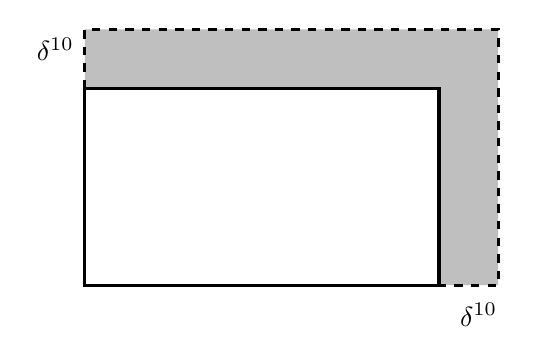
\begin{tikzpicture}[scale=0.5]
                %shaded area
                \draw[color=white,dashed,fill=white!75!black] (0,5)--(0,6.5)--(10.5,6.5)--(10.5,0)--(9,0)--(9,5)--cycle;
                  %Box
                \draw [very thick] (0,0) rectangle (9,5);
                %Dotted lines
                \draw[very thick, dashed] (0,5)--(0,6.5)--(10.5,6.5)--(10.5,0)--(9,0);
                \node at (-0.75, 6) {$\delta^{10}$};
                \node at (10, -0.75) {$\delta^{10}$};  
                %items
                \foreach \x/\y/\xx/\yy in {
                    0/0/1.5/1.5,
                    1.5/0/3.1/1.45,
                    3.1/0/4.5/1.43,
                    4.5/0/5.8/1.40,
                    5.8/0/7.2/1.38,                   
                    0/1.5/1.3/2.8,
                    1.3/1.5/2.5/2.75,
                    2.5/1.5/4/2.73,
                    4/1.5/6/2.7,
                    6/1.5/7.5/2.68,
                    7.5/1.5/9/2.67,
                    0/2.8/1.4/4.65,
                    1.4/2.8/2.7/4.63,
                    2.7/2.8/4.1/4.61,
                    4.1/2.8/5.5/4.58,
                    5.5/2.8/6.8/4.55,
                    6.8/2.8/8.2/4.5
                }
                {
					\drawGreenItem{\x}{\y}{\xx}{\yy};
				}
                %overlapping Items
                    \foreach \x/\y/\xx/\yy in {
                    7.2/0/9.1/1.35,
                    9.1/0/9.8/1.33,
                    8.2/2.8/9.5/4.45,
                    0/4.65/1.4/5.8,
                    1.4/4.65/2.6/5.78,
                    2.6/4.65/4.1/5.76,
                    4.1/4.65/5.3/5.74,
                    5.3/4.65/6.6/5.72,
                    6.6/4.65/7.3/5.6,
                    7.3/4.65/8.1/5.55,
                    8.1/4.65/9.1/5.52,
                    9.1/4.65/9.8/5.4
                }
                {
                    \drawYellowItem{\x}{\y}{\xx}{\yy};
                }                           
            \end{tikzpicture}
            \caption{Items overshooting the slot are shown as darker. These items can be repacked using \tNFDH.}
\label{fig:smallovershootrepack}
\end{figure}

The set $T_2$ consists of the wide, long and small items that overshoot their respective slots, together with all the small items that are packed in slots of width (resp. depth) smaller than $\delta^9$ inside the wide (resp. long) compartments. Consider first a (extended) slot for the wide items. Since the depth of the extension as well as the depth of any wide item are bounded by $\delta^{10}$, the total depth of the items not completely lying inside the original slot is at most $2\delta^{10}$. Since there are $O(1/\delta^6)$ such slots inside each configuration and the configurations have a total height not exceeding 1, the volume of the overshooting wide items is bounded by $2\delta^{10}\cdot O(1/\delta^6) = O(\delta^4)$. Analogously, the volume of the overshooting long items is also at most $O(\delta^4)$. Next consider a slot for small items. The total base area of the overshooting small items of any layer is at most $4\delta^{10}$ (see \Cref{fig:smallovershootrepack}). Thus their total volume is bounded by $4\delta^{10}\cdot O(1/\delta^5)=O(\delta^5)$. Finally, consider a slot of width (resp. depth) less than $\delta^9$ in which small items are packed inside a wide (resp. long) compartment. The total volume of all such slots is again bounded by $\delta^9\cdot O(1/\delta^5)=O(\delta^4)$. Hence we have $v(T_2)\le O(\delta^4)$ and are done.
%It is guaranteed in \cite{3d-strip-packing} that the total height of the layers used for packing the overshooting wide, long and small items is at most $O(\delta)$. Also, since there are $O(1/\delta^2)$ arrangements inside any wide/long compartment and a configuration contains at most $O(1/\delta^3)$ such compartments, the total volume of the remaining items of $T_2$ is bounded by $\delta^9 \cdot O(1/\delta^2) \cdot O(1/\delta^3) \le O(\delta^4)$, and hence they can be packed inside a box with $1\times 1$ base and height $O(\delta)$ using \texttt{3D-Vol-Pack}. 
%number of slots for wide, long and small items inside any configuration is bounded by $O(1/\delta^6)$.
%After the overshooting wide items have been repacked, the slots inside each arrangement are sorted from left to right in order of non-increasing packing depths, and the remaining free space inside the arrangement is partitioned into slots for packing the small items that were originally packed inside the wide compartment (see \cref{fig:space-small-items}). We focus on the packing inside one such slot. Similar to the case of the wide items, the width and depth of the slot are extended by $\delta^{10}$, and the small items are packed using \tNFDH~inside the extended slot. Again, the overshooting items are repacked into layers at the top. These overshooting small items are also items in $T_2$. The packing inside the long compartments is done in an analogous way. It is guaranteed in \cite{3d-strip-packing} that the total height of the layers used for packing the overshooting wide, long and small items is at most $O(\delta)$. Also, since there are $O(1/\delta^3)$ slots inside any wide/long compartment and a configuration contains at most $O(1/\delta^3)$ such compartments, the total number of slots for wide, long and small items inside any configuration is bounded by $O(1/\delta^6)$.
\end{proof}

% \begin{figure}[h]
%     \centering
%     \includesvg[width=\linewidth]{img/configurations-strip-removal.svg}
%     \caption{In Step 1, we delete at most $(1/3+O(\eps))$ fraction of the profit. In Step 2, we obtain a structured packing by \cite{3d-strip-packing}.}
%     \label{fig:configs-strip-removal}
% \end{figure}

Our objective is to build Area and Volume containers out of the slots for packing the wide/long and small items, respectively. The trouble is that the slot dimensions might not be large enough compared to the dimensions of the packed items, which is a necessary condition for the construction of such containers (see \Cref{sec:cont-class}). 
%In addition, the packing of $T_2$ might not be a container packing. 
We obtain a guessable container packing by the following lemma.
%(see \Cref{sec:omittedstrippacking} for a proof).

% \begin{restatable}{lemma}{roundingconfigTtwo}
% \label{lem:roundingconfigTtwo}
%     It is possible to repack the items of $T_2$ into a collection of $O(1/\delta^{12})$ guessable containers of total height at most $2\epsilon$.
% \end{restatable}


\begin{restatable}{lemma}{roundingconfigTone}
\label{lem:roundingconfigTone}
    By losing a profit of at most $\delta \opt_1$, and rounding the height of each configuration to the next integer multiple of $\mu/\epsilon$, each configuration for $T_1$ can be further partitioned into $O(1/\delta^6)$ guessable containers. Moreover, the items of $T_2$ can be packed inside a Steinberg container of height $\eps$.
\end{restatable}
\begin{proof}
We begin by discretizing the depths of the slots inside the wide compartments.

\begin{claim}
\label{lem:slotsandregions}
     By losing a profit of at most $O(\delta)\opt_1$, the depths of all the slots for wide and small items inside a wide compartment can be assumed to be a multiple of $\delta^9$.
\end{claim}
\begin{proof}
 We partition the compartment into strips each of depth $\delta^5$ and discard the minimum profitable strip, see \cref{fig:minStrip} for an illustration. Note that the depth of the compartment is a multiple of $\delta^4$, and hence the number of strips is at least $1/\delta$. Since each item has depth at most $\delta^{10}$, any item intersects at most two strips, and hence the total profit of the deleted items is at most an $O(\delta)$-fraction of the profit of the compartment. For any slot that is intersected by the deleted strip, we push the remaining items towards the front face of the slot, and notice that
 in the resulting packing, the wide and small items are packed using \NFDH (ignoring widths) and \tNFDH, respectively.

 \begin{figure}
    \centering
    \includesvg[width=0.7\linewidth]{img/deleted-strip-compartment.svg}
     % \begin{tikzpicture}[scale=0.5]
     %                %Box
     %                \draw[thick] (0,0)--(10,0)-- (10,10)--(0,10) -- (0,0);
     %                % Smaller strips
     %                %lowest
                    
     %                \foreach \x/\y/\xx/\yy in {
     %                    0/0/1.8/1.6,
     %                    1.8/0/3.4/1.57,
     %                    3.4/0/5.3/1.55,
     %                    5.3/0/7/1.54,
     %                    7/0/8.6/1.53,
     %                    8.6/0/9.9/1.52,
     %                    0/1.6/1.44/3.2,
     %                    1.44/1.6/2.72/3.17,
     %                    2.72/1.6/4.24/3.15,
     %                    4.24/1.6/5.6/3.14,
     %                    5.6/1.6/6.88/3.13,
     %                    6.88/1.6/7.92/3.12,
     %                    7.92/1.6/8.8/3.11,
     %                    8.8/1.6/9.68/3.1,
     %                    0/3.2/1.8/4.8,
     %                    1.8/3.2/3.4/4.77,
     %                    3.4/3.2/4.5/4.75,
     %                    4.5/3.2/6.2/4.74,
     %                    6.2/3.2/8/4.72,
     %                    8/3.2/9.5/4.71,
     %                    0/4.8/1.44/6.4,
     %                    1.44/4.8/2.72/6.37,
     %                    2.72/4.8/4.24/6.35,
     %                    4.24/4.8/5.6/6.34,
     %                    5.6/4.8/6.88/6.33,
     %                    6.88/4.8/7.92/6.32,
     %                    7.92/4.8/8.8/6.31,
     %                    8.8/4.8/9.68/6.3,
     %                    0/6.4/2.4/8,
     %                    2.4/6.4/4/7.97,
     %                    4/6.4/6.3/7.94,
     %                    6.3/6.4/8/7.92,
     %                    8/6.4/9.6/7.9,
     %                    0/8/1.5/9.6,
     %                    1.5/8/3.6/9.57,
     %                    3.6/8/5.7/9.55,
     %                    5.7/8/7.3/9.54,
     %                    7.3/8/8.4/9.53,
     %                    8.4/8/9.7/9.52
     %                }
     %                {
     %                \drawGreenItem{\x}{\y*0.2}{\xx}{\yy*0.2};
     %                }
     %                \foreach \x/\y/\xx/\yy in {
     %                    0/0/1.8/1.6,
     %                    1.8/0/3.4/1.57,
     %                    3.4/0/5.3/1.55,
     %                    5.3/0/7/1.54,
     %                    7/0/8.6/1.53,
     %                    8.6/0/9.9/1.52,
     %                    0/1.6/1.44/3.2,
     %                    1.44/1.6/2.72/3.17,
     %                    2.72/1.6/4.24/3.15,
     %                    4.24/1.6/5.6/3.14,
     %                    5.6/1.6/6.88/3.13,
     %                    6.88/1.6/7.92/3.12,
     %                    7.92/1.6/8.8/3.11,
     %                    8.8/1.6/9.68/3.1,
     %                    0/3.2/1.8/4.8,
     %                    1.8/3.2/3.4/4.77,
     %                    3.4/3.2/4.5/4.75,
     %                    4.5/3.2/6.2/4.74,
     %                    6.2/3.2/8/4.72,
     %                    8/3.2/9.5/4.71,
     %                    0/4.8/1.44/6.4,
     %                    1.44/4.8/2.72/6.37,
     %                    2.72/4.8/4.24/6.35,
     %                    4.24/4.8/5.6/6.34,
     %                    5.6/4.8/6.88/6.33,
     %                    6.88/4.8/7.92/6.32,
     %                    7.92/4.8/8.8/6.31,
     %                    8.8/4.8/9.68/6.3,
     %                    0/6.4/1.8/8,
     %                    1.8/6.4/3.4/7.97,
     %                    3.4/6.4/5.3/7.95,
     %                    5.3/6.4/7/7.94,
     %                    7/6.4/8.6/8,
     %                    8.6/6.4/9.9/8,
     %                    0/8/2.4/9.6,
     %                    2.4/8/4/9.57,
     %                    4/8/6.3/9.54,
     %                    6.3/8/8/9.52,
     %                    8/8/9.6/9.5
     %                }
     %                {
     %                \drawGreenItem{\x}{\y*0.2+1.92}{\xx}{\yy*0.2+1.92};
     %                }
     %                \foreach \x/\y/\xx/\yy in {
     %                    0/0/1.8/1.6,
     %                    1.8/0/3.4/1.57,
     %                    3.4/0/5.3/1.55,
     %                    5.3/0/7/1.54,
     %                    7/0/8.6/1.53,
     %                    8.6/0/9.9/1.52,
     %                    0/1.6/1.44/3.2,
     %                    1.44/1.6/2.72/3.17,
     %                    2.72/1.6/4.24/3.15,
     %                    4.24/1.6/5.6/3.14,
     %                    5.6/1.6/6.88/3.13,
     %                    6.88/1.6/7.92/3.12,
     %                    7.92/1.6/8.8/3.11,
     %                    8.8/1.6/9.68/3.1,
     %                    0/3.2/1.8/4.8,
     %                    1.8/3.2/3.4/4.77,
     %                    3.4/3.2/4.5/4.75,
     %                    4.5/3.2/6.2/4.74,
     %                    6.2/3.2/8/4.72,
     %                    8/3.2/9.5/4.71,
     %                    0/4.8/1.44/6.4,
     %                    1.44/4.8/2.72/6.37,
     %                    2.72/4.8/4.24/6.35,
     %                    4.24/4.8/5.6/6.34,
     %                    5.6/4.8/6.88/6.33,
     %                    6.88/4.8/7.92/6.32,
     %                    7.92/4.8/8.8/6.31,
     %                    8.8/4.8/9.68/6.3,
     %                    0/6.4/2.4/8,
     %                    2.4/6.4/4/7.97,
     %                    4/6.4/6.3/7.94,
     %                    6.3/6.4/8/7.92,
     %                    8/6.4/9.6/7.9,
     %                    0/8/1.4/9.6,
     %                    1.4/8/3.2/9.57,
     %                    3.2/8/5.7/9.55,
     %                    5.7/8/7.6/9.54,
     %                    7.6/8/8.8/9.53,
     %                    8.8/8/9.7/9.52
     %                }
     %                {
     %                \drawGreenItem{\x}{\y*0.2+3.84}{\xx}{\yy*0.2+3.84};
     %                }
     %                \foreach \x/\y/\xx/\yy in {
     %                    0/0/1.8/1.6,
     %                    1.8/0/3.4/1.57,
     %                    3.4/0/5.3/1.55,
     %                    5.3/0/7/1.54,
     %                    7/0/8.6/1.53,
     %                    8.6/0/9.9/1.52,
     %                    0/1.6/1.44/3.2,
     %                    1.44/1.6/2.72/3.17,
     %                    2.72/1.6/4.24/3.15,
     %                    4.24/1.6/5.6/3.14,
     %                    5.6/1.6/6.88/3.13,
     %                    6.88/1.6/7.92/3.12,
     %                    7.92/1.6/8.8/3.11,
     %                    8.8/1.6/9.68/3.1,
     %                    0/3.2/1.8/4.8,
     %                    1.8/3.2/3.4/4.77,
     %                    3.4/3.2/4.5/4.75,
     %                    4.5/3.2/6.2/4.74,
     %                    6.2/3.2/8/4.72,
     %                    8/3.2/9.5/4.71,
     %                    0/4.8/1.44/6.4,
     %                    1.44/4.8/2.72/6.37,
     %                    2.72/4.8/4.24/6.35,
     %                    4.24/4.8/5.6/6.34,
     %                    5.6/4.8/6.88/6.33,
     %                    6.88/4.8/7.92/6.32,
     %                    7.92/4.8/8.8/6.31,
     %                    8.8/4.8/9.68/6.3
     %                }
     %                {
     %                \drawGreenItem{\x}{\y*0.2+5.76}{\xx}{\yy*0.2+5.76};
     %                }                 
     %               \foreach \x/\y/\xx/\yy in {
     %                    0/6.4/1.8/8,
     %                    1.8/6.4/3.4/7.97,
     %                    3.4/6.4/5.3/7.95,
     %                    5.3/6.4/7/7.94,
     %                    7/6.4/8.6/8,
     %                    8.6/6.4/9.9/8,
     %                    0/8/2.4/9.6,
     %                    2.4/8/4/9.57,
     %                    4/8/6.3/9.54,
     %                    6.3/8/8/9.52,
     %                    8/8/9.6/9.5
     %                }
     %                {
     %                \drawGreenItem{\x}{\y*0.2+5.76}{\xx}{\yy*0.2+5.76};%-0.5
     %                }
     %                \foreach \x/\y/\xx/\yy in {
     %                    0/0/1.8/1.6,
     %                    1.8/0/3.4/1.57,
     %                    3.4/0/5.3/1.55,
     %                    5.3/0/7/1.54,
     %                    7/0/8.6/1.53,
     %                    8.6/0/9.9/1.52
     %                }
     %                {
     %                \drawGreenItem{\x}{\y*0.2+7.68}{\xx}{\yy*0.2+7.68};%-0.5
     %                }
     %                \foreach \x/\y/\xx/\yy in {
     %                    0/1.6/1.44/3.2,
     %                    1.44/1.6/2.72/3.17,
     %                    2.72/1.6/4.24/3.15,
     %                    4.24/1.6/5.6/3.14,
     %                    5.6/1.6/6.88/3.13,
     %                    6.88/1.6/7.92/3.12,
     %                    7.92/1.6/8.8/3.11,
     %                    8.8/1.6/9.68/3.1,
     %                    0/3.2/1.8/4.8,
     %                    1.8/3.2/3.4/4.77,
     %                    3.4/3.2/4.5/4.75,
     %                    4.5/3.2/6.2/4.74,
     %                    6.2/3.2/8/4.72,
     %                    8/3.2/9.5/4.71,
     %                    0/4.8/1.44/6.4,
     %                    1.44/4.8/2.72/6.37,
     %                    2.72/4.8/4.24/6.35,
     %                    4.24/4.8/5.6/6.34,
     %                    5.6/4.8/6.88/6.33,
     %                    6.88/4.8/7.92/6.32,
     %                    7.92/4.8/8.8/6.31,
     %                    8.8/4.8/9.68/6.3,
     %                    0/6.4/2.4/8,
     %                    2.4/6.4/4/7.97,
     %                    4/6.4/6.3/7.94,
     %                    6.3/6.4/8/7.92,
     %                    8/6.4/9.6/7.9,
     %                    0/8/1.5/9.6,
     %                    1.5/8/3.6/9.57,
     %                    3.6/8/5.7/9.55,
     %                    5.7/8/7.3/9.54,
     %                    7.3/8/8.4/9.53,
     %                    8.4/8/9.7/9.52
     %                }
     %                {
     %                \drawGreenItem{\x}{\y*0.2+7.68}{\xx}{\yy*0.2+7.68};
     %                }
     %                \foreach \x/\y/\xx/\yy in {
     %                    0/0/1.8/1.6,
     %                    1.8/0/3.4/1.57,
     %                    3.4/0/5.3/1.55,
     %                    5.3/0/7/1.54,
     %                    7/0/8.6/1.53,
     %                    8.6/0/9.9/1.52
     %                }
     %                {
     %                \drawGreenItem{\x}{\y*0.2+9.6}{\xx}{\yy*0.2+9.6};
     %                }

     %                \foreach \x in {
     %                1,2,3,4,5,6,7,8,9
     %                }
     %                {
     %                \draw[dashed] (0,\x) -- (10,\x);
     %                }
                    
     %                \draw[thick,decorate,decoration={brace,amplitude=5pt}] (-0.1,6) --(-0.1,7) node [midway, left = 8pt] {$\delta^5$};
     %                \draw[color=greenItem!60!white, pattern= north east lines, pattern color= greenItem!800!white] (0,3) rectangle (10,4);
     %                \draw[thick,decorate,decoration={brace,amplitude=5pt,mirror}] (10.1,3) --(10.1,4) node [midway, right = 8pt] {deleted strip};
     %                %\node at (-0.5,4.5) {$\delta^5$}
     %            \end{tikzpicture}   
    \caption{Rounding the depths of slots in a wide compartment. \kvnnew{The gray regions contain the small items.} All items intersecting the deleted strip are discarded.}
    \label{fig:minStrip}
\end{figure}
    
The resulting free space of depth $\delta^5$ inside the compartment will now be used to increase the depth of each arrangement. Specifically, we round up the depth of each arrangement (and hence each slot) to the next integral multiple of $\delta^9$. Since the total number of arrangements is $O(1/\delta^2)$, the total increase in depth is bounded by $O(\frac{1}{\delta^2})\cdot \delta^9 < \delta^5$.  
\end{proof}

In an analogous way, the widths of the slots inside long compartments can be made integral multiples of $\delta^9$. We next round up the heights of each of the configurations to integer multiples of $\mu/\epsilon$. Finally, we create the containers out of the configurations.

Recall that each configuration comprises $1/\delta^2$ compartments for big items, and $O(1/\delta^3)$ compartments for packing the wide, long, and small items. We create a Stack container corresponding to each of the compartments for the big items. The width (resp. depth) of this container is the same as the width (resp. depth) of some big item. Each wide compartment was further partitioned into $O(1/\delta^3)$ slots for packing the wide and small items. Note that due to \Cref{lem:slotsandregions}, the depth of a wide/small item is at most a $\delta$-fraction of the depth of the corresponding slot. Also, since we put the small items packed inside slots of width smaller than $\delta^9$ in the set $T_2$, the width of any small item in the set $T_1$ is at most a $\delta$-fraction of the width of the slot in which it is packed. Finally, the height of any configuration is at least $\mu/\epsilon$, which is at least an $1/\epsilon$-factor larger than the height of any item in $I_1$. We create an Area container corresponding to each slot for the wide items and a Volume container for each slot for the small items. The width of an Area container is the same as the width of some item in $I_1$. Also since the width of a wide compartment can have  $O(1/\delta^2)$ distinct values, and the width of a Volume container is either the same as the width of the wide compartment or equals the difference of the width of the compartment and the width of some slot (Area container), the width of a Volume container also lies in a polynomial-sized set. An analogous thing is done for the slots inside the long compartments. Finally, the heights of each of the  Stack, Area, and Volume containers are set to be the height of the configuration. Overall, we obtain $O(1/\delta^6)$ guessable containers corresponding to each configuration.

Since $T_2$ does not contain any big item and $v(T_2)\le O(\delta^4)$ by \Cref{lem:jansenpradelSP}, the conditions of \Cref{lem:steinberg} are trivially satisfied, and thus the whole set $T_2$ can be packed into a Steinberg container of height $\eps$.
\end{proof}






After applying the above lemma, the rounded heights of all the configurations for $T_1$ sum up to at most $(1-2\epsilon)+\frac{\mu}{\epsilon}\cdot O(\frac{1}{\delta^{6}}) \le 1-\eps$, for sufficiently small $\mu$. Since items of $T_2$ are packed inside a Steinberg container of height $\eps$, all the containers fit inside the knapsack and we obtain the following theorem overall.





% The algorithm of \cite{3d-strip-packing} repacks all the items into a set of $m = O(1/\delta^6)$ {\em configurations} and some additional layers at the top. We first describe the packing inside the configurations. Each such configuration $C$ is a cuboid of height $h_C$ with a square base of dimensions $1\times 1$ that is partitioned into at most $1/\delta^2$ {\em compartments} for big items, and at most $O(1/\delta^3)$ {\em compartments} for packing the wide, long, and small items (see \cref{fig:jp-configurations}).\footnote{Compartment is just a rectangular region.  In \cite{3d-strip-packing}, the term container was used to refer to compartment. In this work, we use compartment to avoid ambiguity.} Since the remaining items of $\text{OPT}\cap I_1$ were all packed within a height of at most $\frac{2}{3}-4\epsilon$ due to \Cref{lem:optspsmall}, the result of \cite{3d-strip-packing} implies that the sum of the heights of all the $m$ configurations is at most $\left(\frac{3}{2}+\epsilon\right)\left(\frac{2}{3}-4\epsilon\right)+\epsilon+
% f(1/\eps)\mu$, where $f$ is a function that is independent of $n$.  
% %frac{1}{\epsilon^{O(1/\epsilon)}}\mu 
% This is at most $1-3\epsilon$, for $\mu \le \eps / f(1/\eps)$ and sufficiently small $\epsilon$. 

 

%We round up the height of each configuration to the next integer multiple of $\mu/\delta^{2c}$, so that each configuration now has a height of at least $\mu/\delta^{2c}$. This increases the total height of the packing by at most $\frac{\mu}{\delta^{2c}} \cdot O(\frac{1}{\delta^6}) \le O(\epsilon)$ for sufficiently small $\mu$. 

% The big items are packed into their respective compartments by stacking them one on top of the other.
% %, thus creating a Stack container. Since the number of configurations is $O(1/\delta^6)$ and each configuration contains at most $1/\delta^2$ containers for big items, the number of Stack containers thus created is at most $O(1/\delta^8)$.} 
% We now describe the packing inside the wide compartments. The packing in the long compartments is analogous.



%\kvn{add caption}. The item depth dont seem to be atmost $\delta^{10}$. Need to change.



% Each wide compartment is divided into at most $O(1/\delta^2)$ \textit{arrangements}.\footnote{Again, in \cite{3d-strip-packing, jansen-pradel-bin-packing}, the term configuration was used instead of arrangement.} These arrangements are all possible multi-sets of wide items that have a total width of at most the width of the compartment (see \cref{fig:arrangements}). Since the width of any wide item is at least $\delta$, each arrangement consists of at most $1/\delta$ slots. %Inside any such slot, only those wide items are packed, whose rounded widths are exactly the same as the width of the slot. 
% To pack the wide items inside the slots, in the algorithm of \cite{3d-strip-packing}, first the depth of the slot is extended by $\delta^{10}$, and then the items are packed using \NFDH~inside the extended slot (see \Cref{fig:nfdhcrossing}). 
% Following this, the {\em overshooting} items of a particular slot that intersect the extended region are packed in a separate layer at the top. This may not be a container packing. We now show how to obtain a container packing of the {\em overshooting} items. Recall that the height of the slot is the same as the height of the corresponding configuration.

% \begin{restatable}{lemma}{wideovershoot}
% \label{lem:wideovershoot}
%     The overshooting wide items of any slot of height $h_C$ can be packed using \NFDH~inside a cuboidal region with $1\times 1$ base and height at most $O(\delta^{10})h_C +\mu$.
% \end{restatable}


% \ari{Each of these regions for packing the overshooting wide items will also be referred to as a \emph{configuration}.} After the overshooting items have been repacked, the slots inside each arrangement are sorted from left to right in order of non-increasing packing depths, and the remaining free space inside the arrangement is partitioned into rectangular regions for packing the small items that were originally packed inside the wide compartment (see \cref{fig:space-small-items}).


% We focus on the packing inside one such region. Similar to the case of the slots for wide items, the width and depth of the rectangular region are extended by $\delta^{10}$, and the small items are packed using 3D-\NFDH~inside the extended region. Again, the overshooting items are repacked into additional configurations using the following lemma.\mtr{Is the final figure I made meant to go here or in the appendix?}
% % \textcolor{red}{check:The small items are packed inside these regions using NFDH (note that the items in each layer are actually packed using Next-Fit-Decreasing-Depth). Again, the overshooting items are repacked into additional configurations using the following lemma.} 

% \begin{restatable}{lemma}{smallovershoot}
% \label{lem:smallovershoot}
%     The overshooting small items of any rectangular region of height $h_C$ can be repacked using \NFDH~inside a cuboid with $1\times 1$ base and height at most $O(\delta^{10})h_C + \mu$.
% \end{restatable}

% Next, note that, except possibly the rightmost rectangular region inside each arrangement, all the other regions have widths at least $\delta$. The rightmost rectangular region might not be usable as a Volume container if its width is not large enough compared to the small items
% packed in it. We consider each such region whose width is substantially small, and repack all the items packed inside the region into another configuration.

% \begin{restatable}{lemma}{smallrepack}
% \label{lem:smallrepack}
%     The small items that are packed inside the rightmost rectangular region (of an arrangement) that has width smaller than $\delta^{9}$, of a particular configuration having height $h_C$, can be repacked using \NFDH~inside a cuboid with $1\times 1$ base and height at most $O(\delta^{9})h_C+\mu$.
% \end{restatable}


% Recall that each initial configuration comprised $O(1/\delta^3)$ wide compartments, each containing $O(1/\delta^2)$ arrangements, each consisting of $1/\delta$ slots. Therefore the number of new configurations generated by Lemmas \ref{lem:wideovershoot}, \ref{lem:smallovershoot} and \ref{lem:smallrepack} is at most $O(1/\delta^6)$, and the height of each of these configurations is bounded by $O(\delta^{9})h_C+\mu$. Their total height is thus at most $O(\delta^{3})h_C + O(\mu/\delta^6) \le \epsilon h_C+O(\mu/\delta^6)$, for sufficiently small $\delta$. The increase in the height of the packing due to all these additional configurations is bounded by 
% $\epsilon\left(\frac{3}{2}+3\epsilon\right) + O\left(\frac{\mu}{\delta^6}\right)\cdot O\left(\frac{1}{\delta^6}\right) \le 2\epsilon$,
% for sufficiently small $\mu$.


% %Recall that each initial configuration comprised $O(1/\delta^3)$ wide compartments, each containing $O(1/\delta^2)$ arrangements, each consisting of $1/\delta$ slots. Therefore the number of new configurations generated by Lemmas \ref{lem:wideovershoot}, \ref{lem:smallovershoot} and \ref{lem:smallrepack} is at most $O(1/\delta^6)$, and the height of each of these configurations is bounded by $O(\delta^{c-1})h_C+\mu_s$. Their total height is thus at most $O(\delta^{c-7})h_C + O(\mu_s/\delta^6) \le \epsilon h_C+O(\mu_s/\delta^6)$, for sufficiently small $\delta$. The increase in the height of the packing due to all these additional configurations is bounded by 
% % $\epsilon\left(\frac{3}{2}+3\epsilon\right) + O\left(\frac{\mu_s}{\delta^6}\right)\cdot O\left(\frac{1}{\delta^6}\right) \le 2\epsilon$,
% % for sufficiently small $\mu_s$.

% \akr{add conditions for sufficiently small delta and mu}

% % %The number of new configurations generated due to the above lemma is at most $O(1/\delta^3)\cdot O(1/\delta^2) = O(1/\delta^5)$. We again round up the heights of these configurations to the nearest integral multiples of $\mu/\delta^{2c}$. Thus, the total (rounded) height of all the additional configurations corresponding to a configuration $C$ is bounded by 
% % \[ \left(O(\delta^c)h_C + \frac{\mu}{\delta^{2c}}\right)\cdot\frac{1}{\delta^6} + \left(O(\delta^{2c})h_C + \frac{\mu}{\delta^{2c}}\right)\cdot\frac{1}{\delta^6} + \left(O(\delta^{c-1})h_C + \frac{\mu}{\delta^{2c}}\right)\cdot \frac{1}{\delta^5} \le \epsilon h_C + O\left(\frac{1}{\delta^{2c+6}}\right)\mu \]
% % Thus, the total increase in the height of the packing due to the additional layers is at most $\epsilon(\frac{3}{2}+O(\epsilon))+O(1/\delta^{2c+6})\mu \cdot O(1/\delta^6) = O(\epsilon)$, for sufficiently small $\mu$.

% After applying Lemmas \ref{lem:wideovershoot}, \ref{lem:smallovershoot}, and \ref{lem:smallrepack}, we obtain a packing of a subset of wide and small items into containers (though their dimensions may not be from a polynomial-sized set). We now refine this packing to ensure that the container dimensions come from a \ari{set of size $n^{O(1/\delta^3)}$}. 

% \begin{restatable}{lemma}{slotsandregions}
% \label{lem:slotsandregions}
%     By losing an $O(\delta)$-fraction of the profit, the depths of all the slots for wide items and the rectangular regions for small items, can be assumed to be a multiple of $\delta^9$.
% \end{restatable}

% \ari{Analogously, we repack the long and small items inside the long compartments into such discretized slots and rectangular regions, respectively.} We note that the total number of configurations present in the current packing is $O(1/\delta^{12})$ -- there were $m=O(1/\delta^6)$ configurations to begin with, and for each initial configuration we created $O(1/\delta^6)$ additional configurations. We now round up the height of each configuration to the next integer multiple of $\mu/\epsilon$. This increases the total height by at most $\frac{\mu}{\epsilon}\cdot O\left(\frac{1}{\delta^{12}}\right) \le \epsilon$, for sufficiently small $\mu$. The resulting height of the packing is at most $(1-3\epsilon)+2\epsilon+\epsilon = 1$, and thus the packing fits inside the knapsack. Our final step is to build containers corresponding to the big compartments, slots and rectangular regions inside the configurations.

% \begin{lemma}
%     Each configuration can be partitioned into at most $O(1/\delta^6)$ guessable Stack, Area and Volume containers.
% \end{lemma}

% \akr{Use figure to show compartments, arrangements, slots, and rectangular region.}

% We now discretize the heights of these configurations.

% \akr{Use figure to show compartments, arrangements, slots, and rectangular region.}



% \begin{restatable}{lemma}{splitconfig}
% \label{lem:splitconfig}
%     Consider a configuration $C$ whose height $h_C > \epsilon^2$. Then by losing an $O(\epsilon)$-fraction of the profit, $C$ can be split into $O(1/\epsilon^3)$ configurations whose heights sum up to at most $h_C$, and each of whose heights is of the form $j\epsilon^4$, where $j\in [1/\epsilon]$.
% \end{restatable}


% For each configuration with height at most $\epsilon^2$, we round up the height to the next integer multiple of $\mu/\epsilon$. This increases the total height by at most $\frac{\mu}{\epsilon}\cdot O(\frac{1}{\delta^{12}}) \le \epsilon$, for sufficiently small $\mu$. The resulting height of the packing is at most $\left(\frac{3}{2}+3\epsilon\right)+2\epsilon+\epsilon = \frac{3}{2}+6\epsilon$.  We now discard some of the configurations\kvnr{removing configs may be probalematic. What if there is only one config? We should remove strips.} (see \cref{fig:strip-removal}), so that the remaining ones fit inside the knapsack. \deb{Also, we build containers corresponding to the big compartments, slots and rectangular regions inside the surviving configurations.}

% \begin{restatable}{lemma}{deleteonethird}
% \label{lem:deleteonethird}
%     There exists a packing of a subset of $OPT \cap I_1$ with profit at least $\left(\frac{2}{3}-O(\epsilon)\right)\opt_1$, into at most $(1/\epsilon \delta)^{O(1)}$ configurations inside the knapsack. \deb{Further, each configuration can be partitioned into at most $O(1/\delta^6)$ guessable Stack, Area and Volume containers.}
% \end{restatable}


%Recall that each configuration comprises $1/\delta^2$ compartments for big items, and $O(1/\delta^3)$ compartments for packing the wide, long, and small items. We create a Stack container corresponding to each of the compartments for the big items. The width (resp. depth) of this container is the same as the width (resp. depth) of some big item. Each wide compartment was further partitioned into $O(1/\delta^3)$ slots and rectangular regions, for packing the wide and small items, respectively. Note that due to \Cref{lem:slotsandregions}, the depth of a wide (resp. small) item is at most a $\delta$-fraction of the width of the slot (resp. rectangular region). Also, due to \Cref{lem:smallrepack}, the width of any small item is at most a $\delta$-fraction of the width of the region in which it is packed. Finally, the height of any configuration is at least $\text{min}\{\epsilon^4, \mu/\epsilon\} = \mu/\epsilon$, which is at least an $1/\epsilon$-factor larger than the height of any item in $I_1$. We create an Area container corresponding to each slot and a Volume container for each rectangular region for the small items. \ari{The width of an Area container is the same as the width of some item in $I_1$. Also since the width of a wide compartment can have  $O(1/\delta^2)$ distinct values, and the width of a Volume container is either the same as the width of the wide compartment or equals the difference of the width of the compartment and the width of some slot (Area container), the width of a Volume container also lies in a polynomial-sized set.} An analogous thing is done for the slots and regions inside the long compartments. Finally, the heights of each of the  Stack, Area, and Volume containers are set to be the height of the configuration. Overall, we obtain $O(1/\delta^6)$ containers corresponding to each configuration.
%\djr{One option is to mention in Lemma 14 that each config. can be divided into $O(1/\delta^6)$ guessable containers, and move this para to appendix.}

% The total number of containers in the knapsack is therefore bounded by $O(1/\delta^{12})\cdot O(1/\delta^6)=O(1/\delta^{18})$. The following theorem summarizes the structural result of this section.

\begin{theorem}
\label{thm:guessableconfig}
    %Consider the packing of $\text{OPT}\cap I_1$, having a profit of $\opt_1$. Then 
    We can repack a subset of $\text{OPT}\cap I_1$ with profit at least $\left(\frac{2}{3}-O(\epsilon)\right)\opt_1$ into \ari{$O(1/{\delta^{12}})$} guessable Stack, Area, and Volume containers. 
\end{theorem}

An equivalent restructuring of $\text{OPT}\cap I_2$ and $\text{OPT}\cap I_3$ gives the following corollary.

\begin{restatable}{corollary}{structuredpackingalgo}
\label{thm:structuredpackingalgo}
    $\optgs \ge \left(\frac{2}{3}-O(\epsilon)\right) \max\{\opt_1, \opt_2, \opt_3\}$.
\end{restatable}














% END AUTHOR FILE StripPacking.tex
% BEGIN AUTHOR FILE 5approx.tex

\subsection{A simple \texorpdfstring{$(5+\eps)$}{5+ε}-approximation}
\label{sec:5approx}
We now present a simple $(5+\epsilon)$-approximation for \tdk, which already improves upon the $(7+\epsilon)$-approximation \cite{3d-knapsack}. For this, first, we provide the following packing guarantee that will also be useful later.

\begin{lemma}
\label{lem:stackandsteincombine}
    Given a box $B$ whose base has dimensions $w_B\times d_B$ and height 1. Let $T$ be a set of items with $v(T)\le v(B)/4$ such that each $i\in T$ has $w_i \le w_B$, $d_i \le d_B$ and  $h_i\le \epsilon^4$. Let $T_{\ell} := \{i\in T \mid w_i > w_B/2 \text{ and } d_i > d_B/2\}$ and $T_s := T\setminus T_{\ell}$. Then it is possible to find a subset $T'_{\ell}\subseteq T_{\ell}$ with $p(T'_{\ell}) \ge (1-\epsilon)p(T_{\ell})$ and partition $B$ into a Stack and a Steinberg container by a horizontal plane parallel to the base, such that $T'_{\ell}$ and $T_s$ can be fully packed into the Stack and Steinberg containers, respectively. Furthermore, the heights of the two containers are integer multiples of $\epsilon^2$.
\end{lemma}
\begin{proof}
    To begin with, we create a Steinberg container having height $3(1+7\epsilon^2)\frac{v(T_s)}{w_Bd_B}+\epsilon^2$. Since $h_i \le \epsilon^4$, we have that the height of any item is at most an $\epsilon^2$-fraction of the height of the container. Clearly, the volume of the container is at least $3(1+7\epsilon^2)v(T_s)$. This implies that the whole set $T_s$ can be packed into the container since 
    \[ \left(\frac{1}{3}-2\epsilon^2\right)\cdot 3(1+7\epsilon^2)v(T_s) \ge v(T_s)\]
    for sufficiently small $\epsilon$. The height of the Steinberg container is then rounded up to the nearest integral multiple of $\epsilon^2$ - the resulting height is bounded by $\frac{3v(T_s)}{w_Bd_B}+O(\epsilon^2)$. In the remaining height of the box, we create a Stack container. Next, we sort the items of $T_{\ell}$ in non-increasing order of their profit to height ratio and pick a maximal prefix $T'_{\ell}$ that fits inside the Stack container. If $T'_{\ell} = T_{\ell}$, we already obtain a profit of $p(T_{\ell})$ and are done. Else, $h(T_{\ell})$ must be at least $1-\frac{3v(T_s)}{w_Bd_B}-O(\epsilon^2) \ge \frac{1}{5}$, since $v(T_s) \le v(B)/4$. Also, since the height of each item is bounded by $\epsilon^4$, we have 
    \begin{equation}
    \label{eqn:heightpacked}
        h(T'_{\ell}) \ge 1-\frac{3v(T_s)}{w_Bd_B}-O(\epsilon^2) - \epsilon^4 = 1-\frac{3v(T_s)}{w_Bd_B}-O(\epsilon^2).
    \end{equation}
    Now since $v(T) \le v(B)/4$, we have $\frac{1}{4}w_Bd_Bh(T_{\ell}) + v(T_s) \le \frac{1}{4}w_Bd_B$, and thus
    \begin{equation}
    \label{eqn:heightopt}
        h(T_{\ell}) \le 1 - \frac{4v(T_s)}{w_Bd_B}\le 1-\frac{3v(T_s)}{w_Bd_B}.
    \end{equation}
    From \eqref{eqn:heightpacked} and $\eqref{eqn:heightopt}$, we get $h(T'_{\ell}) \ge h(T_{\ell})-O(\epsilon^2) \ge (1-\epsilon)h(T_{\ell})$, since $h(T_{\ell})\ge 1/5$. Hence $p(T'_{\ell})\ge (1-\epsilon)p(T_{\ell})$ and we are done.   
    \kvnr{Low priority. Display math punctuation is not correct.}
\end{proof}

%\kvn{See \cref{sec:sec-3-2} for the proof.}

% \begin{restatable}{lemma}{onefourthvol}
% \label{lem:onefourthvol}
%     Let $T$ be a set of items such that each $i\in T$ satisfies $h_i \le \epsilon^4$. If $v(T) \le 1/4$, then there exists $T'\subseteq T$ with $p(T')\ge (1-\epsilon)p(T)$ such that there is a guessable container packing of $T'$ into a Stack and a Steinberg container.
% \end{restatable}

%Here we show that a combination of \Cref{lem:onefourthvol} and \Cref{thm:guessableconfig} already gives a $(5+\epsilon)$-approximation for \tdk, improving on the $(7+\epsilon)$-approximation of \cite{3d-knapsack}. 

Then the following lemma, together with \Cref{thm:ptasboxpacking}, gives a $(5+\epsilon)$-approximation.

\begin{lemma}
$\opt\le (5+\epsilon)\alg$.    
\end{lemma}
\begin{proof}
Trivially we have $\optgs \ge \opt_L$, since we can create a \kvnnew{Stack} container for every item in $\text{OPT}\cap L$ (at most $1/\mu^3$ such items). Hence if $\opt_L > \opt/5$, we are already done. Otherwise we have $\opt_1+\opt_2+\opt_3 \ge \frac{4}{5}\opt$. Now since $v_1 + v_2 + v_3 \le 1$, there must exist an $i \in [3]$ such that $\frac{\opt_i}{v_i} \ge \frac{4}{5}\opt$ -- w.l.o.g.~assume $i=1$. We have two cases.

%First, since $|\text{OPT}\cap L| \le 1/\mu^3$, we can enumerate all feasible choices of packing at most $1/\mu^3$ items of $L$ into the knapsack in $n^{O(1/\mu^3)}$ time. Choosing the most profitable among these will give us a profit of at least $\opt_L$. Hence if $\opt_L > \opt/5$, we are already done. Otherwise we have $\opt_1+\opt_2+\opt_3 \ge \frac{4}{5}\opt$. Now since $v_1 + v_2 + v_3 \le 1$, there must exist an $i \in [3]$ such that $\frac{\opt_i}{v_i} \ge \frac{4}{5}\opt$ -- w.l.o.g.~assume $i=1$. We consider two cases depending on the value of $v_1$.

\textbf{Case 1: $v_1 \le \frac{1}{4}$.} In this case, \Cref{lem:stackandsteincombine} (with the box $B$ corresponding to the whole knapsack) implies that $\optgs \ge (1-\epsilon)\opt_1$ (since each item in $I_1$ has height at most $\mu < \epsilon^4$). Hence if $\opt_1 > \opt/5$, we are done. Otherwise we have $\opt_2 + \opt_3 \ge \frac{3}{5}\opt$.  W.l.o.g.~ assume that $\opt_2 \ge \frac{3}{10}\opt$, \Cref{thm:structuredpackingalgo} gives us $\optgs \ge \left(\frac{2}{3}-O(\epsilon)\right)\cdot \frac{3}{10}\opt = \left(\frac{1}{5}-O(\epsilon)\right)\opt$.

%we apply the restructuring procedure of \Cref{sec:firstlb} to $\text{OPT}\cap I_2$ in order to obtain a guessable container packing having profit at least $\left(\frac{2}{3}-O(\epsilon)\right)\opt_2 \ge \left(\frac{1}{5}-O(\epsilon)\right)\opt$. Thus the packing returned by \Cref{thm:ptasboxpacking} will also have a profit of at least $\left(\frac{1}{5}-O(\epsilon)\right)\opt$, and we are done.

\textbf{Case 2: $v_1 > \frac{1}{4}$.} In this case, we sort the items of $\text{OPT}\cap I_1$ in non-increasing order of their profit to volume ratio, and pick the maximal prefix $T$ whose volume does not exceed $\frac{1}{4}$. Then we have $v(T) \ge \frac{1}{4}-\mu$. Applying \Cref{lem:stackandsteincombine} to $T$, we obtain
$\optgs \ge (1-\epsilon)\left(\frac{1/4-\mu}{v_1}\right)\opt_1 \ge \left(\frac{1}{5}-O(\epsilon)\right)\opt$,
thus completing the proof.
\end{proof}

%All these items can be packed into the knapsack using \Cref{lem:onefourthvol}. Since the volume of each item in $\text{OPT}\cap I_1$ is bounded by $\mu$, the volume packed is at least $\frac{1}{4} - \mu > \frac{1}{4}-3\epsilon$. Thus the profit obtaind is at least 
%\[ \frac{\frac{1}{4}-3\epsilon}{v_1}\opt_1 \ge \left(\frac{1}{5}-O(\epsilon)\right)\opt\]

\mt{The ratio of $(5+\eps)$ is tight. One such instance is given when $v_1 =\frac{1}{8}, v_2=v_3=\frac{3}{8} $ and $\opt_1=\opt_L=\frac{1}{5}\opt$ and $\opt_2=\opt_3=\frac{3}{10}\opt.$ }

We will obtain further improvements by using the lower bounds in the following sections.

% END AUTHOR FILE 5approx.tex
% BEGIN AUTHOR FILE BigLarge.tex

\subsection{Second lower bound on \texorpdfstring{$\optgs$}{optgs}}
\label{sec:secondlb}
In this subsection, we consider the packing of $\OPT\cap (I_{1\ell}\cup L)$, and restructure it to obtain a guessable container packing, by losing only an $O(\epsilon)$-fraction of the profit. 
Let $\OPTonel := \OPT\cap I_{1\ell}$ and $\OPTL := \OPT\cap L$. Since each item in $L$ has all side lengths at least $\hmax$, the number of such items in the packing is $|\OPTL| \le 1/\hmax^3$. 
% We create a Large container for each such item. 
Also, since the width and depth
of each item in $I_{1\ell}$ is at least 1/2, the items of $\OPTonel$ must be packed in layers, i.e., the top and bottom faces of any item in $\OPTonel$ when extended parallel to the bottom face of the knapsack will not intersect another item from $\OPTonel$. We now discretize the positions of the items in the packing.

\begin{restatable}{lemma}{discretepos}
\label{lem:discretepos}
    The distance of the left (resp. front) face of any item from the left (resp. front) face of the knapsack can be assumed to lie in a polynomial-sized set.
\end{restatable}
\begin{proof}
We push each item as much to the left as possible. Then for each item in $\OPTonel$, the distance of its left face (from the left face of the knapsack) can be written as the sum of the widths of at most $1/\hmax$ items from $L$. Similarly, the distance of the left face of any item in $\OPTL$ is the sum of the widths of at most $1/\hmax$ items of $L$ and at most one item from $\OPTonel$. Analogous claims hold by pushing the items as much to the front as possible.
\end{proof}


\begin{figure}
    \centering
    \includesvg[width=0.7\linewidth]{img/number-theory-1.svg}
    \caption{Packing of items in $OPT \cap (L\cup I_{1\ell})$: The dotted (resp. dashed) lines show (front view of) horizontal planes passing through the top and bottom faces of items in $\OPTL$ (resp.  $T$). We discard the items in $\OPTonel \setminus T$ that are cut by these planes.}
    \label{fig:Planes cutting}
\end{figure}

Let $T\subseteq \OPTonel$ be the $k$ items of largest profit in $\OPTonel$, for some $k$ to be chosen later. Our goal is to obtain a container packing of all items in $\OPTL$, together with a subset of $\OPTonel$ having a profit of at least $(1-\epsilon)\optonel$. To this end, we shall pack all items in $T$ and ensure that the number of discarded items of $\OPTonel$ is bounded by $ck$, for some constant $c$. By a result of \cite{jansen1999improved}, the profit of the discarded items can be bounded by $\epsilon \optonel$, for appropriately chosen $k$. We now outline the details of our restructuring procedure. See \cref{fig:Planes cutting}.

We draw horizontal planes passing through the top and bottom faces of the items in $T\cup \OPTL$, and discard the items of $\OPTonel \setminus T$  intersecting these planes (see \cref{fig:Planes cutting}). The number of discarded items is bounded by $2|\OPTL|=O(1/\mu^3)$. The remaining items of $\OPTonel\setminus T$ are now completely packed inside at most $k+2|\OPTL|+1$ horizontal strips demarcated by the planes. Each such strip is a cuboidal box that is pierced from top to bottom by at most $1/\hmax^2$ Large \kvnnew{items}. Further, there are only polynomially-many positions of these Large \kvnnew{items} inside the strip owing to \Cref{lem:discretepos}. We focus on one such strip $\SM$.

%Next, we create a Stack container for every item in $T$, having dimensions same as those of the item. 
% \begin{figure}
%         \centering
%         \begin{minipage}{0.45\textwidth}
%             \centering
%             \begin{tikzpicture}[scale=0.8]
%             %Light Blue
% 				\drawLightBlueCuboidDashed{0}{1.1}{0}{6}{0.2}{6};
% 				\drawLightBlueCuboidDashed{0}{1.7}{0}{6}{0.2}{6};
% 				\drawLightBlueCuboidDashed{0}{3.4}{0}{6}{0.2}{6};
% 				\drawLightBlueCuboidDashed{0}{3.9}{0}{6}{0.2}{6};
% 				%Red
% 				\drawRedCuboidDashed{3}{0}{0}{2}{1}{3};
% 				\drawRedCuboidDashed{0}{1.9}{3}{1.5}{1.5}{2.5};
% 				\drawRedCuboidDashed{0.5}{4.1}{2}{1.5}{1.9}{2.5};
% 				%Green
% 				\drawGreenCuboidDashed{1}{1.3}{2}{3}{0.3}{2.5};
% 				\drawGreenCuboidDashed{2.5}{3.6}{0}{3}{0.3}{2.5};
% 				%Box
% 				\drawBlackCuboidDashed{0}{0}{0}{6}{6}{6};
% 			\end{tikzpicture} 
%         \end{minipage}\hfill
%         \begin{minipage}{0.45\textwidth} 
%             \centering            
% 				\begin{tikzpicture}
% 				\draw (0,0) rectangle (6,6);
% 				%Red
% 				\draw [color=redItem!80!black, pattern=north west lines, pattern color=redItem!80!black] (3,0) rectangle (5,1.1);
% 				\draw [color=redItem!80!black, pattern=north west lines, pattern color=redItem!80!black] (0,1.8) rectangle (1.5,3.4);
% 				\draw [color=redItem!80!black, pattern=north west lines, pattern color=redItem!80!black] (0.5,4.1) rectangle (2,6);
% 				%LB
% 				\draw [formerLB, pattern=north east lines, pattern color= formerLB] (0,1.1) rectangle (6,1.3);
% 				\draw [color=formerLB, pattern=north east lines, pattern color=formerLB] (0,1.6) rectangle (6,1.8);
% 				\draw [color=formerLB, pattern=north east lines, pattern color=formerLB] (0,3.4) rectangle (6,3.6);
% 				\draw [color=formerLB, pattern=north east lines, pattern color=formerLB] (0,3.9) rectangle (6,4.1);
% 				%Green
% 				\draw [color=greenItem!75!black, pattern=crosshatch, pattern color=greenItem!75!black] (1,1.3) rectangle (4,1.6);
% 			\end{tikzpicture}
			
%         \end{minipage}
%         \caption{Planes formed after extending the top and bottom faces of items in $T\cup T_2$.}
%         \label{fig:Planes cutting}
%     \end{figure}
%Next, we discard the at most $2|T_2|$ items of $T_1$ that are intersected by these planes. The remaining items of $T_1$ are now completely packed inside the at most $2(k+|T_2|)+1$ horizontal strips thus created. Barring $k$ strips which contain a single item from $T$, each of the remaining strips is a cuboidal region that is pierced from top to bottom by at most $1/\hmax^2$ Large containers. Further, there are only polynomially-many positions of these Large containers inside the strip owing to \Cref{lem:discretepos}. We focus on one such strip $\SM$.

\begin{restatable}{lemma}{boundingStackcontainer}
\label{lem:boundingStackcontainer}
    The items of $\OPTonel \setminus T$ present inside the strip $\SM$ can be repacked into at most $O(1/\mu^8)$ Stack containers, whose widths and depths lie in a polynomial-sized set.
\end{restatable}
\begin{proof}
Consider the top face of the strip $\SM$. We extend the boundary edges of the at most $1/\mu^2$ Large \kvnnew{items}, till they hit the boundary of another Large \kvnnew{item} or the boundary of the knapsack. Consider all the rectangular regions formed by these lines. We call a region to be \textit{maximal} if it does not contain any Large \kvnnew{item}, and is not completely contained inside a larger region (see \cref{fig:maximal-regions}).
%\kvnrnew{Where are big items in the caption defined?}
    \begin{figure}
        \centering
   %      \begin{tikzpicture}[scale=0.4]
   %              \draw[fill=white!80!black, opacity=0.6] (3.5,3) rectangle (6,6.5);
   %              \draw[fill=white!80!black, opacity=0.6] (3.5,7.75) rectangle (6,10);
			% 	%Filled Boxes
			% 	\drawGreenFilledArea{3.5}{7.75}{10}{10};
			% 	\drawGreenFilledArea{3.5}{3}{6}{7.75};
			% 	\drawGreenFilledArea{0}{3}{3.5}{6.5};
			% 	%\drawGreenFilledArea{6.5}{0}{10}{3.75};
   %              %darker shaded Crossovers
                
                
                
			% 	%Items
			% 	\drawYellowItem{6.04}{3.79}{8.96}{7.71};
			% 	\drawYellowItem{1.54}{1.04}{6.46}{2.96};
			% 	\drawYellowItem{1.04}{6.54}{3.46}{8.96};
			% 	%Grey Lines
			% 	%1st item (lowest)
			% 	\draw[color=black!45!white, very thick] (0,1)--(10,1);
			% 	\draw[color=black!45!white, very thick] (0,3)--(10,3);
			% 	\draw[color=black!45!white, very thick] (1.5,0)--(1.5,6.5);
   %              \draw[color=black!45!white, very thick](6.5,0)--(6.5,3.75);
			% 	%2nd item
			% 	\draw[color=black!45!white, very thick] (6,3)--(6,10);
			% 	\draw[color=black!45!white, very thick] (0,3.75)--(10,3.75);
			% 	\draw[color=black!45!white, very thick] (9,0)--(9,10);
			% 	%3rd item
			% 	\draw[color=black!45!white, very thick] (0,9)--(10,9);
			% 	\draw[color=black!45!white, very thick] (0,6.5)--(6,6.5);
   %              \draw[color=black!45!white, very thick] (1,0)--(1,10);
   %              %Highlighed Area
   %              \draw[color=black!85!white,very thick] (3.5,7.75) rectangle (10,10);
   %              %node
   %              \node (text) at (15,8.75) {Maximal Region};
   %              %arrow
   %              \draw[-stealth] (text) -- (10.1,8.75);
			% 	%Box
			% 	\draw[very thick] (0,0)--(10,0)-- (10,10)--(0,10) -- (0,0);
			% \end{tikzpicture}
        \includesvg[width=0.7\linewidth]{img/maximal-regions}
        \caption{\kvn{Maximal regions. Left: Strip between two consecutive planes. Large items (hatched) span the entire height of the strip. Right: Top view of the strip.}}
        \label{fig:maximal-regions}
    \end{figure}
    
    % \akr{add a proper figure with one strip and corresponding regions}
    
    Then note that the top face of each item of $\OPTonel$ that is packed inside $\SM$ must lie completely inside at least one of these maximal regions, and we assign the item to one of these regions arbitrarily. Afterward, we permute the items of $\OPTonel$ so that all items assigned to a particular maximal region are stacked consecutively one above the other. Hence, for each maximal region, we obtain a Stack container containing all items of $\OPTonel$ assigned to it, whose width and depth are the same as those of the region. Since there were at most $1/\mu^2$ Large \kvnnew{items} to begin with, the number of maximal regions and therefore the number of Stack containers obtained is bounded by $O((1/\mu^2)^4) = O(1/\mu^8)$. Also, from \Cref{lem:discretepos}, the possible locations of the Large \kvnnew{items} were polynomially many, and thus there is only a polynomial number of choices for the widths and depths of the Stack containers.
\end{proof}


For each item in \kvnnew{$T\cup \OPTL$}, we create a Stack container containing the single item itself. Together with \Cref{lem:boundingStackcontainer}, we get a constant number of Stack containers inside the knapsack. We now discretize the heights of the Stack containers, so that they lie in a polynomial-sized set.

\begin{restatable}{lemma}{discard}
\label{lem:discard}
    By discarding $O(1/\mu^{11})k$ items from $\OPTonel\setminus T$, the height of each Stack container can be made of the form $j\Bar{h}$, where $j\in [n]$ and $\Bar{h}$ is the height of some item in \kvnnew{$I_{1\ell}\cup L$}.
\end{restatable}
\begin{proof}
If a Stack container contains a single item, we make the height of the container equal to the height of that item. Consider now a Stack container having at least two items of $I_{1\ell}$. Let $\Bar{h}$ be the height of an item with the second largest height. We discard the item with the largest height and use the resulting empty space to round down the height of the container to the nearest integer multiple of $\Bar{h}$. Since the number of items packed inside the container is bounded by $n$, the rounded height of the container cannot exceed $n\Bar{h}$. Finally, since the number of Stack containers inside any strip is $O(1/\mu^8)$ (\Cref{lem:boundingStackcontainer}) and there are at most $k+2|\OPTL|+1 \le O(1/\mu^3)k$ strips, the total number of discarded items is bounded by $O(1/\mu^{11})k$.
\end{proof}


Together with the $O(1/\mu^3)$ items that were discarded previously, \Cref{lem:discard} gives us that the total number of discarded items so far is at most $O(1/\mu^{11})k$. We now use the following lemma from \cite{jansen1999improved}.
\begin{lemma}[\cite{jansen1999improved}]
    Let $p_1\ge p_2\ge \ldots \ge p_n>0$ be a sequence of real numbers and $P=\sum_{i=1}^{n} p_i$. Let $c$ be a nonnegative integer and $\epsilon >0$. If $n = c^{\Omega(1/\epsilon)}$, then there is an integer $k \le c^{O(1/\epsilon)}$ such that $p_{k+1}+\ldots p_{k+ck} \le \epsilon P$.
    
\end{lemma}


The above lemma invoked with $c=O(1/\hmax^{11})$ and with the correct guess of $k$ gives us that the total profit of the discarded items is at most $\epsilon \optonel$, assuming that $|\OPTonel|$ was sufficiently large (at least $n_0 := (1/\mu)^{\Omega(1/\epsilon)}$) to begin with. Otherwise, if $|\OPTonel| \le n_0$, we can create a separate Stack container for each item in $\OPTonel$ having dimensions same as that of the item, which together with the Stack containers for items in $\OPTL$ directly yields a guessable container packing of profit $\opt_L + \optonel$. The following theorem summarizes the arguments of this section.

\begin{restatable}{theorem}{ptasforcombine}
    Consider the packing of $\OPT\cap (I_{1\ell}\cup L)$.
    %and assume that there are at least $n_0 = (1/\mu)^{\Omega(1/\epsilon)}$ items in $\OPT\cap I_{1\ell}$. 
    Then by discarding items of $\OPT\cap I_{1\ell}$ having a total profit of at most $\epsilon\optonel$, the remaining items can be repacked into a guessable container packing, wherein items of $L$ are placed inside at most $1/\hmax^3$ \kvnnew{Stack} containers, and items of $I_{1\ell}$ are packed into at most $(1/\mu)^{O(1/\epsilon)}$ Stack containers.
\end{restatable}


%\akr{remove corollary and other details}

%If $\OPT\cap I_{1\ell}$ had less than $n_0$ items, to begin with, we create a separate Stack container for each such item, having dimensions same as those of the item, thus obtaining a container packing. Analogous restructuring of the packings $\OPT\cap (I_{2\ell}\cup L)$ and $\OPT\cap (I_{3\ell}\cup L)$ gives the following corollary.


% END AUTHOR FILE BigLarge.tex
% BEGIN AUTHOR FILE VolumeI1.tex

\subsection{Third lower bound on \texorpdfstring{$\optgs$}{optgs}}
\label{sec:thirdlb}

%In this subsection and the next subsection, using Steinberg's algorithm for 2D packing, we obtain improved bounds for volumes of packed items in 3D. 


In this subsection, we restructure the packing of items in $\text{OPT}\cap I_1$. Recall that $\optonel = p(\text{OPT}\cap I_{1\ell})$ and $\optones = p(\text{OPT}\cap I_{1s})$, so that $\optonel+\optones = \opt_1$. Also, $v_1 := v(\text{OPT}\cap I_1)$ and $\vones = v(\text{OPT}\cap I_{1s})$. 



%See \Cref{sec:packI1andcombine} for a proof of the following theorem.

%$\honel = h(\text{OPT}\cap I_{1\ell})$ and $\vones = v(\text{OPT}\cap I_{1s})$. Also $\optonel = p(\text{OPT}\cap I_{1\ell})$ and $\optones = p(\text{OPT}\cap I_{1s})$, so that $\optonel+\optones = \opt_1$. Finally, $v_1 := v(\text{OPT}\cap I_1)$. See \Cref{sec:packI1andcombine} for a proof of the following theorem.


% First, we state the following results from \cite{li1990three} that we repeatedly use in this and the following sections.

% \begin{lemma}[\cite{li1990three}]
% \label{thm:li-cheng}
% The following statements hold.
%     \begin{enumerate}
%         \item Let $T\subseteq I_{1s}$. Then the items in $T$ can be packed inside an LC\textsuperscript{a} container with $1\times 1$ base and having a height of $3v(T)+8\mu_s$.
%         \item Let $T\subseteq I_1$ and $\AM$ be a rectangular region such that the base of each item in $T$ fits inside $\AM$. Then the items in $T$ can be packed into an LC\textsuperscript{b} container with base $\AM$ and having a height of $4v(T)/\text{area}(\AM)+8\mu_s$.
%     \end{enumerate}
% \end{lemma}

% We are now ready to state the main structural result of this section.

\begin{restatable}{theorem}{packingI}
\label{thm:packingI1}
    Consider the packing of $\text{OPT}\cap I_1$. It is possible to repack subsets of $\text{OPT}\cap I_{1\ell}$ and $\text{OPT}\cap I_{1s}$ into a guessable Stack and Steinberg container, respectively, whose profit, say $P$, satisfies the following properties.
    \begin{itemize}
        \item $\displaystyle P \ge (1-O(\epsilon))\frac{\opt_{1s}}{\max\{3\vones, 1\}}$.
        \item If $v_1\le 1/3$, then $\displaystyle P  \ge (1-O(\epsilon))\left(\frac{3}{4}\optonel+\optones\right)$.
        \item If $v_1 \le 1/4$, then $P\ge (1-O(\epsilon))\opt_1$.
    \end{itemize}
    
    % \begin{enumerate}
    %     \item The following statements hold for the profit, say $P$, of the packed items.
    %     \begin{itemize}
    %         \item If $\vones>1/3$, then $P \ge (1-O(\epsilon))\frac{\optones}{3\vones}$.
    %         \item If $\vones \le 1/3$, then $P \ge (1-O(\epsilon))\optones$.
    %         %\item If $v_1>1/3$, then $P \ge (1-O(\epsilon))\alpha_2/3$.
    %         \item If $v_1\le 1/3$, then $P  \ge (1-O(\epsilon))\left(\frac{3}{4}\optonel+\optones\right)$.
    %         \item If $v_1 \le 1/4$, then $P\ge (1-O(\epsilon))\opt_1$.
    %     \end{itemize}
    %     \item Both the Stack and Steinberg containers have an $1\times 1$ base, and their heights are integral multiples of $\epsilon^2$.
        %\item The height of the LC\textsuperscript{a} container is an integral multiple of $\epsilon^2$.
    %\end{enumerate}
\end{restatable}
%\akr{condensify the theorem. $\min(1,1/4v_1)opt_{1l}+opt_{1s}$}

In order to prove the above, we first establish the following lemma that will also be used in the next subsection.

\begin{lemma}
\label{lem:stackandstein}
    The following statements hold.
    \begin{enumerate}
        \item If $v_1 \in (2\epsilon, 1/3]$, it is possible to obtain a container packing of a subset $T \subseteq \text{OPT}\cap I_1$ with $p(T) \ge (1-O(\epsilon))\left(\frac{3}{4}\optonel + \optones\right)$, such that the items of $T\cap I_{1\ell}$ and $T\cap I_{1s}$ are packed into a Stack and a Steinberg container, respectively. Both the containers have an $1\times 1$ base and further, their heights are integer multiples of $\epsilon^2$ and they sum to at most $3v_1$.
        \item If $v_1 \le 2\epsilon$, the items of $\text{OPT}\cap I_{1\ell}$ and $\text{OPT}\cap I_{1s}$ can be packed into a Stack and a Steinberg container respectively, both of whose bases have dimensions $1\times 1$, and whose heights are $8\epsilon$ each.
    \end{enumerate}    
\end{lemma}
\begin{proof}
    We first give a proof of the second case, which is much simpler. Since $v_1\le 2\epsilon$, we must have $\honel\le 8\epsilon$, and therefore the items of $\text{OPT}\cap I_{1\ell}$ can be packed into a Stack container with $1\times 1$ base and height $8\epsilon$. Similarly, the items of $\text{OPT}\cap I_{1s}$ can be packed into a Steinberg container with $1\times 1$ base and height $8\epsilon$ using \Cref{lem:steinberg}, since $\mu \le \epsilon\cdot 8\epsilon$ and $\left(\frac{1}{3}-2\epsilon\right)8\epsilon > 2\epsilon \ge \vones$.


    For the first case, we further subdivide the proof into two cases depending on the relative values of $v_1$ and $\vones$.

    \textbf{Case 1 : $v_1-\vones >\epsilon$.} In this case, we first create a Steinberg container $C$ with $1\times 1$ base and height $3(1+7\epsilon^2)\vones + \epsilon^2$. Note that the height of any item $i\in \text{OPT}\cap I_{1s}$ satisfies $h_i \le \mu < \epsilon^4 \le \epsilon^2 h_C$. We show that $\vones \le \left(\frac{1}{3}-2\epsilon^2\right)v(C)$, which implies that the items of $\text{OPT}\cap I_{1s}$ can be fully packed into the container $C$ by \Cref{lem:steinberg}. We have
    \[ \left(\frac{1}{3}-2\epsilon^2\right)v(C) \ge (1-6\epsilon^2)(1+7\epsilon^2)\vones
    > \vones, \]
    for sufficiently small $\epsilon$. We now round up the height of $C$ to the next multiple of $\epsilon^2$. The resulting value of $h_C$ is at most $3\vones+ 9\epsilon^2$. Note that since all items of $\text{OPT}\cap I_{1s}$ are packed, we obtain the full profit of $\optones$ from them. Next, we sort items in $\text{OPT}\cap I_{1\ell}$ in non-increasing order of profit to height ratio, and pick a maximal prefix whose height does not exceed $\epsilon^2 \lfloor3v_1/\epsilon^2\rfloor -h_C$ and pack them into a Stack container of the same height and with an $1\times 1$ base. Note that the height of the Stack container is also an integer multiple of $\epsilon^2$. If we are able to pack all items of $\text{OPT}\cap I_{1\ell}$, we obtain a profit of $\optonel$, and are done. Otherwise, the height of the packed items is at least $3v_1-\epsilon^2 - h_C -\mu\ge 3v_1-3\vones-11\epsilon^2 \ge (1-4\epsilon)(3v_1 - 3\vones)$. The profit obtained from $\text{OPT}\cap I_{1\ell}$ is then at least
    \[ \frac{(1-4\epsilon)(3v_1-3\vones)}{\honel}\optonel \ge \left(\frac{3}{4}-O(\epsilon)\right)\optonel, \]
    where the last inequality follows from the fact that $v_1\ge \frac{1}{4}\honel+\vones$.

    \textbf{Case 2 : $v_1 - \vones \le \epsilon$.} Since $v_1 > 2\epsilon$, it follows that $\vones > \epsilon$ in this case. We group the items of $\text{OPT}\cap I_{1s}$ into maximal groups of volume at most $8\epsilon^2$ each. Since $\vones > \epsilon$, the number of groups is at least $\Omega(1/\epsilon)$ and each group (except possibly one) has a volume of at least $8\epsilon^2-\mu>7\epsilon^2\ge 7\epsilon^2 \vones$. We delete the group having minimum profit. The remaining items have a volume of at most $(1-7\epsilon^2)\vones$ and a profit of at least $(1-O(\epsilon))\optones$. We claim that all these items can be packed into a Steinberg container $C$ having an $1\times 1$ base and height $3\vones-3\epsilon^2$. First note that since $\vones >\epsilon$, $h_C >\epsilon$ and therefore, for any $i\in \text{OPT}\cap I_{1s}$, we have $h_i \le \mu < \epsilon^3 \le \epsilon^2 h_C$. Also
    \[ \left(\frac{1}{3}-2\epsilon^2\right)v(C) \ge (1-6\epsilon^2)(1-\epsilon^2)\vones > (1-7\epsilon^2)\vones\]
    and thus the claim follows using \Cref{lem:steinberg}. We round up the height of the Steinberg container $C$ to the nearest integer multiple of $\epsilon^2$. Next, we create a Stack container of $1\times 1$ base, and having a height such that the sum of the heights of the two containers is exactly $\epsilon^2\lfloor 3v_1/\epsilon^2\rfloor$. This directly ensures that the height of the Stack container is a multiple of $\epsilon^2$. Also note that the height is at least $3v_1-3\vones + \epsilon^2$. We sort the items of $\text{OPT}\cap I_{1\ell}$ in non-increasing order of their profit to height ratio and pick a maximal prefix that has height at most $3v_1-3\vones+\epsilon^2$, which we pack in layers inside the Stack container. If, by doing this, we are able to pack all items of $\text{OPT}\cap I_{1\ell}$, we already obtain a profit of $\optonel$, and are done. Else the total height of the packed items is at least $3v_1-3\vones+\epsilon^2-\mu > 3v_1-3\vones$. Hence, the profit obtained from items of $\text{OPT}\cap I_{1\ell}$ is at least $\frac{3v_1-3\vones}{\honel}\optonel \ge \frac{3}{4}\optonel$, and we are done.
\end{proof}

We are now ready to prove \Cref{thm:packingI1}.

\begin{proof}[Proof of \Cref{thm:packingI1}]
     For the first bound, we sort the items of $\text{OPT}\cap I_{1s}$ in non-increasing order of their profit to volume ratio. We then pick the maximal prefix whose volume does not exceed $\frac{1}{3}-2\epsilon$. Using \Cref{lem:steinberg}, these items can be packed into a Steinberg container of dimensions same as those of the knapsack. We now analyze the profit of this packing. If all items of $\text{OPT}\cap I_{1s}$ are packed, we trivially obtain a profit of $\optones$ from them, and are done. Otherwise, since the volume of each item of $I_{1s}$ is at most $\mu$, the total volume of packed items is at least $\frac{1}{3}- 2\epsilon -\mu > \frac{1}{3}-3\epsilon$. Hence, the profit obtained is at least 
    \[ \frac{\frac{1}{3}-3\epsilon}{\vones}\optones \ge (1-O(\epsilon))\frac{\optones}{3\vones}\]
    and we get the desired guarantee in the first case. 

    The proof of the second and third cases directly follows from \Cref{lem:stackandstein} and \Cref{lem:stackandsteincombine}, respectively.
\end{proof}

  
















\iffalse
\begin{proof}[Proof of \Cref{thm:packingI1}]
    For the first two cases, we sort the items of $\text{OPT}\cap I_{1s}$ in non-increasing order of their profit to volume ratio. We then pick the maximal prefix whose volume does not exceed $\frac{1}{3}-2\mu_s$. Using \Cref{lem:steinberg} (with $\epsilon$ replaced by $\mu_s$), these items can be packed into a Steinberg container of dimensions same as those of the knapsack. We now analyse the profit of this packing. If all items of $\text{OPT}\cap I_{1s}$ are packed, we trivially obtain a profit of $\alpha_2$ from them, and are done. Otherwise, since the volume of each item of $I_{1s}$ is at most $\mu_s$, the total volume of packed items is at least $\frac{1}{3}-3\mu_s$. Hence, the profit obtained is at least 
    \[ \frac{\frac{1}{3}-3\mu_s}{x_2}\alpha_2 \ge (1-O(\epsilon))\frac{\alpha_2}{3x_2}\]
    and we get the desired guarantee in the first case. For the second case. the result directly follows using the fact that $x_2 \le 1$.
    
    
    Next we consider the case when $v_1\le 1/3$. Also, we assume for now that $x_2 > 1/4$. We group the items of $\text{OPT}\cap I_{1s}$ into maximal groups of volume at most $8\epsilon$ each. Since $x_2 > 1/4$, the number of groups is at least $\Omega(1/\epsilon)$ and each group (except possibly one) has a volume of at least $8\epsilon-\mu_s>7\epsilon\ge 7\epsilon x_2$. We delete the group having minimum profit. The remaining items have a volume of at most $(1-7\epsilon)x_2$ and a profit of at least $(1-O(\epsilon))\alpha_2$. We show that all these items can be packed into a Steinberg container of height $3x_2-2\epsilon^2$.
    
    \begin{claim}
        Let $T\subseteq I_{1s}$ such that $v(T)\le (1-7\epsilon)x_2$. If $x_2 > \epsilon$, then the whole set $T$ can be packed into a Steinberg container with $1\times 1$ base and height $3x_2-2\epsilon^2$.
    \end{claim}
    \begin{proof}
        Note that since $T\subseteq I_{1s}$ and the base of the Steinberg container has dimensions $1\times 1$, we directly have that either $w_i \le w_C/2$ or $d_i \le d_C/2$ holds. By \Cref{lem:steinberg}, it suffices to show that $v(T)\le \left(\frac{1}{3}-2\epsilon\right)v(C)$. Note that $v(C) = 3x_2 - 2\epsilon^2 \ge 3(1-\epsilon)x_2$. Thus
        \[ \left(\frac{1}{3}-2\epsilon\right)v(C) \ge (1-6\epsilon)(1-\epsilon)x_2 > (1-7\epsilon)x_2 \ge v(T)\]
        and we are done.
    \end{proof}

    We round up the height of this container to the nearest integral multiple of $\epsilon^2$. Next, we create a Stack container of $1\times 1$ base and height same as the remaining height of the knapsack, so that the heights of the two containers sum to 1. This directly ensures that the height of the Stack container is a multiple of $\epsilon^2$. Also note that the height is at least $1-3x_2 + \epsilon^2$. We sort the items of $\text{OPT}\cap I_{1\ell}$ in non-increasing order of their profit to height ratio, and pick a maximal prefix that has height at most $1-3x_2+\epsilon^2$, which we pack in layers inside the Stack container. If by doing this, we are able to pack all items of $\text{OPT}\cap I_{1\ell}$, we already obtain a profit of $\alpha_1$, and are done. Else the total height of the packed items is at least $1-3x_2+\epsilon^2-\mu_s > 1-3x_2$. Hence, the profit obtained from items of $\text{OPT}\cap I_{1\ell}$ is at least $\frac{1-3x_2}{x_1}\alpha_1$. Now since we are in the case when $v_1 \le 1/3$, we have $\frac{1}{4}x_1+x_2\le v_1\le \frac{1}{3}$, implying that $\frac{1-3x_2}{x_1}\ge \frac{3}{4}$, and we are done.
    
    
    
    
    

    Finally, we consider the case when $v_1\le 1/3$ and $x_2\le 1/4$, or when $v_1\le 1/4$. In both cases, we show that it is possible to repack all items of $\text{OPT}\cap I_{1s}$ into a Steinberg container of height $3(1+7\epsilon)x_2$. 
    
    \begin{claim}
    \label{cla:steinberg}
        Let $T\subseteq I_{1s}$. Then it is possible to pack all items of $T$ into a Steinberg container with $1\times 1$ base and height $3(1+7\epsilon)v(T)$.
    \end{claim}
    \begin{proof}
        By \Cref{lem:steinberg}, it suffices to show that the volume $v(C)$ of the container, and the volume $v(T)$ of the items, satisfies $v(T) \le \left(\frac{1}{3}-2\epsilon\right)v(C)$. This is indeed true since
        \[ \left(\frac{1}{3}-2\epsilon\right)v(C) \ge (1-6\epsilon)(1+7\epsilon)v(T) \ge v(T)\]
        for sufficiently small $\epsilon$.
    \end{proof}
    
    Thus we obtain the full profit of $\alpha_2$ from the items of $\text{OPT}\cap I_{1s}$. The height of the Steinberg container is then rounded up to the next multiple of $\epsilon^2$. We next create a Stack container with $1\times 1$ base in the remaining height of the knapsack. The height of this container will be at least $1-3(1+7\epsilon)x_2-\epsilon^2 \ge 1-3x_2-22\epsilon$. We sort the items of $\text{OPT}\cap I_{1\ell}$ in non-increasing order of their profit to height ratio and pack a maximal prefix that fits inside this container. Again if all items of $\text{OPT}\cap I_{1\ell}$ are packed, we obtain a profit of $\alpha_1$ and are done. Else, the height of the packing inside the Stack container is at least $1-3x_2-22\epsilon-\mu_s > 1-3x_2-23\epsilon$ (in particular $x_1\ge 1-3x_2-22\epsilon  \ge \frac{1}{4}-22\epsilon>\frac{1}{5}$, since $x_2\le 1/4$) and the profit of the packed items is at least
    \[ \frac{1-3x_2-23\epsilon}{x_1}\alpha_1 \ge \left(\frac{1-3x_2}{x_1}-O(\epsilon)\right)\alpha_1\]
    As described in the previous case, when $v_1\le 1/3$, we have $\frac{1-3x_2}{x_1}\ge \frac{3}{4}$, and we are done in the third case. For the final case when $v_1 \le 1/4$, we have $\frac{1}{4}x_1+x_2 \le \frac{1}{4}$, implying
    \[ \frac{1-3x_2}{x_1} \ge \frac{1+3x_1}{4x_1}\ge 1,\]
    since $x_1 \le 1$. Hence we obtain a profit of at least $(1-O(\epsilon))\alpha_1$ from the items of $\text{OPT}\cap I_{1\ell}$, and are done.    
\end{proof}
\fi



% END AUTHOR FILE VolumeI1.tex
% BEGIN AUTHOR FILE Combine.tex

\subsection{Fourth lower bound on \texorpdfstring{$\optgs$}{optgs}}
\label{sec:fourthlb}
In the previous sections, we repacked items from exactly one set out of $I_1, I_2, I_3$. In this subsection, we restructure the packing of a subset of items from $I_1$, together with items from $I_2\cup I_3\cup L$. To this end, we introduce a classification of the items in $I_2\cup I_3\cup L$. 
Let $S_2$ (resp. $S_3,S$) be the set of items in $I_2$ (resp. $I_3,L$) with height at most 1/2. Define $\opttwot := p(\text{OPT}\cap S_2)$ and $\opttwoh := p(\text{OPT}\cap (I_2\setminus S_2))$, so that $\opttwot+\opttwoh = \opt_2$. The quantities $\optthreet$ and $\optthreeh$ are defined analogously. Let $\optlt := p(\text{OPT}\cap S)$ and $\optlh := p(\text{OPT}\cap (L\setminus S))$ so that $\optlt+\optlh = \opt_L$. The following theorem repacks items from $I_1\cup S_2\cup S_3\cup S$.
%(see \Cref{sec:packI1andcombine} for a proof).

\begin{theorem}
    Consider the packing of $\text{OPT}\cap \left(I_1\cup S_2\cup S_3\cup S\right)$ and assume that $v_1\le 1/6$ and $v_2,v_3>1/4$. Then, there is a container packing of a subset $T$ of these items, having a profit of at least 
    \[ (1-O(\epsilon))\left(\frac{3}{4}\optonel+\optones+\max\left\{\frac{3}{20}(\opttwot+\optthreet),\frac{1}{3}\optlt\right\}\right). \] 
    Further, the packing satisfies the following properties.
    \begin{enumerate}
        %\item The profit of the packing is at least $(1-O(\epsilon))\left(\frac{3}{4}\optonel+\optones+\max\left\{\frac{3}{20}(\opttwot+\optthreet),\frac{1}{3}\optlt\right\}\right)$.
        \item Items in $T\cap I_{1\ell}$ are packed in a Stack container with $1\times 1$ base and whose height is an integer multiple of $\epsilon^2$.
        \item Items in $T\cap I_{1s}$ are packed in a Steinberg container having an $1\times 1$ base, whose height is also an integer multiple of $\epsilon^2$.
        \item \deb{Only one of the sets $T\cap S_2$, $T\cap S_3$ or $T\cap S$ is non-empty.}    
        \item If $T\cap S_2 \neq \Phi$, then the items of $T\cap S_2$ (analogously $T\cap S_3$) are packed inside a Stack and a Steinberg container both having depth equal to 1. The widths and heights of the containers are again integer multiples of $\epsilon^2$. An analogous result holds if $T\cap S_3 \neq \Phi$.
        \item If $T\cap S \neq \Phi$, then the items of $T\cap S$ are packed as singletons inside Stack containers.
    \end{enumerate}
\end{theorem}
\begin{proof}
    Using \Cref{lem:stackandstein}, we first obtain a container packing of a subset of $\text{OPT}\cap I_1$ into a Stack and a Steinberg container that has a profit of at least $(1-O(\epsilon))(\frac{3}{4}\optonel+\optones)$. It is guaranteed that the sum of the heights of the two containers does not exceed $1/2$ -- when $v_1 \in (2\epsilon, 1/6]$, the sum is at most $3v_1 \le 1/2$, and when $v_1 \le 2\epsilon$, the sum is $16\epsilon \le 1/2$, for sufficiently small $\epsilon$. The empty space above the Stack and Steinberg containers forms a cuboidal box of height, say $H$ (which is a multiple of $\epsilon^2$), in which we shall pack items from one of the sets $\text{OPT}\cap S_2$, $\text{OPT}\cap S_3$ or $\text{OPT}\cap S$. 

    We focus on the packing of $\text{OPT}\cap S_2$. We sort the items in non-increasing order of their profit to volume ratio, and pick a maximal prefix $S'_2$ whose volume does not exceed $H/4$. Note that $H/4 \le 1/4\le v_2$, and therefore $v(S'_2) \ge \frac{H}{4}-\mu > (1-\epsilon)\frac{H}{4}$, since $H\ge 1/2$. Using an analog of \Cref{lem:stackandsteincombine}, a subset of $S'_2$ with profit at least $(1-\epsilon)p(S'_2)$ can be packed into a Stack and a Steinberg container, both having depth 1, height $H$, and widths integral multiples of $\epsilon^2$. The profit thus obtained is at least
    \[ \frac{(1-\epsilon)^2 H/4}{v_2}\opttwot \ge (1-O(\epsilon))\frac{H}{4v_2}\opttwot.\]

    Doing an analogous procedure for the items in $\text{OPT}\cap S_3$, we would similarly obtain a profit of at least $(1-O(\epsilon))\frac{H}{4v_3}\optthreet$. The best out of these two packings will have a profit of at least
    \[(1-O(\epsilon))\frac{H}{4(v_2+v_3)}(\opttwot + \optthreet) \ge (1-O(\epsilon))\frac{H}{4(1-v_1)}(\opttwot + \optthreet).\]

    Now when $v_1 > 2\epsilon$, \Cref{lem:stackandstein} ensures that $H\ge 1-3v_1$, and thus the best of the two above packings has a profit of at least
    \[ (1-O(\epsilon))\frac{1-3v_1}{4(1-v_1)}(\opttwot + \optthreet) \ge \left(\frac{3}{20}-O(\epsilon)\right)(\opttwot + \optthreet).\]
    In the other case when $v_1 \le 2\epsilon$, we have $H \ge 1-16\epsilon$, and the obtained profit is at least 
    \begin{align*}
        (1-O(\epsilon))\frac{1-16\epsilon}{4(1-v_1)}(\opttwot + \optthreet) &\ge \left(\frac{1}{4}-O(\epsilon)\right)(\opttwot + \optthreet)\\ 
        &> \left(\frac{3}{20}-O(\epsilon)\right)(\opttwot + \optthreet).
    \end{align*}

    Finally, we show that it is also possible to pack a subset of $\text{OPT}\cap S$ having profit of at least $\optlt/3$ above the Stack and Steinberg containers for $\text{OPT}\cap I_1$. Taking the best out of three packings for $\text{OPT}\cap S_2, \text{OPT}\cap S_3$ and $\text{OPT}\cap S$ gives the desired profit guarantee of the theorem.  Consider the packing of $\text{OPT}\cap S$. We draw a horizontal plane at a height of $1/2$ from the bottom face of the knapsack. This partitions the items of $\text{OPT}\cap S$ into three groups - those that lie above the plane, those that lie below the plane, and those that are intersected by the plane. Clearly, one of these groups will have a profit of at least $\optlt/3$, and we are done.
\end{proof}




















\iffalse
\begin{proof}
    We first repack the items of $\text{OPT}\cap I_1$. We consider two cases depending on the relative values of $v_1$ and $x_2$.

    \textbf{Case 1 - $v_1-x_2 >\epsilon$:} In this case, we first repack all items in $\text{OPT}\cap I_{1s}$ into a Steinberg container with $1\times 1$ base and height $3(1+7\epsilon^3)x_2 + \epsilon^3$, using the algorithm of \Cref{lem:steinberg} (see \Cref{cla:steinberg} for a proof). We then round up the height of the container to the next multiple of $\epsilon^3$. The resulting height, say $H$, is at most $3x_2+ 22\epsilon^3$. Note that since all items of $\text{OPT}\cap I_{1s}$ are packed, we obtain the full profit of $\alpha_2$ from them. Next, we sort items in $\text{OPT}\cap I_{1\ell}$ in non-increasing order of profit to height ratio, and pick a maximal prefix whose height does not exceed $\epsilon^3\lceil 3v_1/\epsilon^3\rceil -H$ and pack them into a Stack container of the same height and with an $1\times 1$ base. If we are able to pack all items of $\text{OPT}\cap I_{1\ell}$, we obtain a profit of $\alpha_1$, and are done. Otherwise the height of the packed items is at least $3v_1-H-\mu_s\ge 3v_1-3x_2-23\epsilon^3 \ge (1-\epsilon)(3v_1 - 3x_2)$. The profit obtained from $\text{OPT}\cap I_{1\ell}$ is then at least
    \[ \frac{(1-\epsilon)(3v_1-3x_2)}{x_1}\alpha_1 \ge \left(\frac{3}{4}-O(\epsilon)\right)\alpha_1 \]
    where the last inequality follows from the fact that $v_1\ge \frac{1}{4}x_1+x_2$.

    \textbf{Case 2(a) - $v_1-x_2 \le \epsilon$ and $x_2>\epsilon$:} We group the items of $\text{OPT}\cap I_{1s}$ into maximal groups of volume $4\epsilon^2$ each, and delete all items belonging to the group having minimum volume. Since the number of groups is $\Omega(1/\epsilon)$, we lose a profit of at most $O(\epsilon)\alpha_2$ and a volume of at least $4\epsilon^2-\mu_s > 3\epsilon^2 \ge 3\epsilon^2 x_2$. We pack the remaining items into an LC\textsuperscript{a} container of height at most $3(1-3\epsilon^2)+8\mu_s \le 3(1-2\epsilon^2)x_2$, and round up the height of the container to the next multiple of $\epsilon^3$. The final height $H$ of the container is at most $3(1-2\epsilon^2)x_2+\epsilon^3 \le 3x_2 - \epsilon^3$. Finally, we sort the items of $\text{OPT}\cap I_{1\ell}$ in non-increasing order of profit to height ratio, and pack a maximal prefix of height at most $\epsilon^3\lceil 3v_1/\epsilon^3\rceil -H$ and pack them into a Stack container of the same height. Again, if by doing this, we are able to pack all items of $\text{OPT}\cap I_{1\ell}$, we would obtain a profit of $\alpha_1$ and are done. Otherwise the profit obtained is at least 
    \[ \frac{3v_1-3x_2+\epsilon^3-\mu_s}{x_1}\alpha_1 \ge \left(\frac{3}{4}-O(\epsilon)\right)\alpha_1 \]
    
    
    
    %We group the items of $\text{OPT}\cap I_{1s}$ into maximal groups of volume $4\epsilon^2$ each, and delete all items belonging to the group having minimum volume. Since the number of groups is $\Omega(1/\epsilon)$, we lose a profit of at most $O(\epsilon)\alpha_2$ and a volume of at least $4\epsilon^2-\mu_s > 3\epsilon^2 \ge 3\epsilon^2 x_2$. We pack the remaining items into an LC\textsuperscript{a} container of height at most $3(1-3\epsilon^2)+8\mu_s \le 3(1-2\epsilon^2)x_2$, and round up the height of the container to the next multiple of $\epsilon^3$. The final height $H$ of the container is at most $3(1-2\epsilon^2)x_2+\epsilon^3 \le 3x_2 - \epsilon^3$. Finally, we sort the items of $\text{OPT}\cap I_{1\ell}$ in non-increasing order of profit to height ratio, and pack a maximal prefix of height at most $\epsilon^3\lceil 3v_1/\epsilon^3\rceil -H$ and pack them into a Stack container of the same height. Again, if by doing this, we are able to pack all items of $\text{OPT}\cap I_{1\ell}$, we would obtain a profit of $\alpha_1$ and are done. Otherwise the profit obtained is at least 
    \[ \frac{3v_1-3x_2+\epsilon^3-\mu_s}{x_1}\alpha_1 \ge \left(\frac{3}{4}-O(\epsilon)\right)\alpha_1 \]
    
    \textbf{Case 2(b) - $v_1-x_2 \le \epsilon$ and $x_2\le \epsilon$:} Note that $v_1\le 2\epsilon$. In this case, we can pack all items of $\text{OPT}\cap I_{1s}$ into an LC\textsuperscript{a} container of height $3x_2+8\mu_s \le 4\epsilon$ using \Cref{thm:li-cheng}, and we round the height of the container to the next multiple of $\epsilon^3$. Similarly we pack all items of $\text{OPT}\cap I_{1\ell}$ inside a Stack container with $1\times 1$ base and height $4v(\text{OPT}\cap I_{1\ell})+8\mu \le 9\epsilon$, and round up the height to the next multiple of $\epsilon^3$. 

    Note that in each case, the sum of the heights of the two containers created does not exceed $1/2$ - in Case 1 and Case 2(a), the sum is exactly $\epsilon^3\lceil 3v_1/\epsilon^3\rceil \le 1/2$, since $v_1\le 1/6$, while in Case 2(b), the sum is at most $4\epsilon + \epsilon^3+9\epsilon+\epsilon^3 \le 14\epsilon$. We shall pack (a subset of) items of $\text{OPT}\cap S_2, \text{OPT}\cap S_3$ or $\text{OPT}\cap S$ in the remaining height $\HH$ of the knapsack.

    We focus on the packing of $\text{OPT}\cap S_2$. We sort the items in non-increasing order of their profit to volume ratio, and pick a maximal prefix whole volume does not exceed $(1-\epsilon)\HH/4$. These can be packed into an LC\textsuperscript{b} container of width at most
    \[4\cdot \frac{(1-\epsilon)\HH/4}{\HH}+8\mu_s <1\]
    using \Cref{thm:li-cheng}. We round the width to 1. Note that $(1-\epsilon)\HH/4 \le 1/4\le v_2$, and therefore we have packed a volume of at least $(1-\epsilon)\HH/4 - \mu_s$. The profit thus obtained is at least 
    \[ \frac{(1-\epsilon)\HH/4 - \mu_s}{v_2}\beta_3 \ge \frac{\HH-5\epsilon}{4v_2}\beta_3\]
    Doing an analogous procedure for the items in $\text{OPT}\cap S_3$, we would similarly obtain a profit of at least $\frac{\HH-5\epsilon}{4v_3}\gamma_3$. The best out of these two packings will have a profit of at least 
    \[ \frac{\HH -5\epsilon}{4(v_2+v_3)}(\beta_3+\gamma_3) \ge \frac{\HH-5\epsilon}{4(1-v_1)}(\beta_3+\gamma_3)\]

    Now in Case 1 and Case 2(a), we have $\HH \ge 1-3v_1-\epsilon^3$, and thus the best of the above two packings has a profit of at least
    \[ \frac{1-3v_1-5\epsilon}{4(1-v_1)}(\beta_3+\gamma_3) \ge \left(\frac{3}{20}-O(\epsilon)\right)(\beta_3+\gamma_3),\]
    since $v_1\le 1/6$. In Case 2(b), $\HH \ge 1-14\epsilon$, and the obtained profit is at least 
    \[ \frac{1-19\epsilon}{4(1-v_1)}(\beta_3+\gamma_3) \ge \left(\frac{1}{4}-O(\epsilon)\right)(\beta_3+\gamma_3)\]

    Finally, we show that it is also possible to pack a subset of $\text{OPT}\cap S$ having profit of at least $\omega_1/3$ above the LC\textsuperscript{a} and Stack containers for $\text{OPT}\cap I_1$. Taking the best out of three packings for $\text{OPT}\cap S_2, \text{OPT}\cap S_3$ and $\text{OPT}\cap S$ gives the desired profit guarantee of the theorem.  Consider the packing of $\text{OPT}\cap S$. We draw an horizontal plane at a height of $1/2$ from the bottom face of the knapsack. This partitions the items of $\text{OPT}\cap S$ into three groups - those that lie above the plane, those that lie below the plane, and those that are intersected by the plane. Clearly, one of these groups will have a profit of at least $\omega_1/3$, and we are done.
    %For the items of $\text{OPT}\cap I_1$, the packing is similar to the fourth case in \Cref{thm:packingI1}, hence we just present a brief outline of the proof here. We divide into two cases depending on the value of $x_2$. If $x_2>1/8$, we discard items having an $\Omega(\epsilon)$-fraction of the total volume of $\text{OPT}\cap I_{1s}$ (by losing only an $O(\epsilon)$-fraction of the profit) and pack the remaining items into an LC\textsuperscript{a} container using \Cref{thm:li-cheng}. For the other case when $x_2\le 1/8$, we directly pack $\text{OPT}\cap I_{1s}$ into an LC\textsuperscript{a} container. The height of this container is then rounded up to the nearest integer multiple of $\epsilon^2$, and (a subset of) items in $\text{OPT}\cap I_{1\ell}$ are packed inside a Stack container, such that the sum of the heights of the two containers is $1/2$.
    
    
\end{proof}
\fi

% END AUTHOR FILE Combine.tex
% BEGIN AUTHOR FILE 2DKS.tex

\subsection{Fifth lower bound on \texorpdfstring{$\optgs$}{optgs}}
\label{sec:fifthlb}
In the previous subsection, we repacked items from $S_2, S_3$ or $S$ together with items in $I_1$. 
Now we consider items in $(I_2\setminus S_2)\cup (I_3\setminus S_3)\cup (L\setminus S)$ in OPT. As all these items have heights of more than 1/2, they can not be stacked on top of each other. So, we can ignore their heights, and effectively obtain a 2D Knapsack instance. 
Now we use a container-based algorithm for 2DK from \cite{khan2021approximation} to obtain a container packing of these items. 

\begin{theorem} [\cite{khan2021approximation}]
\label{thm:cont2dk}
Let $S$ denote a set of items (2D rectangles) that can be feasibly packed into a knapsack and let $\eps \in (0,1)$ be any small constant.
Then there exists a subset $S' \subseteq S$ such that $p(S') \ge (1/2-\eps) \cdot p(S)$. The items in $S'$ are packed into the knapsack in containers. Further, the number of containers formed is $O_{\eps}(1)$ and their widths and heights belong to a set whose cardinality is $\text{poly}(|S|)$ and
moreover, this set can be computed in time $\text{poly}(|S|)$.
\end{theorem}

This gives us our final lower bound on $\alg$.


\begin{restatable}{theorem}{twodkthm}%[\cite{khan2021approximation}]
\label{thm:2dknapsack}
    Consider the packing of $\text{OPT}\cap ((I_2\cup I_3\cup L)\setminus (S_2\cup S_3\cup S))$. Then there is a guessable \container packing into $O_{\mu}(1)$ Stack and Area containers each of height 1, having profit at least $\left(\frac{1}{2}-O(\epsilon)\right)(\opttwoh+\optthreeh+\optlh)$.
\end{restatable}



% \begin{corollary}
% \label{cor:2dknapsack}
%     $\optgs \ge (1-O(\epsilon))(\omega_2 + \max\{\beta_4, \gamma_4\})$.
% \end{corollary}
\subsection{Bounding \texorpdfstring{$\optgs$}{optgs}}
\label{subsec:bound}
Equipped with all the lower bounds of the preceding subsections, we establish \Cref{thm:mainthm} by an intricate case analysis depending on the volumes of various sets of items in the optimal packing. 
%Since $v_1, v_2, v_3$ sum up to at most the volume of the knapsack which is 1, at least one among them must not exceed $1/3$. If at most one of them exceeds $1/3$, we show a stronger bound of $\left(\frac{9}{2}+\epsilon\right)$ on the approximation ratio. Otherwise, we assume w.l.o.g.~that $v_1 \le 1/3$ and $v_2,v_3 > 1/3$. We further divide into subcases depending on the values of $v_{2s}$ and $v_{3s}$. It turns out that the worst bound on $\alg$ occurs when $v_{2s}, v_{3s}$ both exceed $1/3$ and $v_1 \le 1/6$. However for this case, \Cref{thm:combineI1} and \Cref{thm:2dknapsack} give us highly profitable packings, and we achieve an approximation ratio of $\left(\frac{139}{29}+\epsilon\right)$. The details of the analysis \ari{(and its tightness)} are presented in \Cref{sec:boundingoptgs}.


% BEGIN AUTHOR FILE CaseAnalysis.tex
% \subsection{Bounding $\optgs$}
% Equipped with all the lower bounds of the preceding sections, we now establish \Cref{thm:mainthm} by a detailed case analysis depending on the volumes of various sets of items in the optimal packing.


\mainlemma*

We first state the bounds on $\alg$ that we obtained by our restructuring procedures in the previous subsections.

\structuredpackingalgo*

\begin{corollary}
\label{thm:big&largealgo}
    $\alg \ge (1-O(\epsilon))(\opt_L + \max \{\optonel, \opttwol, \optthreel\})$.
\end{corollary}

\begin{corollary}
\label{cor:packingI1}
    The following statements hold.
    \begin{itemize}
        \item $\alg \ge (1-O(\epsilon))\displaystyle\frac{\optones}{\max\{3\vones,1\}}$.
        \item If $v_1 \le 1/3$, then $\displaystyle\alg \ge (1-O(\epsilon))\left(\frac{3}{4}\optonel + \optones\right)$.
        \item If $v_1 \le 1/4$, then $\alg \ge (1-O(\epsilon))\opt_1$.
    \end{itemize}
    Similar lower bounds also hold for $\alg$ with $(\vones,v_1,\optonel,\optones,\opt_1)$ replaced by \newline \noindent $(\vtwos,v_2,\opttwol,\opttwos,\opt_2)$ or $(\vthrees,v_3,\optthreel,\optthrees,\opt_3)$.
\end{corollary}

\begin{corollary}
\label{cor:combinepacking}
    $\displaystyle\optgs \ge (1-O(\epsilon))\left(\frac{3}{4}\optonel+\optones+\max\left\{\frac{3}{20}(\opttwot+\optthreet),\frac{1}{3}\optlt\right\}\right)$.
\end{corollary}


\begin{corollary}
\label{cor:2dknapsackcontainer}
    $\displaystyle\optgs \ge \left(\frac{1}{2}-O(\epsilon)\right)(\opttwoh+\optthreeh+\optlh)$.
\end{corollary}

We are now ready to prove \Cref{thm:mainthm}. We divide the proof into several cases. 

\subsubsection{At most one out of \texorpdfstring{$v_1,v_2,v_3$}{v1, v2, v3} exceeds \texorpdfstring{$1/3$}{1/3}}
W.l.o.g.~assume that $v_2,v_3 \le 1/3$.

\begin{claim}
\label{cla:9by2}
    $\displaystyle\opt \le \left(\frac{9}{2}+O(\epsilon)\right)\alg$.
\end{claim}
\begin{proof}
    From \Cref{thm:structuredpackingalgo}, we get 
    \begin{equation}
    \label{eqn:2a}
        6\alg \ge (4-O(\epsilon))\opt_1.
    \end{equation}

    From \Cref{thm:big&largealgo}, we get
    \begin{equation}
    \label{eqn:2b}
        4\alg \ge (1-O(\epsilon))(4\opt_L + \opttwol+\optthreel).
    \end{equation}

    Finally, from \Cref{cor:packingI1}, we have the following.
    \begin{eqnarray}
        4\alg &\ge& (1-O(\epsilon))(3\opttwol + 4\opttwos).    \label{eqn:2c}\\
        4\alg &\ge& (1-O(\epsilon))(3\optthreel + 4\optthrees).    \label{eqn:2d}
    \end{eqnarray}

    Adding \eqref{eqn:2a}, \eqref{eqn:2b}, \eqref{eqn:2c} and \eqref{eqn:2d}, we obtain
    \[ 18\alg \ge (1-O(\epsilon))(4\opt_1 + 4\opt_2 + 4\opt_3 + 4\opt_L) = (4-O(\epsilon))\opt,\]
    from which the claim follows.
\end{proof}






% \subsubsection{$v_1, v_2, v_3 \le 1/3$}

% \begin{claim}
%     $\opt \le (4+O(\epsilon))\optgs$.
% \end{claim}
% \begin{proof}
%     From \Cref{thm:big&largealgo}, we get 
%     \begin{equation}
%     \label{eqn:1a}
%         4\alg \ge (1-O(\epsilon))(4\opt_L + \alpha_1 + \beta_1 + \gamma_1)
%     \end{equation}

%     From \Cref{cor:packingI1}, we have the following bounds.
%     \begin{eqnarray}
%         4\alg &\ge& (1-O(\epsilon))(3\alpha_1+4\alpha_2)    \label{eqn:1b}\\
%         4\alg &\ge& (1-O(\epsilon))(3\beta_1+4\beta_2)    \label{eqn:1c}\\
%         4\alg &\ge& (1-O(\epsilon))(3\gamma_1+4\gamma_2)    \label{eqn:1d}
%     \end{eqnarray}

%     Adding \eqref{eqn:1a}, \eqref{eqn:1b}, \eqref{eqn:1c} and \eqref{eqn:1d} gives
%     \[ 16\alg \ge (1-O(\epsilon))(4\opt_1 + 4\opt_2 + 4\opt_3 + 4\opt_L) = (4-O(\epsilon))\opt\]
%     and the claim follows.
% \end{proof}




% % The guarantees we have for this case are the following:
% % \begin{align*}
% %     \alg &\ge \left(\frac{2}{3}-O(\epsilon)\right)\max\{\opt_1,\opt_2,\opt_3\} && [\text{\Cref{thm:structuredpackingalgo}}]\\
% %     \alg &\ge (1-O(\epsilon))\left(\opt_L+\max\{\alpha_1, \beta_1,\gamma_1\}\right) && [\text{\Cref{thm:big&largealgo}}]\\
% %     \alg &\ge (1-O(\epsilon))\left(\frac{3}{4}\alpha_1+\alpha_2\right) && [\text{\Cref{thm:packingI1}}]\\
% %     \alg &\ge (1-O(\epsilon))\left(\frac{3}{4}\beta_1+\beta_2\right) && [\text{\Cref{thm:packingI1}}]\\
% %     \alg &\ge (1-O(\epsilon))\left(\frac{3}{4}\gamma_1+\gamma_2\right) && [\text{\Cref{thm:packingI1}}]
% % \end{align*}

% % \textbf{Approximation ratio:} 4

% %\textbf{Tight case:} $\opt_1=\opt_2=\opt_3=\opt_L = \frac{1}{4}\opt$, $\alpha_1 = \beta_1 = \gamma_1 = 0$

% \subsubsection{Exactly one out of $v_1,v_2,v_3$ exceeds $1/3$}
% Wlog we assume $v_1>1/3$. 





% The guarantees we have for this case are the following.
% \begin{align*}
%     \alg &\ge \left(\frac{2}{3}-O(\epsilon)\right)\max\{\opt_1,\opt_2,\opt_3\} && [\text{\Cref{thm:structuredpackingalgo}}]\\
%     \alg &\ge (1-O(\epsilon))\left(\opt_L+\max\{\alpha_1, \beta_1,\gamma_1\}\right) && [\text{\Cref{thm:big&largealgo}}]\\
%     \alg &\ge \left(\frac{1}{3}-O(\epsilon)\right)\alpha_2 && [\text{\Cref{thm:packingI1}}]\\
%     \alg &\ge (1-O(\epsilon))\left(\frac{3}{4}\beta_1+\beta_2\right) && [\text{\Cref{thm:packingI1}}]\\
%     \alg &\ge (1-O(\epsilon))\left(\frac{3}{4}\gamma_1+\gamma_2\right) && [\text{\Cref{thm:packingI1}}]
% \end{align*}

% \textbf{Approximation ratio:} 4.5

%\textbf{Tight case:} $\opt_1=\frac{1}{3}\opt$, $\opt_2=\opt_3=\opt_L = \frac{2}{9}\opt$, $\alpha_1 = \beta_1 = \gamma_1 = 0$



\subsubsection{Two out of \texorpdfstring{$v_1,v_2,v_3$}{v1, v2, v3} exceed \texorpdfstring{$1/3$}{1/3}}
W.l.o.g.~we assume $v_1\le1/3$ and $v_2,v_3>1/3$. We further subdivide into two cases depending on the values of $\vtwos$ and $\vthrees$.

\paragraph{At most one out of $\vtwos,\vthrees$ exceeds $1/3$}
W.l.o.g.~we assume $\vtwos \le 1/3$.

\begin{claim}
\label{cla:37by8}
    $\displaystyle\opt \le \left(\frac{37}{8}+O(\epsilon)\right)\alg$.
\end{claim}
\begin{proof}
    From \Cref{thm:structuredpackingalgo}, we obtain
    \begin{equation}
    \label{eqn:3a}
        15\alg \ge (2-O(\epsilon))(\opt_2+4\opt_3).
    \end{equation}

    From \Cref{thm:big&largealgo}, we get
    \begin{equation}
    \label{eqn:3b}
        8\alg \ge (1-O(\epsilon))(8\opt_L + 2\optonel + 6\opttwol).
    \end{equation}

    Finally, \Cref{cor:packingI1} gives the following.
    \begin{eqnarray}
        8\alg &\ge& (1-O(\epsilon))(6\optonel + 8\optones)  \label{eqn:3c}\\
        6\alg &\ge& (6-O(\epsilon))\opttwos  \label{eqn:3d}
    \end{eqnarray}

    Adding \eqref{eqn:3a}, \eqref{eqn:3b}, \eqref{eqn:3c} and \eqref{eqn:3d}, we obtain
    \[ 37\alg \ge (1-O(\epsilon))(8\opt_1 + 8\opt_2 + 8\opt_3 + 8\opt_L) = (8-O(\epsilon))\opt\]
    and the claim follows.
\end{proof}

%\textbf{Tight case:} $\opt_1 = \frac{9}{37}\opt$, $\opt_2=\opt_3=\frac{12}{37}\opt$, $\opt_L = \frac{4}{37}\opt$, $\alpha_1 = \beta_1 = \gamma_1 = \frac{4}{37}\opt$









% \subsubsection{$y_2, z_2 \le 1/3$}
% The guarantees we have for this case are the following.
% \begin{align*}
%     \alg &\ge \left(\frac{2}{3}-O(\epsilon)\right)\max\{\opt_1,\opt_2,\opt_3\} && [\text{\Cref{thm:structuredpackingalgo}}]\\
%     \alg &\ge (1-O(\epsilon))\left(\opt_L+\max\{\alpha_1, \beta_1,\gamma_1\}\right) && [\text{\Cref{thm:big&largealgo}}]\\
%     \alg &\ge (1-O(\epsilon))\left(\frac{3}{4}\alpha_1+\alpha_2\right) && [\text{\Cref{thm:packingI1}}]\\
%     \alg &\ge (1-O(\epsilon))\beta_2 && [\text{\Cref{thm:packingI1}}]\\
%     \alg &\ge (1-O(\epsilon))\gamma_2 && [\text{\Cref{thm:packingI1}}]
% \end{align*}

% \textbf{Approximation ratio:} $37/8 = 4.625$

% \textbf{Tight case:} $\opt_1 = \frac{9}{37}\opt$, $\opt_2=\opt_3=\frac{12}{37}\opt$, $\opt_L = \frac{4}{37}\opt$, $\alpha_1 = \beta_1 = \gamma_1 = \frac{4}{37}\opt$

% \subsubsection{$y_2\le 1/3$, $z_2>1/3$}
% The guarantees we have for this case are the following.
% \begin{align*}
%     \alg &\ge \left(\frac{2}{3}-O(\epsilon)\right)\max\{\opt_1,\opt_2,\opt_3\} && [\text{\Cref{thm:structuredpackingalgo}}] \\
%     \alg &\ge (1-O(\epsilon))\left(\opt_L+\max\{\alpha_1, \beta_1,\gamma_1\}\right) && [\text{\Cref{thm:big&largealgo}}]\\
%     \alg &\ge (1-O(\epsilon))\left(\frac{3}{4}\alpha_1+\alpha_2\right) && [\text{\Cref{thm:packingI1}}]\\
%     \alg &\ge (1-O(\epsilon))\beta_2 && [\text{\Cref{thm:packingI1}}]\\
%     \alg &\ge \left(\frac{1}{3}-O(\epsilon)\right)\gamma_2 && [\text{\Cref{thm:packingI1}}]
% \end{align*}

% \textbf{Approximation ratio:} $37/8 = 4.625$

% \textbf{Tight case:} $\opt_1=\frac{9}{37}\opt$, $\opt_2=\opt_3=\frac{12}{37}\opt$, $\opt_L = \frac{4}{37}\opt$, $\alpha_1 = \beta_1 = \frac{4}{37}\opt$, $\gamma_1 = 0$

\paragraph{Both $\vtwos,\vthrees$ exceed $1/3$}
We further subdivide into three cases depending on the value of $v_1$.

\begin{enumerate}
    \item $v_1 > 1/4$: We show the following lemma for this case.

    \begin{lemma}
    \label{lem:optgslb}
        $\displaystyle\optgs \ge \left(\frac{4}{9}-O(\epsilon)\right)(\opttwos+\optthrees)$.
    \end{lemma}
    \begin{proof}
        Since $\vtwos, \vthrees > 1/3$, \Cref{cor:packingI1} implies that $\alg \ge (1-O(\epsilon))\frac{\opttwos}{3\vtwos}$ and $\alg \ge (1-O(\epsilon))\frac{\optthrees}{3\vthrees}$, respectively. Hence,
        \begin{align*}
        \alg \ge& (1-O(\epsilon))\cdot \max\left\{\frac{\opttwos}{3\vtwos},\frac{\optthrees}{3\vthrees}\right\} \ge (1-O(\epsilon))\frac{\opttwos+\optthrees}{3(\vtwos+\vthrees)} \\ \ge& \left(\frac{4}{9}-O(\epsilon)\right)(\opttwos+\optthrees),
        \end{align*}
        where the last inequality follows since $\vtwos+\vthrees \le 1-v_1\le 3/4$.
    \end{proof}


    \begin{claim}
    \label{cla:151by32}
        $\displaystyle\opt \le \left(\frac{151}{32}+O(\epsilon)\right)\alg$.
    \end{claim}
    \begin{proof}
        From \Cref{thm:structuredpackingalgo}, we get
        \begin{equation}
        \label{eqn:4a}
            60\alg \ge (20-O(\epsilon))(\opt_2 + \opt_3).
        \end{equation}

        From \Cref{thm:big&largealgo}, we get
        \begin{equation}
        \label{eqn:4b}
            32\alg \ge (1-O(\epsilon))(32\opt_L + 8\optonel + 12\opttwol + 12\optthreel).
        \end{equation}

        From \Cref{cor:packingI1}, we get
        \begin{equation}
        \label{eqn:4c}
            32\alg \ge (1-O(\epsilon))(24\optonel + 32\optones).
        \end{equation}

        Finally from \Cref{lem:optgslb}, we obtain
        \begin{equation}
        \label{eqn:4d}
            27\alg \ge (12-O(\epsilon))(\opttwos + \optthrees).
        \end{equation}

        Adding \eqref{eqn:4a}, \eqref{eqn:4b}, \eqref{eqn:4c} and \eqref{eqn:4d}, we have that
        \[ 151\alg \ge (1-O(\epsilon))(32\opt_1 + 32\opt_2 + 32\opt_3 + 32\opt_L) = (32-O(\epsilon))\opt,\]
        and are done.
    \end{proof}

    %\textbf{Tight case:} $\opt_1=\frac{35}{151}\opt$, $\opt_2=\opt_3=\frac{48}{151}\opt$, $\opt_L = \frac{20}{151}\opt$, $\alpha_1 = \beta_1 = \gamma_1 = \frac{12}{151}\opt$
    






    
    % The guarantees on $\alg$ are summarised below.
    
    % \begin{align*}
    % \alg &\ge \left(\frac{2}{3}-O(\epsilon)\right)\max\{\opt_1,\opt_2,\opt_3\} && [\text{\Cref{thm:structuredpackingalgo}}]\\
    % \alg &\ge (1-O(\epsilon))\left(\opt_L+\max\{\alpha_1, \beta_1,\gamma_1\}\right) && [\text{\Cref{thm:big&largealgo}}]\\
    % \alg &\ge (1-O(\epsilon))\left(\frac{3}{4}\alpha_1+\alpha_2\right) && [\text{\Cref{thm:packingI1}}]\\
    % \alg &\ge \left(\frac{4}{9}-O(\epsilon)\right)(\beta_2+\gamma_2) && [\text{\Cref{lem:optgslb}}]
    % \end{align*}

    % \textbf{Approximation ratio:} $151/32 = 4.71875$

    % \textbf{Tight case:} $\opt_1=\frac{35}{151}\opt$, $\opt_2=\opt_3=\frac{48}{151}\opt$, $\opt_L = \frac{20}{151}\opt$, $\alpha_1 = \beta_1 = \gamma_1 = \frac{12}{151}\opt$

    \item $v_1 \in (1/6, 1/4]:$ Similar to the previous case, we first show the following lower bound on $\alg$.

    \begin{lemma}
    \label{lem:optgslbcase2}
        $\displaystyle\alg \ge \left(\frac{2}{5}-O(\epsilon)\right)(\opttwos+\optthrees)$.
    \end{lemma}
    \begin{proof}
        Notice that since $v_1>1/6$, we have $\vtwos+\vthrees \le 1-v_1\le 5/6$. Then, similar to the proof of \Cref{lem:optgslb}, we obtain
        \begin{align*}
            \alg \ge& (1-O(\epsilon))\cdot \max\left\{\frac{\opttwos}{3\vtwos},\frac{\optthrees}{3\vthrees}\right\} \ge (1-O(\epsilon))\frac{\opttwos+\optthrees}{3(\vtwos+\vthrees)}\\ \ge& \left(\frac{2}{5}-O(\epsilon)\right)(\opttwos+\optthrees).
        \end{align*}
    \end{proof}

    \begin{claim}
    \label{cla:19by4}
        $\displaystyle\opt \le \left(\frac{19}{4}+O(\epsilon)\right)\alg$.
    \end{claim}
    \begin{proof}
        From \Cref{thm:structuredpackingalgo}, we have
        \begin{equation}
        \label{eqn:5a}
            6\alg \ge (2-O(\epsilon))(\opt_2 + \opt_3).
        \end{equation}

        Next, from \Cref{thm:big&largealgo}, we get
        \begin{equation}
        \label{eqn:5b}
            4\alg \ge (1-O(\epsilon))(4\opt_L + 2\opttwol + 2\optthreel). 
        \end{equation}

        From \Cref{cor:packingI1}, we get
        \begin{equation}
        \label{eqn:5c}
            4\alg \ge (4-O(\epsilon))\opt_1.
        \end{equation}

        Finally, from \Cref{lem:optgslbcase2}, we get
        \begin{equation}
        \label{eqn:5d}
            5\alg \ge (2-O(\epsilon))(\opttwos + \optthrees).
        \end{equation}

        Adding \eqref{eqn:5a}, \eqref{eqn:5b}, \eqref{eqn:5c} and \eqref{eqn:5d}, we obtain
        \[ 19\alg \ge (1-O(\epsilon))(4\opt_1 + 4\opt_2 + 4\opt_3 + 4\opt_L) = (4-O(\epsilon))\opt,\]
        and are done.        
    \end{proof}



    
    
    
    % , we have
    % \[\alg \ge (1-O(\epsilon))\frac{\beta_2+\gamma_2}{3(y_2+z_2)}\ge \left(\frac{2}{5}-O(\epsilon)\right)(\beta_2+\gamma_2)\]
    % The last inequality follows since $y_2+z_2 \le 1-v_1\le 5/6$. 
    % The guarantees are summarised below.
    % \begin{align*}
    % \alg &\ge \left(\frac{2}{3}-O(\epsilon)\right)\max\{\opt_1,\opt_2,\opt_3\} && [\text{\Cref{thm:structuredpackingalgo}}]\\
    % \alg &\ge (1-O(\epsilon))\left(\opt_L+\max\{\alpha_1, \beta_1,\gamma_1\}\right) && [\text{\Cref{thm:big&largealgo}}]\\
    % \alg &\ge (1-O(\epsilon))\opt_1 && [\text{\Cref{thm:packingI1}}]\\
    % \alg &\ge \left(\frac{2}{5}-O(\epsilon)\right)(\beta_2+\gamma_2) && [\text{\Cref{lem:optgslbcase2}}]
    % \end{align*}

    % \textbf{Approximation ratio:} $19/4 = 4.75$

    %\textbf{Tight case:} $\opt_1=\frac{4}{19}\opt$, $\opt_2=\opt_3=\frac{6}{19}\opt$, $\opt_L = \frac{3}{19}\opt$, $\alpha_1=0$, $\beta_1 = \gamma_1 = \frac{1}{19}\opt$

    \item $v_1 \le 1/6:$ In this case, we have the following lower bound on $\alg$.

    % \begin{lemma}
    % \label{lem:optgslbcase3}
    %     $\alg \ge \left(\frac{1}{3}-O(\epsilon)\right)(\beta_2+\gamma_2)$.    
    % \end{lemma}

    \begin{claim}
    \label{cla:139by29}
        $\displaystyle\opt \le \left(\frac{139}{29}+O(\epsilon)\right)\alg$.
    \end{claim}
    \begin{proof}
        From \Cref{thm:structuredpackingalgo}, we get
        \begin{equation}
        \label{eqn:6a}
            312\alg \ge (104-O(\epsilon))(\opt_2 + \opt_3).
        \end{equation}

        From \Cref{thm:big&largealgo}, we have
        \begin{equation}
        \label{eqn:6b}
            104\alg \ge (1-O(\epsilon))(75\opt_L + 29\optonel).
        \end{equation}

        Again, from \Cref{cor:combinepacking}, we have 
        \begin{equation}
        \label{eqn:6d}
            116\alg \ge (1-O(\epsilon))(87\optonel + 116\optones + 12(\opttwot + \optthreet)+ 12\optlt).
        \end{equation}

        Finally, from \Cref{cor:2dknapsackcontainer}, we get
        \begin{equation}
        \label{eqn:6e}
            24\alg \ge (1-O(\epsilon))(12\optlh + 12\opttwoh + 12\optthreeh).
        \end{equation}

        Adding \eqref{eqn:6a}, \eqref{eqn:6b}, \eqref{eqn:6d} and \eqref{eqn:6e}, we get
        \[ 556\alg \ge (1-O(\epsilon))(116\opt_1 + 116\opt_2 + 116\opt_3 + 116\opt_L) = (116-O(\epsilon))\opt,\]
        and the claim follows.        
    \end{proof}

    From Claims \ref{cla:9by2}, \ref{cla:37by8}, \ref{cla:151by32}, \ref{cla:19by4}, \ref{cla:139by29}, we obtain an worst case approximation ratio of $\left(\frac{139}{29}+O(\epsilon)\right)$. This bound cannot be improved by the current analysis, since we have the following tight case.

    $\displaystyle\opt_1 = \frac{23}{139}\opt, \opt_2=\opt_3 = \frac{87}{278}\opt$, $\displaystyle\opt_L = \frac{29}{139}\opt$,
    
    $\displaystyle\optonel = 0$, $\displaystyle\optones = \frac{23}{139}\opt$,
    
    $\displaystyle\opttwol = 0$, $\displaystyle\opttwos = \frac{87}{278}\opt$,
    
    $\optthreel = 0$, $\displaystyle\optthrees = \frac{87}{278}\opt$,
    
    $\opttwot = 0$, $\displaystyle\opttwoh = \frac{87}{278}\opt$,
    
    $\displaystyle\optthreet = \frac{40}{139}\opt$, $\displaystyle\optthreeh = \frac{7}{278}\opt$,
    
    $\displaystyle\optlt = \frac{18}{139}\opt$, $\displaystyle\optlh = \frac{11}{139}\opt$






    
    % \begin{claim}
    %     $\opt \le \left(\frac{181}{38}+O(\epsilon)\right)\alg$.
    % \end{claim}
    % \begin{proof}
    %     From \Cref{thm:structuredpackingalgo}, we get
    %     \begin{equation}
    %     \label{eqn:6a}
    %         210\alg \ge (70-O(\epsilon))(\opt_2 + \opt_3)
    %     \end{equation}

    %     From \Cref{thm:big&largealgo}, we have
    %     \begin{equation}
    %     \label{eqn:6b}
    %         64\alg \ge (1-O(\epsilon))(64\opt_L + 19\alpha_1)
    %     \end{equation}

    %     Again, from \Cref{thm:combineI1}, we have
    %     \begin{equation}
    %     \label{eqn:6d}
    %         76\alg \ge (1-O(\epsilon))(57\alpha_1 + 76\alpha_2 + 6(\beta_3 + \gamma_3)+ 12\omega_1)
    %     \end{equation}

    %     Finally, from \Cref{thm:2dknapsack}, we get
    %     \begin{equation}
    %     \label{eqn:6e}
    %         12\alg \ge (1-O(\epsilon))(12\omega_2 + 6\beta_4 + 6\gamma_4)
    %     \end{equation}

    %     Adding \eqref{eqn:6a}, \eqref{eqn:6b}, \eqref{eqn:6d} and \eqref{eqn:6e}, we get
    %     \[ 362\alg \ge (1-O(\epsilon))(76\opt_1 + 76\opt_2 + 76\opt_3 + 76\opt_L) = (76-O(\epsilon))\opt\]
    %     and the claim follows.
    % \end{proof}

    


    
    
    % The guarantees we have are the following.
    % \begin{align*}
    % \alg &\ge \left(\frac{2}{3}-O(\epsilon)\right)\max\{\opt_1,\opt_2,\opt_3\} && [\text{\Cref{thm:structuredpackingalgo}}]\\
    % \alg &\ge (1-O(\epsilon))\left(\opt_L+\max\{\alpha_1, \beta_1,\gamma_1\}\right) && [\text{\Cref{thm:big&largealgo}}]\\
    % \alg &\ge (1-O(\epsilon))\opt_1 && [\text{\Cref{thm:packingI1}}]\\
    % \alg &\ge \left(\frac{1}{3}-O(\epsilon)\right)(\beta_2+\gamma_2) && [\text{\Cref{lem:optgslbcase3}}]\\
    % \alg &\ge (1-O(\epsilon))\left(\frac{3}{4}\alpha_1+\alpha_2+\max\left\{\frac{3}{20}(\beta_3+\gamma_3),\frac{1}{3}\omega_1\right\}\right) && [\text{\Cref{thm:combineI1}}]\\
    % \alg &\ge (1-O(\epsilon))(\omega_2 + \max\{\beta_4,\gamma_4\}) && [\text{\Cref{thm:2dknapsack}}]     
    % \end{align*}

    % %\textbf{Approximation ratio:} $211/44 < 4.7955$

    % %\textbf{Tight case:} $p_1=p_2=\frac{66}{211}\opt$, $p_3 = \frac{44}{211}\opt$, $\pbig = \frac{35}{211}\opt$, $\alpha_1 = \beta_1 = 0$, $\gamma_1=\frac{9}{211}\opt$, $x_6=x_7=\frac{30}{211}\opt$, $x_8=\frac{27}{211}\opt$

    % \textbf{Approximation ratio:} $181/38 < 4.7632$

    %\textbf{Tight case:} $\opt_1 = \frac{29}{181}\opt$, $\opt_2=\opt_3=\frac{57}{181}\opt$, $\opt_L = \frac{38}{181}\opt$, $\alpha_1 = \beta_1 = \gamma_1 = 0$, $\beta_3 = \gamma_3 =\frac{30}{181}\opt$, $\omega_1=\frac{27}{181}\opt$
\end{enumerate}
% END AUTHOR FILE CaseAnalysis.tex

% END AUTHOR FILE 2DKS.tex

% BEGIN AUTHOR FILE variants.tex
\section{Special cases of \tdk}
In this section, we give improved approximation algorithms for \tdk~for two special cases. The first case is when all input items have the same profit, and therefore the problem reduces to packing the maximum number of items into the knapsack. The second interesting case is when the profit of an item is equal to its volume. The goal in this case is to maximize the total packed volume inside the knapsack.

\subsection{Cardinality case}
\label{sec:nonrot-cardinality}
We show the following result.

\begin{theorem}
    \label{thm:3dkc}
   For any constant $\eps>0$, there is a polynomial-time $(17/4 +\eps)$-approximation algorithm for \tdk~when all items have the same profit. 
\end{theorem}

Since each item in $L$ has a volume of at least $1/\mu^3$, the number of such items in OPT is bounded by $1/\mu^3$. Hence if OPT has at least $\frac{1}{\epsilon\mu^3}$ items, we can discard all items of $L$ by losing a profit of at most $\epsilon \opt$.

\begin{lemma}
\label{lem:largedelete}
    If $|\OPT|> \frac{1}{\epsilon\mu^3}$, the items of $\OPT\cap L$ have a profit of at most $\epsilon \opt$. 
\end{lemma}


As before, we let $\alg$ denote the maximum profit of a guessable container packing. We show the following bound on $\alg$ which, together with \Cref{thm:ptasboxpacking}, completes the proof of \Cref{thm:3dkc}.

\begin{lemma}
    $\displaystyle\opt \le \left(\frac{17}{4}+\epsilon\right)\alg$.
\end{lemma}
\begin{proof}
    If $|\OPT|\le \frac{1}{\epsilon\mu^3}$, we create \kvnnew{a Stack container for each item in $\OPT$}. Otherwise, using \Cref{lem:largedelete}, we have $\opt_L \le \epsilon\opt$, and thus $\opt_1+\opt_2+\opt_3 \ge (1-\epsilon)\opt$. From \Cref{thm:structuredpackingalgo}, we have 
    \begin{equation}
    \label{eqn:cardA}
        12\alg \ge (4-O(\epsilon))(\opt_2 + \opt_3).
    \end{equation}
     Again from \Cref{thm:big&largealgo}, we get 
     \begin{equation}
     \label{eqn:cardB}
         \alg \ge (1-O(\epsilon))\optonel.
     \end{equation}

     Now, one of $v_1, v_2$ or $v_3$ must be at most $1/3$; wlog assume that $v_1 \le 1/3$. Then from \Cref{cor:packingI1}, we have that
     \begin{equation}
     \label{eqn:cardC}
         4\alg \ge (1-O(\epsilon))(3\optonel + 4\optones).
     \end{equation}
    Adding \eqref{eqn:cardA}, \eqref{eqn:cardB} and \eqref{eqn:cardC}, we obtain 
    \[ 17\alg \ge (1-O(\epsilon))(4\opt_1+4\opt_2+4\opt_3)\ge (4-O(\epsilon))\opt,\]
    which completes the proof of the lemma.
\end{proof}


\mt{We further note that this approximation ratio cannot be improved by the current analysis. A tight instance is given by $\opt_1=\frac{5}{17}\opt,$ $\opt_2=\opt_3=\frac{6}{17}\opt$ with $\opt_{1\ell}=\opt_{2\ell}=\opt_{3\ell}=\frac{4}{17}\opt,$ $\opt_{1s}=\frac{1}{17}\opt$ and $\opt_{2s}=\opt_{3s}=\frac{2}{17}\opt.$}



% \begin{theorem}
%     For any $\epsilon >0$, there is a $\left(\frac{17}{4}+\epsilon\right)$-approximation algorithm for packing the maximum number of items without rotations.
% \end{theorem}


\subsection{Uniform profit-density case}
\label{sec:nonrot-prof-eq-vol}
We show the following result.

\begin{theorem}
    \label{thm:3dkp}
   For any constant $\eps>0$, there is a polynomial-time $(4 +\eps)$-approximation algorithm for \tdk~when the profit of an item is equal to its volume. 
\end{theorem}

Similar to the previous subsection, we show the following bound on $\alg$, which, combined with \Cref{thm:ptasboxpacking}, proves the above theorem.

\begin{lemma}
\label{lem:3dkvolume}
    $\opt \le (4+O(\epsilon))\alg$.
\end{lemma}

We divide the proof of the lemma into two cases depending on the values of $v_1, v_2$ and $v_3$.

\subsubsection{None of \texorpdfstring{$v_1,v_2,v_3$}{v1, v2, v3} exceed \texorpdfstring{$1/4$}{1/4}}
In this case, \Cref{cor:packingI1} gives us $\alg \ge (1-O(\epsilon))\opt_i$, for $i\in [3]$. Also from \Cref{thm:big&largealgo}, we have $\alg \ge (1-O(\epsilon))\opt_L$. Hence,
\[ 4\alg \ge (1-O(\epsilon))(\opt_1 + \opt_2 + \opt_3 + \opt_L) = (1-O(\epsilon))\opt\]
and we are done.

\subsubsection{At least one of \texorpdfstring{$v_1,v_2,v_3$}{v1, v2, v3} exceeds \texorpdfstring{$1/4$}{1/4}}
W.l.o.g assume that $v_1 > 1/4$. We consider a maximal subset of $\OPT\cap I_1$ whose volume does not exceed $1/4$. Since the volume of each item in $\OPT\cap I_1$ is bounded by $\mu$, the volume of this subset is at least $\frac{1}{4}-\mu$. These items can be packed into a Stack and a Steinberg container using \Cref{lem:stackandsteincombine} by losing only an $\epsilon$-fraction of volume. The total volume packed is therefore at least $(1-\epsilon)\left(\frac{1}{4}-\mu\right) \ge \frac{1}{4}-O(\epsilon)$, from which \Cref{lem:3dkvolume} directly follows using the fact that $\opt\le 1$.  

\mt{Once again, the approximation ratio of $(4+O(\eps))$ cannot be improved by the current analysis. A corresponding instance is given by $\opt_1=\opt_2=\opt_3=\opt_L=\frac{1}{4}\opt$.}
%with $\opt_{1\ell}=\opt_{2\ell}=\opt_{3\ell}=\opt_{Lt}=\opt_{1s}=\opt_{2s}=\opt_{3s}=\opt_{Lh}=\frac{1}{8}.$















% \subsection{With Rotations}
% \label{sec:tdkrc}
% We first find the maximum profitable packing (with rotations) that contains at most $\frac{1}{\epsilon\mu^3}$ items. If $|\OPT|\le \frac{1}{\epsilon\mu^3}$, this gives a packing with profit at least $\opt$, and we are done. Otherwise, we have $\opt_L \le \epsilon \opt$ from \Cref{lem:largedelete}, and \Cref{lem:rotationalgo} returns a packing of profit at least $\left(\frac{7}{24}-O(\epsilon)\right)(\opt_1+\opt_2+\opt_3) \ge \left(\frac{7}{24}-O(\epsilon)\right)\opt$. Hence we have the following theorem.

% \begin{theorem}
%     For any $\epsilon >0$, there is a $\left(\frac{24}{7}+\epsilon\right)$-approximation algorithm for packing the maximum number of items with rotations.
% \end{theorem}
% END AUTHOR FILE variants.tex

% BEGIN AUTHOR FILE rotation.tex
\section{3D Knapsack with Rotations}
\label{sec:tdkr}
In this section, we present improved approximation algorithms for 3DK when the items are allowed to be rotated by $90$ degrees about the axes.
% In addition to the most profitable container packing, our algorithm also computes another packing that is not container-based, and which crucially exploits the rotations of the items. Finally, in \Cref{sec:appxratio}, we show that the best out of these two packings has a small approximation ratio.
The previous best approximation ratio was $5+\eps$ by \cite{3d-knapsack}. We improve this to $30/7+\eps\approx4.286+\eps$.
We also give improved approximation ratios for the cardinality case ($24/7+\eps$; see \cref{sec:tdkrc}) as well as the special case of packing maximum volume ($3+\eps$; see \cref{sec:tdkrp}).
We follow the same theme as in the setup of non-rotations.
% BEGIN AUTHOR FILE L-container.tex
\subsection{\texorpdfstring{\LContainers}{L-Containers}}
\label{sec:Lcontainer}
For the case of rotations, we will define a new type of container called an \emph{\LContainer} in the same way we defined other types of containers in \cref{sec:cont-class}. 

\textbf{\LContainer.} An \LContainer{} $C$ of dimensions $w_C\times d_C\times h_C$ must satisfy the condition that $w_C\ge h_C$.
The capacity of $C$, $\mathtt{cap}(C)$, is given by $w_Ch_C-w_C^2/4$ (see \cref{pack-sheets} below).
Each item $i$ packed inside $C$ must have some orientation with width at least $w_C/2$, depth at least $d_C/2$, and height at most $\eps h_C$. 
% \akr{we need $h_C \le w_C$}
If these conditions are satisfied, then we set $f_C(i)\coloneqq w_ih_i$ and $\infty$ otherwise.

\begin{remark}
    In the above definition of \LContainer, we note that the capacity is negative if $h_C<w_C/4$. We will however ensure that the \LContainers{} that we use do not have this property.
\end{remark}

Let $C$ be an \LContainer{} and let $T$ be a set of items such that $\sum_{i\in T}f_C(i)\le \mathtt{cap}(C)$.
The packing algorithm $\mathcal A_C$ to pack set $T$ in container $C$ is based on the following lemma.
\begin{lemma}
\label{pack-sheets}
Consider a rectangular region $R$ of length (horizontal dimension) $\ell$ and breadth (vertical dimension) $b$, such that $\ell\ge b$.
Let $S$ be a set of rectangles such that each rectangle has a length at least $\ell/2$ and breadth at most $\delta b$, where $\delta<1$ is a small constant. Suppose that the total area of rectangles in $S$ is at most $\ell b-\ell^2/4-3\delta b^2$.
Then, if rotations are allowed, we can pack the entire set $S$ in the specified rectangular region $R$.
\end{lemma}
\begin{proof}
We do away with the case when $b\le \ell/2$ because \mt{it is} easier. In this case, if we just stack up the rectangles on top of each other,
the total breadth is at most $b$. This is because the total area of the rectangles is at most $\ell b-\ell^2/4$ and
since the length of each rectangle is at least $\ell/2$; so the breadth of the stack is at most $2b-\ell/2\le b$ (since $\ell \ge 2b$).
Hence, the stack fits in the rectangular region $R$.

From now on, we assume that $b>\ell/2$. To pack $S$, we first sort the rectangles in non-increasing order of lengths. 
Then we start at the bottom left corner of $R$ and keep stacking them
one on top of each other to the maximum possible extent. These are shown as light grey rectangles in \cref{fig:stack-up}.
\begin{figure}[ht]
\begin{center}
\includesvg[width=0.4\textwidth,]{img/stack-up}
\end{center}
\caption{The light grey rectangles are packed first. Then, the remaining rectangles (shaded) are rotated and packed from the right. The dark grey rectangle is the first one we could not pack (assuming contradiction).}
\label{fig:stack-up}
\end{figure}

If we exhaust the entire set $S$ by this procedure, then we are done. Otherwise, note that the first rectangle in the unpacked set must have a length of at most $b$. (Otherwise,
the total area of the stacked up rectangles is strictly more than $b(b-\delta b)=(1-\delta)b^2\ge \ell b-\ell^2/4-3\delta b^2$ (since $(b-\ell/2)^2\ge 0$), which is a contradiction.)
So, we rotate these remaining rectangles and align them vertically in the remaining space, starting from the top right corner of $R$, to the maximum extent possible.
These rectangles are denoted as hatched rectangles in \cref{fig:stack-up}.
% \begin{figure}[h]
% \begin{center}
% \includesvg[width=0.3\textwidth]{img/stack-up-side-by-side}
% \end{center}
% \caption{Packing rectangles long in one dimension and short in other dimension. The blue rectangle indicates
% the first rectangle that couldn't be packed without overlapping.}
% \label{stack-up-side-by-side}
% \end{figure}

We claim that we exhaust the
entire set $S$ in this manner. Suppose not. Let $i^*$, the dark grey rectangle in \cref{fig:stack-up}, denote the
first rectangle that we could not pack in this manner.
Let $x$ denote the horizontal distance from the left side of $R$ to the left side of $i^*$, if $i^*$ were packed. Also, let $y$
be the length of $i^*$ before rotating.
As shown in \cref{fig:stack-up}, we also draw a horizontal dashed line passing through the bottom edge of $i^*$, if it were packed.

The light grey rectangle intersecting the dashed line and all the light grey rectangles below it have a length of at least $x$.
So, the total area of these rectangles is at least $x(b-y)$. Every light grey rectangle above the dashed line has
length at least $y$ (since they have larger length compared to $i^*$)
and their total breadth is at least $y-2\delta b$. Hence, this amounts to an area of at least $y(y-2\delta b)$.
Finally, the total area of shaded rectangles is at least $y(\ell-x-\delta b)$. Therefore, the total packed area of all the rectangles
is at least
\begin{align}
x(b-y)+y(y-2\delta b)+y(\ell-x-\delta b)=bx+\ell y+y^2-2xy-3y\delta b.\label{eq:multi-fn}
\end{align}
\begin{claim}
\label{claim:ineq-x-y}
For $x\in(\ell/2,\ell]$ and $y\in(\ell/2,b]$, we have $bx+\ell y+y^2-2xy> b\ell-\frac{\ell^2}{4}$.
\end{claim}
\begin{proof}
% When $x=\ell$, $$bx+\ell y+y^2-2xy=b\ell+y^2-y\ell\ge b\ell-\frac{\ell^2}{4}$$ since $y>\ell/2$.
% Now suppose $x<\ell$. 
Let $f(s,t)=bs+\ell t+t^2-2st$. Then
\begin{align*}
\frac{\partial f(s,t)}{\partial t}=\ell+2t-2s\quad\text{ and }\quad \frac{\partial^2 f(s,t)}{\partial t^2}=2.
\end{align*}
For $s\in(\ell/2,\ell]$ and $t\in(\ell/2,b]$, we have that $\partial f(s,t)/\partial t>2\ell-2b\ge  0$.
Hence, for a fixed $s$ and varying $t$, the function is strictly increasing since the partial derivative
of $f$ with respect to $t$ is always positive. So, the minimum of the function $f(s,t)$ in range
$[\ell/2,\ell]\times[\ell/2,b]$ occurs when $t=\ell/2$. But when $t=\ell/2$, we have $f(s,t)=3\ell^2/4-(\ell-b) s\ge 3\ell^2/4-(\ell-b)\ell=b\ell-\ell^2/4$.
\end{proof}
Thus, using the above claim and \cref{eq:multi-fn}, the total area packed is strictly more than $b\ell-\ell^2/4-3\delta b^2$ but this is a contradiction since the total area of
rectangles in $S$ is at most $b\ell-\ell^2/4-3\delta b^2$.
\end{proof}
Owing to the above lemma, the packing algorithm $\mathcal A_C$ to pack a set of items $T$ satisfying $\sum_{i\in T}f_C(i)\le \mathtt{cap}(C)$ can be devised. See \cref{alg:lcontainer} for a pseudocode.
\begin{algorithm}[h]
    \caption{$\mathcal A_C$ for an \LContainer{} given an input set $T$ satisfying $f_C(T)\le \mathtt{cap}(C)$}
    \begin{algorithmic}[1]
        \State Sort the items of $T$ in non-increasing order of profit/front area.
        \State Pick the largest prefix $T'$ whose total front area does not exceed $w_C h_C-h_C^2/4-3\eps h_C^2$.
        \State Sort the items in $T'$ in non-increasing order of widths.
        \State Start stacking them up one over the other to the maximum extent possible. (See \cref{fig:l-container-2}.)
        \State Rotate the remaining items (if any) so that the width and height are interchanged.
        \State Pack these remaining items starting from the right most face and top right corner of $C$. (See \cref{fig:l-container-2}.)
    \end{algorithmic}
    \label{alg:lcontainer}
\end{algorithm}

\begin{figure}
    \centering
    \includesvg[width=0.5\linewidth]{img/L-container.svg}
    \caption{An \LContainer}
    \label{fig:l-container-2}
\end{figure}

We will now show that $\mathcal A_C$ packs at least $(1-O(\eps))p(T)$.
Let us assume that $T'\subset T$, as otherwise, we are done. Since $T'$ is the largest prefix of $T$ with front area at most
$w_C h_C-h_C^2/4-3\eps h_C^2$, and since each item in $T$ has front area at most $\eps w_Ch_C$,
we obtain that the front area of $T'$ is at least $w_C h_C-h_C^2/4-3\eps h_C^2-\eps w_Ch_C$. Hence, we obtain that
\begin{align*}
    p(T')&\ge \left(\frac{\text{front area of }T'}{\text{front area of } T}\right)p(T)\\
        &\ge \left(\frac{w_C h_C-h_C^2/4-3\eps h_C^2-\eps w_Ch_C}{w_C h_C-h_C^2/4}\right)p(T)\\
        &\ge\left(1-\eps\left(\frac{3h_C^2+h_Cw_C}{w_Ch_C-h_C^2/4}\right)\right)p(T)\\
        &= \left(1-\eps\left(\frac{3h_C+w_C}{w_C-h_C/4}\right)\right)p(T').
\end{align*}
Since $w_C\ge h_C$, it can be verified that $(3h_C+w_C)/(w_C-h_C/4)\le 8$. Hence, we obtain that $p(T')\ge (1-8\eps)p(T)$.
% BEGIN AUTHOR FILE rot-vol-based-packing.tex
\subsection{A packing lemma for rotations (Proof of \texorpdfstring{\cref{lem:3DRVolPack}}{Lemma 2.6})}
\label{sec:3dr-vol-pack}
Based on \cref{pack-sheets}, we show a general packing lemma in case of rotations that shows us how to pack a constant fraction
of volume of items, that are small in at least one dimension.

\tDRVolPack*
\begin{proof}
    Since rotations are allowed, we first orient each item $i\in T$ such that $w_i\le w,d_i\le w,h_i\le \eps^2 w$.
We first partition the set $T$ into two sets as follows.
\begin{itemize}
	\item $(T_{\ell})$ Items of width at least $w/2$, depth at least $w/2$ (recall that they have height at most $\eps^2 w$).
	\item {$(T_s)$ All other items (these items have height at most $\eps^2 w$
	and either width at most $w/2$ or depth at most $w/2$).}
\end{itemize}
We can pack the set $T_s$ in layers, as given by \cref{lem:steinberg-layers-height}.
We will also increase the height of the resultant packing by $2\eps w$
and then round it down to the nearest integral multiple of $\eps^2 w$.
This step is to make sure that height of the packing is discretized and also ensure that
the packing forms a Steinberg container.
Let this height be $h_s$. By \cref{lem:steinberg-layers-height}, we have that
\begin{align}
    h_s\le \left(\frac{3}{w^2}\right)v(T_s)+4\eps^2 w+2\eps w\le \left(\frac{3}{w^2}\right)v(T_s)+6\eps w.\label{eq:hs-upper-bound}
\end{align}
Depending on the value of $v(T_s)$, we consider two cases to pack $T_{\ell}$.

\textbf{Case 1: $\displaystyle v(T_s)\ge \left(\frac16-3\eps\right)v(B)$.}

In this case, we just stack up the items of $T_\ell$ above the packing of $T_s$ and show that the entire packing fits inside the box $B$.
Let $h_\ell$ denote the total height of items in $T_\ell$.
Since each item in $T_\ell$ has a base area strictly more than $w^2/4$,
\begin{align*}
    h_{\ell}&\le \frac{4}{w^2}v(T_\ell)\\
    &\le \frac{4}{w^2}\left(\left(\frac{7}{24}-5\eps\right)v(B)-v(T_s)\right).
\end{align*}
This implies that
\begin{align*}
    h_{\ell}+h_s&\le \frac{4}{w^2}\left(\left(\frac{7}{24}-5\eps\right)v(B)-v(T_s)\right)+\left(\frac{3}{w^2}\right)v(T_s)+6\eps w\\
            &\le \left(\frac76-20\eps\right)w+6\eps w-\frac{v(T_s)}{w^2}\\
            &\le \left(\frac76-20\eps\right)w+6\eps w-\left(\frac{1}{6}-3\eps\right)w\\
            &\le \left(1-11\eps\right)w.
\end{align*}
The packing of $T_{\ell}$ will be a Stack container.
We also round the height of this container up to the closest multiple of $\eps^2 w$. This will make the height of the entire packing at most
$\left(1-10\eps\right)w$.
Hence, the entire set $T$ can be packed into a Steinberg container and a Stack container.

\textbf{Case 2: $\displaystyle v(T_s)< \left(\frac16-3\eps\right)v(B)$.}

In this case, we use \cref{pack-sheets} to pack $T_\ell$ in the space above $T_s$.
As before, we will reserve a space of height $\eps w$ so that the height of the packing of $T_{\ell}$
can be rounded up to the closest multiple of $\eps^2 w$. This leaves a space of height 
$h'_{\ell}\coloneqq w-h_s-\eps w$ above the packing of $T_s$. We will show that $T_{\ell}$ can be packed here.
We know $v(T_\ell)\le \left(\frac{7}{24}-5\eps\right)v(B)-v(T_s)$.
Let us define the \emph{front area} of the set $T_\ell$ as $\sum_{i\in T_\ell}w_ih_i$.
Since the depth of each item in $T_\ell$ is at least $w/2$, we obtain that the total front area of the set $T_\ell$
is at most 
\begin{align*}
    A\coloneqq \frac{1}{w}\left(\frac{7}{12}-10\eps\right)v(B)-\frac{2}{w}v(T_s)=w^2\left(\frac{7}{12}-10\eps-\frac{2}{w^3}v(T_s)\right).
\end{align*}
We neglect the depth dimension of all the items in $T_\ell$ and treat them as a set of rectangles $R_\ell$. Similarly,
we neglect the depth dimension of the space of height $h'_{\ell}$ above the packing of $T_s$ and treat it as a rectangular region $\mathcal R$
of dimensions $w\times h'_{\ell}$.
We would now like to use \cref{pack-sheets} to pack $R_{\ell}$ in $\mathcal R$ as an \LContainer.
Let us look at the conditions of the lemma that need to be satisfied.
First, we have that $w\ge h'_{\ell}$. Then, each rectangle in $R_\ell$ has length at least $w/2$, which is ensured by the definition of $T_{\ell}$.
However, we only have that each rectangle in $R_{\ell}$ has breadth at most $\eps^2 w$, but we want it \mt{to }be at most $\eps' h'_{\ell}$ for some small $\eps'$.
To obtain this condition, we note that since $v(T_s)\le (\frac16-3\eps)v(B)$, by \cref{eq:hs-upper-bound}, it must be the case that
\begin{align}
    h'_{\ell}&=w-h_s-\eps w\nonumber\\    
        &\ge w-\left(\frac{3}{w^2}\right)v(T_s)-7\eps w\label{eq:hl-lower-bound}\\
        &\ge w-\left(\frac12-9\eps\right)w-7\eps w\nonumber\\
        &\ge \frac{w}{2}.\nonumber
\end{align}
Hence, we obtain that every rectangle in $R_{\ell}$ has breadth at most $(2\eps^2)h'_{\ell}$.
Finally, we need to show that the total area of $R_{\ell}$ is at most $wh'_{\ell}-w^2/4-3(2\eps^2)(h'_{\ell})^2$.
% Indeed, we have
% \begin{align*}
%     w_Bh'_{\ell}-\frac{w_B^2}{4}-3(2\eps)h'_{\ell}^2&\ge 
% \end{align*}
% \begin{align*}
%     \frac{1}{d_B}\left(\frac{7}{12}-10\eps\right)v(B)-\frac{2}{d_B}v(T_s)\le 
% \end{align*}
% We now claim that using \cref{pack-sheets}, we can pack the set of rectangles $R_\ell$ inside $\mathcal R$.
% \kvnr{Need to add another figure here.}
% First, note that $H\ge 1-3v(T_s)-6\mu\ge 1/2$; this satisfies the first condition of \cref{pack-sheets} that the breadth of $R$ must be at least half of its length.
% It suffices to show that the total area of $R_\ell$ is at most $h'_{\ell}w-\frac14w^2-6\eps^2(h_{\ell}')^2$. 
Indeed, we have
\begin{align*}
    h'_{\ell}w-\frac14w^2-6\eps^2(h_{\ell}')^2 &= (w-6\eps^2h_{\ell}')h_{\ell}'-\frac{w^2}{4}\\
    &\ge (w-6\eps^2w)(w-h_s-\eps w)-\frac{w^2}{4}\\
    &\ge (1-6\eps^2)(1-\eps)w^2-\frac{w^2}{4}-w h_s(1-6\eps^2)\\
    &\ge (1-7\eps)w^2-\frac{w^2}{4}-wh_s\\
    &\ge \left(\frac34-7\eps\right)w^2-w\left(\frac{3}{w^2}v(T_s)+6\eps w\right)\\
    &= \left(\frac34-7\eps\right)w^2-w^2\left(\frac{3}{w^3}v(T_s)+6\eps\right)\\
    &\ge \left(\frac34-13\eps-\frac{3}{w^3}v(T_s)\right)w^2.
\end{align*}
Since we have $v(T_s)\le (1/6-3\eps)w^3$, it can be verified that 
\begin{align*}
\left(\frac34-13\eps-\frac{3}{w^3}v(T_s)\right)\ge \left(\frac{7}{12}-10\eps-\frac{2}{w^3}v(T_s)\right).
\end{align*}
This implies that $wh'_{\ell}-w^2/4-3(2\eps^2)(h'_{\ell})^2\ge A$.
This shows that $T_\ell$ can be packed in an \LContainer{} of unit width and unit depth in the region above $T_s$. We use the reserved space of dimensions $1\times1\times\eps w$
to make sure that the height of this \LContainer{} is an integral multiple of $\eps^2 w$. Hence, we conclude that in this case, the set $T$ can be packed into a Steinberg container
and an \LContainer{}, whose heights are integral multiples of $\eps^2 w$.

As for the runtime, it is equal to the sum of times to pack $T_s$ and $T_\ell$. From \cref{lem:steinberg-layers-height}, we see that the time to pack $T_s$ is at most
$O(n\log^2 n/\log \log n)$. Packing $T_\ell$ takes $O(n\log n)$ time as we need to sort them in non-increasing order of heights and stack some items up and then arrange the remaining items side by side.
\end{proof}

\subsection{A PTAS for computing the optimal guessable container packing}
\begin{lemma}
\label{lem:gapwithrotation}
    There is an algorithm that returns a packing of profit at least~$(1-\epsilon)\alg$, when rotations of items are allowed.
\end{lemma}
\begin{proof}
    We guess the types and positions of the $O_{\epsilon}(1)$ containers in the most profitable container packing, and then define an instance of GAP as in the proof of \Cref{thm:ptasboxpacking}. The capacity of each container is set similarly as in the proof of \Cref{thm:ptasboxpacking}, and the profit of an item for any container is set as the item's actual profit. The items' sizes for the containers are also defined similarly, except that we need to account for the rotations of the items. Note that there are {\em six}  possible orientations for each item. We call an orientation to be \textit{feasible} for a container if it respects the container constraints as stated in \cref{sec:cont-class}. At a high level, while setting an item's size for a container, we look at all feasible orientations of the item, and choose the ``best'' one. This is described in more detail below.

    % For a Large container, an item
    % is assigned a size of 1, if some orientation of the item fits inside the container, and $\infty$ otherwise. 
    For a Stack container that stacks items along the height, an item's size is set as the minimum height among all feasible orientations of the item. Similarly, for an Area container that packs items using \NFDH along the bottom face of the container, the size of an item is set as the minimum base area of a feasible orientation, if one exists, and $\infty$ otherwise. For a Volume container, we set the size equal to the item's volume if there is a feasible orientation (where the dimensions of the item do not exceed an $\epsilon$-fraction of the container's dimensions) of the item, and $\infty$ otherwise. Similarly for Steinberg containers, an item's size is set equal to its volume, if there exist feasible orientations of the item inside the containers, and $\infty$ otherwise.
    For an \LContainer{}, the size of an item $i$ is the minimum front area (width$\times$height) among all feasible orientations of the item. From here on, we can construct the instance of GAP with the relevant functions $f_C$ for each possible container and solve it as we did in \cref{thm:ptasboxpacking}.
\end{proof}
\subsection{A \texorpdfstring{$(30/7+\eps)$}{(30/7 + ε)}-approximation algorithm for the general case}
\label{sec:rot-general-case}
%We will now see a $(30/7+\eps)$-approximation algorithm for three-dimensional knapsack problem when rotations are allowed.
We obtain the following result for \tdk~with rotations. 
\begin{theorem}
    \label{thm:3dkrot}
   For any constant $\eps>0$, there is a polynomial-time $(30/7+\eps)$-approximation algorithm for \tdkr. 
\end{theorem}

We will follow the same approach as the one we used in the setup when rotations were not allowed:
We obtain several lower bounds on $\optgs$ (the maximum profit of a guessable container packing) and then combine them.
Since \cref{lem:gapwithrotation} shows us how to pack a profit of at least $(1-\eps)\optgs$, it suffices to show a lower bound on $\optgs$ in terms of $\opt$.
One main difference is that we develop a lower bound based on \LContainers. 

As usual, let $I$ denote the input set, and let $\mu$ be a constant much smaller than $\eps$ (setting $\mu=\eps^{2^{1/\eps^2}}$ suffices).
The set $L$ contains items that have all three dimensions more than $\mu$.
Let $\OPT$ denote an optimal packing as well as the set of items in this optimal packing. 
Let $\OPT_L\coloneqq \OPT\cap L$.
Let $\OPT_1$ denote the set of items of $\OPT\setminus \OPT_L$ which are oriented in $\OPT$
such that their height is at most $\mu$. Let $\OPT_2$ denote the set of items of $\OPT\setminus (\OPT_L\cup\OPT_1)$ which are oriented in $\OPT$
such that their width is at most $\mu$ in $\OPT$. Finally, let $\OPT_3\coloneqq\OPT\setminus(\OPT_L\cup\OPT_1\cup\OPT_2)$.
Let $\opt_L=p(\OPT_L)$ and $\opt_i\coloneqq p(\OPT_i)$ for each $i\in\{1,2,3\}$.

Next, we discuss the lower bound on $\optgs$ based on \LContainers{}.
\subsubsection{Lower bound on \texorpdfstring{$\optgs$}{optgs} based on \texorpdfstring{\LContainers}{L-Containers}}
\label{sec:7by24guarantee}
% \deb{Here we give a proof of a stronger version of \Cref{lem:3DRVolPack}. As stated, \texttt{3DR-Vol-Pack} does not pack items into containers. By suitably modifying the algorithm, we obtain a guessable container packing of the input items, as detailed in the following lemma.}
% \kvnr{This isn't a stronger version. It is incomparable.}
% \kvnr{ Also, why is this not a container packing?}

% Now, we present another algorithm that constructively builds a profitable packing of the non-large items, i.e., the items not in $L$.
% % \kvnr{We need a different name for L contianer. This conflics with symbol for large items}



% So, from now on, lets assume that $v(T_s)<1/6-2\smallthres/3$. We again need to prove that we can
% exhaustively pack all the items in $T$ as shown in \cref{fig:rotations}. Suppose not,
% i.e., we are not able to pack some items because the stack of green items blocks the space
% when packing the orange items. Let $x,y$ be as shown in \cref{fig:rotations}. We would like to
% calculate the total area of the green and orange items (not the base area but the area as shown in
% the figure). The stack of green items below the dotted line has width at least $x$ and height $(1-h-y)$.
% This amounts to an area of at least $(1-h-y)x\ge(1-3v(T_s)-y-2\smallthres)x$.
% The stack of green items above the dotted line has
% width at least $y$ and height at least $(y-\smallthres)$. This amounts to an area of $y(y-\smallthres)$.
% The bundle of orange items has area at least $(1-x-\smallthres)y$. Thus the total area is
% at least $(1-3v(T_s)-y-2\smallthres)x+y(y-\smallthres)+(1-x-\smallthres)y$.
% \begin{claim}
% For a very small constant $\smallthres$ and for $x,y\in(1/2,1]$ and for $v\in(0,1/6-2\smallthres/3)$,
% \begin{align*}
% (1-3v-y-2\smallthres)x+y(y-\smallthres)+(1-x-\smallthres)y>\frac{7}{12}-2v-4\smallthres
% \end{align*}
% \end{claim}
% \begin{proof}
% Let's first look at the terms containing $\smallthres$ on both the sides.
% We have that $-2\smallthres x-\smallthres y-\smallthres y>-4\smallthres$ because both $x,y$
% are at most $1$. Now, we have to prove that
% \begin{align*}
% (1-3v-y)x+y^2+(1-x)y>\frac{7}{12}-2v
% \end{align*}
% % The proof is again very similar to that of \cref{claim:ineq-x-y}.
% Let $f(x,y)=(1-3v-y)x+y^2+(1-x)y$. We have that
% \begin{align*}
% \frac{\partial f(x,y)}{\partial y}=1+2(y-x)> 0 \text{ for $(x,y)\in(1/2,1]\times (1/2,1]$}
% \end{align*}
% So, for a fixed $x$, the value of $f(x,y)$ increases with $y$. Hence, the minimum of $f(x,y)$
% occurs when $y=1/2$. But when $y=1/2$, the function simplifies to
% \begin{align*}
% 	f(x,y)=\frac34-3vx
% \end{align*}
% which attains it minimum value at $x=1$. Finally, observe that $3/4-3v>7/12-2v$ for $v\le 1/6$
% to complete the proof.
% \end{proof}
% Then, using the above claim, since each green and orange item has breadth more than $1/2$,
% their total volume is strictly more than $(7/24-v(T_s)-2\smallthres)$. Thus the total volume packed in
% \cref{fig:rotations} is strictly greater than $7/24-2\smallthres$ which is a contradiction.


% Our algorithm is as follows: we sort the items in $I\setminus L$ in non-increasing order of their profit to volume ratio, and pick a maximal prefix whose volume does not exceed $\frac{7}{24}-2\mu_s$. We then use \Cref{lem:packwithrotation} to pack these items into the knapsack. This gives the following result.

\begin{lemma}
\label{lem:rotationalgo}
    We have that $\optgs\ge \left(\frac{7}{24}-O(\epsilon)\right)(\opt_1+\opt_2+\opt_3)$, when rotations of items are allowed.
\end{lemma}
\begin{proof}
    Recall that any item in $\OPT_1\cup \OPT_2\cup \OPT_3=I\setminus L$ has at least one of the dimensions not exceeding $\mu$.
    However, since rotations are allowed, we can assume that the items of $I\setminus L$ have height at most $\mu$.
    We sort the items of $I\setminus L$ in non-increasing order of their profit densities (the profit/volume ratio), and
    pick the largest prefix $P$ whose total volume does not exceed $7/24-5\sqrt{\mu}$. Since the volume of each item
    in $I\setminus L$ is at most $\mu$, we obtain that $v(P)\ge \min\{7/24-6\sqrt{\mu},v(I\setminus L)\}$.
    Since $P$ denotes the subset of $I\setminus L$ of highest profit density whose volume is at least $v(P)$, it implies that
    \begin{align*}
        p(P)&\ge \min\left\{\opt_1+\opt_2+\opt_3,\frac{v(P)}{v(\OPT_1\cup\OPT_2\cup\OPT_3)}(\opt_1+\opt_2+\opt_3)\right\}\\
            &\ge (7/24-6\sqrt{\mu})(\opt_1+\opt_2+\opt_3).
    \end{align*} 
    The last inequality follows since $v(\OPT_1\cup\OPT_2\cup\OPT_3)\le 1$ and $v(P) \ge \min\{v(I\setminus L),7/24 -6\sqrt{\mu}\}$.
    To conclude, \cref{lem:3DRVolPack} ensures that the set $P$ can be packed into a knapsack in two containers (one Steinberg container and one Stack container or \LContainer),
    both with unit width and unit depth, and heights as integral multiples of $\mu$.
\end{proof}
% END AUTHOR FILE rot-vol-based-packing.tex



% END AUTHOR FILE L-container.tex

\subsubsection{Other lower bounds on \texorpdfstring{$\optgs$}{optgs}}
\label{sec:appxratio}
% We show that one of the above two algorithms returns a packing of large profit, which gives us the desired approximation ratio.
We can obtain more lower bounds on $\optgs$ in the case of rotations by performing similar restructurings as the ones in the case of non-rotations.
We divide $\OPT_1$ into two sets $\OPT_{1\ell}$ and $\OPT_{1s}$, where $\OPT_{1\ell}$ contains items in $\OPT_1$ which have both width and depth more than $1/2$, and $\OPT_{1s}=\OPT_1\setminus \OPT_{1\ell}$.
Define $\opt_{1\ell}\coloneqq p(\OPT_{1\ell})$ and $\opt_{1s}\coloneqq p(\OPT_{1s})$, so that $\opt_{1\ell} + \opt_{1s} = \opt_1$. Similarly, we define $\OPT_{2\ell}$ as the set of items in $\OPT_2$ with both width and height more than $1/2$, and $\OPT_{2s}$ as $\OPT_2\setminus \OPT_{2\ell}$.
Finally, we define $\OPT_{3\ell}$ as the set of items in $\OPT_3$ with both depth and height more than $1/2$, and $\OPT_{3s}$ as $\OPT_3\setminus \OPT_{3\ell}$.
The profits $\opt_{2\ell}, \opt_{2s}$ and $\opt_{3\ell}, \opt_{3s}$ are also defined appropriately.
% \kvnr{Define $\opt_{12\ell}$ and others explicitly?}
% \kvnr{Did we change $\opt_{1\ell}$ to $\opt_{1\ell}$?}

We perform two different restructurings of the optimal packing into guessable container packings. 

\begin{claim}
    \label{claim:rot-number-theory}
    We have $\optgs\ge (1-O(\eps))(\opt_L+\max\{\opt_{1\ell},\opt_{2\ell},\opt_{3\ell}\})$.
\end{claim}
\begin{proof}
    We focus on the packing restricted to $\OPT_{1\ell}\cup\OPT_L$ in the optimal packing $\OPT$.
    We can perform the same restructuring procedure outlined in \Cref{sec:secondlb}. Thus, by \cref{thm:big&largealgo}, we obtain the claim.
\end{proof}

\begin{claim}
    \label{claim:rot-stein-gs}
    We have $\displaystyle \optgs\ge \left(\frac13-O(\eps)\right)(\opt_{1s}+\opt_{2s}+\opt_{3s})$.
\end{claim}
\begin{proof}
    Let $\OPT_s\coloneqq \OPT_{1s}\cup \OPT_{2s}\cup\OPT_{3s}$. In other words, $\OPT_s$ is the set of items in the optimal packing that have one dimension at most
$\mu$, and at least one of the other two dimensions not exceeding $1/2$. Thus $p(\OPT_s) = \opt_{1s}+\opt_{2s}+\opt_{3s}$. We sort items of $\OPT_s$ in non-increasing order
% \kvnr{I used decreasign order at some places. Need to change.}
of profit density (profit/volume ratio) and select the maximum prefix whose volume is at most $\frac{1}{3}-2\mu$. Using \cref{lem:steinberg}, these selected items can be packed into a 
Steinberg container of height $1$. If by doing this, we are able to pack all items of $T$, we trivially obtain a profit of 
$\opt_{1s}+\opt_{2s}+\opt_{3s}$. Otherwise, the total volume of packed items is at least $\frac{1}{3}-3\mu$, and the profit obtained is at least 
\begin{align*}
    \frac{\frac{1}{3}-3\mu}{v(\OPT_s)}(\opt_{1s}+\opt_{2s}+\opt_{3s}) \ge \left(\frac{1}{3}-O(\epsilon)\right)(\opt_{1s}+\opt_{2s}+\opt_{3s}),
\end{align*}
where the last inequality follows since $\mu$ is at most $\eps$.
\end{proof}
We are ready to state the final lower bound on $\optgs$.
\begin{lemma}
\label{lem:containerrotation}
    We have that $\alg \ge (1-O(\epsilon))({\opt}/{6}+{\opt_L}/{3})$.
\end{lemma}
\begin{proof}
    We combine \cref{claim:rot-number-theory} and \cref{claim:rot-stein-gs}. By \cref{claim:rot-number-theory}, we have
    \begin{align*}
        \optgs&\ge (1-O(\eps))(\opt_L+\max\{\opt_{1\ell},\opt_{2\ell},\opt_{3\ell}\})\\
                &\ge (1-O(\eps))\left(\opt_L+\frac{\opt_{1\ell}+\opt_{2\ell}+\opt_{3\ell}}{3}\right).
    \end{align*}
    By \cref{claim:rot-stein-gs}, we have
    \begin{align*}
        \optgs\ge \left(\frac13-O(\eps)\right)(\opt_{1s}+\opt_{2s}+\opt_{3s}).
    \end{align*}
    Adding both the above equations, we obtain
    \begin{align*}
        \optgs&\ge(1-O(\eps))\left(\frac{\opt_L}{2}+\frac{\opt_{1\ell}+\opt_{1s}+\opt_{2\ell}+\opt_{2s}+\opt_{3\ell}+\opt_{3s}}{6}\right)\\
                &=(1-O(\eps))\left(\frac{\opt_L}{2}+\frac{\opt_1+\opt_2+\opt_3}{6}\right)\\
                &=(1-O(\eps))\left(\frac{\opt_L}{2}+\frac{\opt-\opt_L}{6}\right)\\
                &=(1-O(\eps))\left(\frac{\opt_L}{3}+\frac{\opt}{6}\right).
    \end{align*}    
    That ends the proof.
\end{proof}
\subsubsection{Final approximation ratio}

The following lemma, combined with \Cref{lem:gapwithrotation}, establishes \Cref{thm:3dkrot}.

\begin{lemma}
    There exists a guessable container packing of profit at least $\left(\frac{7}{30}-O(\eps)\right)\opt$, where the set of containers belongs to one of the following types.
    % \kvnr{Should we have this form in all the theorem statements explaining what kind of containers?}
    \begin{itemize}
        \item All \kvnnew{Stack} containers.
        \item One Stack container and one Steinberg container.
        \item One \LContainer{} and one Steinberg container.
    \end{itemize}
\end{lemma}
% \begin{theorem}
%     For any $\epsilon > 0$, there is an algorithm for \tdk with rotations that returns a packing of profit at least $\left(\frac{7}{30}-\epsilon\right)\opt$.
%     Further, this packing is a guessable container packing, where the set of containers belongs to one of the following types.
%     % \kvnr{Should we have this form in all the theorem statements explaining what kind of containers?}
%     \begin{itemize}
%         \item All \kvnnew{Stack} containers.
%         \item One Stack container and one Steinberg container.
%         \item One \LContainer{} and one Steinberg container.
%     \end{itemize}
% \end{theorem}
\begin{proof}
    By \cref{lem:containerrotation}, if $\opt_L/3+\opt/6\ge 7\opt/30$, then we are done.
    So, assume now that $\opt_L/3+\opt/6< 7\opt/30$. This implies that $\opt_L< \opt/5$.
    Recall that \cref{lem:rotationalgo} gives us the lower bound of $\optgs\ge (\frac{7}{24}-O(\epsilon))(\opt_1+\opt_2+\opt_3)$.
    This in turn implies that $\optgs\ge (7/24-O(\epsilon))(\opt-\opt_L)\ge (7/30-O(\eps))\opt$. 
    % From Lemmas \ref{lem:containerrotation}, \ref{lem:gapwithrotation} and \ref{lem:rotationalgo}, we obtain the following guarantees on $\optgs$.
    % \kvnr{I am changing $P$ to $\optgs$. Is this correct?}
    % \begin{align*}
    % \optgs &\ge \opt_L\\
    %     \optgs &\ge \left(\frac{2}{3}-O(\epsilon)\right)\max \{\opt_1, \opt_2, \opt_3\}\\
    %     \optgs &\ge (1-O(\epsilon))(\opt_L + \max \{\opt_{1\ell},\opt_{2\ell},\opt_{3\ell}\})\\
    %     \optgs &\ge \left(\frac{1}{3}-O(\epsilon)\right)(\opt_{1s} + \opt_{2s} + \opt_{3s})\\
    %     \optgs &\ge \left(\frac{7}{24}-O(\epsilon)\right)(\opt_1 + \opt_2 + \opt_3)
    % \end{align*}
    % We want to find the minimum value of $\optgs$ subject to the above constraints, along with the additional constraint $\opt=\opt_L+\opt_1+\opt_2+\opt_3$.
    % The solution $\optgs=(7/30-O(\eps))\opt,\opt_L=\frac{6}{30}\opt,\opt_1=\opt_2=\opt_3=\frac{8}{30}\opt$,
    % $\opt_{1\ell}=\opt_{2\ell}=\opt_{3\ell}=\frac{1}{30}\opt$ and $\opt_{1s}=\opt_{2s}=\opt_{3s}=\frac{7}{30}\opt$ is feasible.
    % To show that this is a lower bound on the approximation ratio we transformed this primal LP into its dual. Then, any dual solution of value $k$ shows that the solution to the primal LP must be at least $k$, and therefore the approximation ratio must be at least $\frac{1}{k}.$ The dual of the LP is given by:
    % \begin{align*}
    %     \max\quad &y_{10}\\
    %     y_1+y_2+y_3+y_4+y_5+y_6+y_7+y_8+y_9 &\le 1\\
    %     -\frac{2}{3}y_2-\frac{7}{24}y9+y_{10}-y_{11}&\le 0\\
    %     -\frac{2}{3}y_3-\frac{7}{24}y9+y_{10}-y_{12}&\le 0\\
    %     -\frac{2}{3}y_4-\frac{7}{24}y9+y_{10}-y_{13}&\le 0\\
    %     -y_1-y_5-y_6-y_7+y_{10}&\le 0\\
    %     -y_5+y_{11}&\le 0\\
    %     -\frac{1}{3}y_8+y_{11}&\le 0\\
    %     -y_6+y_{12}&\le 0\\
    %     -\frac{1}{3}y_8+y_{12}&\le 0\\
    %     -y_7+y_{13}&\le 0\\
    %     -\frac{1}{3}y_8+y_{13}&\le 0\\
    %     \text{with }y_1\ldots y_9\ge 0, y_{10},\dots y_{13}&\in \mathbb{R}
    % \end{align*}
    % A feasible solution to this LP is given by $y_1=y_2=y_3=y_4=0$,  $y_5=y_6=y_7=\frac{7}{90}$, $y_8=\frac{21}{90}$, $y_9=\frac{48}{90}$, $y_{10}=\frac{21}{90}$ and $y_{11}=y_{12}=y_{13}=\frac{7}{90}.$ The objective value is $\frac{21}{90}=\frac{7}{30},$ showing the lower bound on the approximation ratio. As the factors of $O(\varepsilon)$ only appear linearly, we can derive the approximation ratio of $(\frac{30}{7}-O(\varepsilon)$ for this case.
\end{proof}
\mt{This approximation ratio is also tight by our current analysis. One such instance is given by $\opt_1=\frac{11}{15}\opt, \opt_2=\opt_3=\frac{1}{30}\opt, \opt_L=\frac{1}{5}\opt$. The respective partitions of $\opt_i$ are given by $\opt_{1\ell}=\opt_{2\ell}=\opt_{3\ell}=\frac{1}{30}\opt$ and thus $\opt_{1s}=\frac{7}{10}\opt$ and $\opt_{2s}=\opt_{3s}=0$.}
% We continue to use similar notation as in the case without rotations. Let $\opt_1$ (resp. $\opt_2, \opt_3$) denote the profit of items whose height 
% (resp. width, depth) in the optimal packing is at most $\mu$, and let $\opt_L$ be the profit of the large items, i.e., 
% items that exceed $\mu$ in all dimensions. 








% END AUTHOR FILE rotation.tex
% BEGIN AUTHOR FILE rot-cardinality.tex
\subsection{Cardinality case}
\label{sec:tdkrc}
Based on \cref{lem:rotationalgo}, we can design a $(24/7+\eps)$-approximation algorithm in the cardinality case when rotations are allowed.

\begin{theorem}
    \label{thm:r3dkce}
   For any constant $\eps>0$, there is a polynomial-time $(24/7 +\eps)$-approximation algorithm for \tdkr~when all items have the same profit.  
\end{theorem}

In order to prove \Cref{thm:r3dkce}, we show the following lower bound on $\alg$, which together with \Cref{lem:gapwithrotation} completes the proof.

\begin{lemma}
    There exists a guessable container packing of profit at least $\left(\frac{7}{24}-O(\eps)\right)\opt$ when all items have the same profit, where the set of containers belongs to one of the following types.
    % \kvnr{Should we have this form in all the theorem statements explaining what kind of containers?}
    \begin{itemize}
        \item All \kvnnew{Stack} containers.
        \item One Stack container and one Steinberg container.
        \item One \LContainer{} and one Steinberg container.
    \end{itemize}
\end{lemma}
\begin{proof}
    We first consider the case when the number of items in $\OPT$ is at most $1/\mu^4$.
    Then, each item can be packed in a unique \kvnnew{Stack} container.

    Next, we consider the case when $\opt$ is at least $1/\mu^4$. Note that since $\opt_L\le 1/\mu^3$, we must have that $\opt_1+\opt_2+\opt_3\ge (1-\mu)\opt$.
    Thus, using \cref{lem:rotationalgo}, we obtain a guessable container packing of profit at least $(7/24-O(\eps))(\opt_1+\opt_2+\opt_3)$, which is at least $(7/24-O(\eps))\opt$.
    \cref{lem:rotationalgo} also ensures that this is a container packing of two containers (one Steinberg and one Stack/\LContainer{}).
\end{proof}
\mt{We note that this approximation ratio is tight once again. An instance where we  achieve the approximation ratio of $24/7+O(\eps)$ is given by $\opt_1=\opt,\opt_2=\opt_3=\opt_L=0$, with $\opt_{1\ell}=\frac{7}{24}\opt$ and $\opt_{1s}=\frac{17}{24}\opt$.}
% END AUTHOR FILE rot-cardinality.tex
% BEGIN AUTHOR FILE profit-eq-vol.tex
\subsection{Uniform profit-density case}
\label{sec:tdkrp}
% In this chapter, we will design a $(\approx2.77+\eps)$-approximation algorithm for the 3D Knapsack problem
% with rotations allowed in the special case when the profit of each item is given by its volume. First we will design a $(3+\eps)$-approximation algorithm and then
% we will improve it to obtain an approximation factor of $(\approx2.77+\eps)$.
In this section, we show the following result.

\begin{restatable}{theorem}{profitequalsvolrot}
    \label{thm:r3dkrp}
   For any constant $\eps>0$, there is a polynomial-time $(3 +\eps)$-approximation algorithm for \tdkr~when the profit of an item is equal to its volume.  
\end{restatable}

As before, we let $\alg$ denote the maximum profit of a guessable container packing. We show the following lemma, which coupled with \Cref{lem:gapwithrotation} gives us the above theorem.

\begin{lemma}
    $\opt \le (3+O(\epsilon))\alg$.
\end{lemma}
\begin{proof}
    Trivially, we have $\alg \ge \opt_L$, since we can create a \kvnnew{Stack} container for every item in $L$. For brevity of notation, let $\text{OPT}_s = \text{OPT}\cap (I\setminus L)$. W.l.o.g.~assume that the items of $\text{OPT}_s$ are oriented such that $w_i \ge d_i \ge h_i$ holds for each $i\in \text{OPT}_s$. We now classify the items in $\text{OPT}_s$ as follows: let $I' = \{i \in \text{OPT}_s \mid w_i > 1/2, d_i > 1/2, h_i \le \mu\}$ and let $I'' = \text{OPT}_s \setminus I'$. Also, we define $\opt' = p(I')$ and $\opt'' = p(I'')$. We can obtain (guessable) container packings of (subsets of) $I'$ and $I''$ as described below.

    Ignoring the depths of the items in $I'$, we obtain a set of rectangles with one dimension at most $\mu$ and the other exceeding $1/2$. By \cref{pack-sheets}, these rectangles can be packed either exhaustively or to an extent such that the total (front) area packed is at least $\frac{3}{4}-3\mu$. Since the depth of each item is more than $1/2$, the total volume (and therefore profit) packed is at least $\min\left\{\frac{3}{8}-\frac{3\mu}{2},\opt'\right\}\ge\min\left\{\frac{1}{3}-\frac{3\mu}{2},{\opt'}\right\}$. Further, this is either a Stack or an \LContainer~whose dimensions are same as those of the knapsack.
\kvnr{I am changing this from $\frac38$ to $\frac13$.}
    Next, note that since the items were oriented such that $w_i \ge d_i \ge h_i$, it follows that each item in $I''$ has depth at most $1/2$. Hence by \Cref{lem:steinberg}, we can pack a subset of $I''$ with volume (profit) at least $\min\left\{\frac{1}{3}-2\mu, \opt''\right\}$ into a Steinberg container with dimensions identical to that of the knapsack.

    From the above discussion, we get that
    \[ \alg \ge \min\left\{\frac13-2\mu,\frac{{\opt_L}+{\opt'}+{\opt''}}{3}\right\} \ge \left(\frac{1}{3}-O(\epsilon)\right)\opt,\]
    since $\opt\le 1$, and thus the lemma follows.
\end{proof}

































% \iffalse
% In this section, we design a $(3+\eps)$-approximation algorithm for the three-dimensional Knapsack problem
% with rotations allowed in the special case when the profit of each item is given by its volume.

% \begin{lemma}
% \label{pack-steinberg}
% Let $J$ be a set of items such that each has depth less than $\eps$ and at least one of width, depth
% at most $1/2$. Assume rotations are allowed. Then we can pack $J$ in multiple layers such that every layer
% (except possibly two of them) has a base area of at least $1/3$.
% \end{lemma}
% \begin{proof}
% Assume without loss of generality that each item's width is at least its depth. Partition $J$ into the
% following sets.
% \begin{itemize}
% 	\item $J_1$: Items with base area less than $1/6$.
% 	\item $J_2$: Items with base area at least $1/6$.
% \end{itemize}
% On a square layer of unit dimensions, we can pack a maximal prefix of $J_1$ whose total area doesn't exceed $1/2$
% using Steinberg's algorithm (\cite{steinberg}). The base area of this prefix would at least be $1/2-1/6=1/3$. Thus, using this method,
% we can pack $J_1$ in layers such that each layer, except possibly the last, has a base area of at least $1/3$.

% Packing $J_2$ is simple: In each layer we can pack two of them since both have breadth at most $1/2$. Thus the base
% area of each layer except possibly the last is at least $1/3$.
% \end{proof}
% \begin{theorem}
% There exists a $(3+\eps)$-approximation algorithm for three-dimensional Knapsack with rotations
% allowed when profit of each item is equal to its volume.
% Further, this is a guessable container packing consisting of either several Large containers, or one Steinberg container, or one \LContainer.
% \end{theorem}
% \begin{proof}
% Let $I$ denote the set of input items. Without loss of generality, we assume that for each item $i\in I$,
% $w_i\ge d_i\ge h_i$. Let us partition $I$ into three sets $L,I',I''$ as follows.
% \begin{align*}
% L&=\{i\in I:w_i>\mu, d_i>\mu, h_i>\mu\}\\
% I'&=\{i\in I:w_i>1/2, d_i>1/2, h_i\le\mu\}\\
% I''&=I\setminus\{L\cup I'\}
% \end{align*}
% As usual, let $\OPT$ denote the optimal packing and let $\opt=p(\OPT)$.
% Note that $\opt\le 1$. Further,
% let
% \[
% 	\opt_L=p(L\cap \OPT),\opt'=p(I'\cap \OPT),\opt''=p(I''\cap \OPT).
% \]
% Our algorithm packs subsets of each of the sets $L, I', I''$ separately into three bins and takes the maximum
% profitable bin of these three.
% \begin{itemize}
% 	\item \textbf{Bin $1$:} We pack the maximum profitable subset (that can be validly packed) of $L$ since there are
% 	at most $1/\mu^3$ items in any valid packing. This gives us a profit of at least $\prof{\opt_L}$.
%     Each item can be packed in its own Large container.
% 	\item \textbf{Bin $2$:} We pack a subset of $I'$ using \cref{pack-sheets} as follows. Ignoring the second dimension (i.e., depth),
% 	we obtain a set of rectangles with one dimension at most $\mu$ and the other dimension more than $1/2$. Thus, these
% 	rectangles can be packed either exhaustively or to an extent such that the total area packed is at least $3/4-3\mu$.
% 	Then, since the depth of each item is more than $1/2$, we obtain that the total volume packed
% 	is at least $\min\{3/8-3\mu/2,p(I')\}\ge\min\{3/8-3\mu/2,{\opt'}\}$.
%     This will either be a Stack container or an \LContainer.
% 	\item \textbf{Bin $3$:} We pack a subset of $I''$ as follows. We use \cref{lem:steinberg} with the container $C$ in the lemma as the knapsack itself.
%     Since each item in $I''$ has depth at most $1/2$, the conditions in the lemma are satisfied, and we obtain that we can pack a 
%     volume of at least $\min\{1/3-2\mu,p(I'')\}\ge\min\{1/3-2\mu,\opt''\}$.
%     This will be a Steinberg container.
% \end{itemize}
% For a small value of $\mu$, it follows that the maximum profitable bin among these three bins has a profit of at least
% $$\min\left\{\frac13-2\mu,\frac{{\opt_L}+{\opt_1}+{\opt_2}}{3}\right\}.$$
% We finally scale the value of $\eps$ before the start of the algorithm to obtain a
% $(3+\eps)$ approximation ratio.
% \end{proof}
% \fi
Finally, this approximation ratio is also tight by our current analysis. An instance to show this is given by $\opt'=\opt''=\opt_L=\frac{1}{3}\opt.$
% \subsection{Improved Algorithm with $\approx2.77+\eps$ Approximation Ratio}
% \textcolor{red}{TODO: All the main details present but need to furnish this section a little bit by including the analysis for
% corner cases.}
% Note that the bottleneck case for the above $(3+\eps)$-approximation algorithm is when
% $\prof{\Optbare_1}\approx \prof{\Optbare_2}\approx\prof{\Optbare_3}$. However, in this case, the volume
% packed in Bin 2 is at most $1/3$, which in turn means that ignoring the first dimension, the area packed
% is at most $2/3$. However, we have already proved that we can pack an area close to $3/4$. This means that
% we are not using the space completely. Hence, what we do is we pack some of the layers from Bin 3 into
% Bin 2 first and then in the remaining space, we pack the items in $I_2$.

% More specifically, we pack the layers from Bin 3 up to a depth of $1/12$. In the remaining depth of $11/12$,
% we pack the items from $I_2$. Similar to \cref{pack-sheets}, we can prove the following lemma.
% \begin{lemma}
% \label{pack-sheets-improv}
% Let $S$ be a set of rectangles such that each rectangle has one dimension more than $1/2$ and the
% other dimension at most $\eps$. Suppose that the total area of rectangles in $S$ is at most
% $2/3-3\eps$. Then we can pack the entire set $S$ in a rectangle of dimensions $1\times (11/12)$.
% \end{lemma}
% \begin{figure}[h]
% \begin{center}
% \includesvg[width=0.3\textwidth]{3d-knapsack/img/profit-eq-vol-improv}
% \end{center}
% \caption{Layers formed from items in $I_3$ are shown in blue. They are packed till a depth of $1/12$.
% The items from $I_2$ are packed in the remaining depth of $11/12$.}
% \label{fig:profit-eq-vol-improv}
% \end{figure}
% The packing might appear as shown in \cref{fig:profit-eq-vol-improv}.
% END AUTHOR FILE profit-eq-vol.tex
% BEGIN AUTHOR FILE hardness.tex
\section{Hardness for Guessable Container Packings}
\label{sec:hardnesscontainer}
In this section, we show that, when rotations are not allowed, there exist input instances for which any guessable container packing can contain at most $1/3$ factor of the optimal profit.
This construction is in the same spirit as \cite{2dks-Lpacking}, where they showed for 2D packing one cannot obtain $(2-\eps)$-approximation using rectangular regions that are either packed using $\NFDH$ or stacks.
However, we use more types of containers and show we can not still beat factor 3 by $O(1)$ number of containers. 

For ease of presentation, we assume that the knapsack has side length $N=2^{m+1}$, where $m$ is an integer. 
We define an input instance consisting of $3m$ items, which can be partitioned into three sets $\{G_i\}_{i\in[m]},\{H_i\}_{i\in[m]},\{I_i\}_{i\in[m]}$ as follows.
\begin{itemize}
    \item For each $i\in[m]$, the item $G_i$ has both width and depth $N+1-2^{i-1}$ and height $2^{i-1}$.
    \item For each $i\in[m]$, the item $H_i$ has width $2^{i-1}$ and depth $N+1-2^{i-1}$ and height $N+1-2^{i}$.
    \item For each $i\in[m]$, the item $I_i$ has width and height $N+1-2^{i}$ and depth $2^{i-1}$.
\end{itemize}
Each item has a profit exactly equal to $1$.
\begin{remark}
    \label{remark:hardness}
    Each item $G_i$ has both width and depth more than $N/2$. Each item $H_i$ has both depth and height more than $N/2$. Each item $I_i$ has both width and height more than $N/2$.
\end{remark}
The next lemma shows that the above-defined input instance can be entirely packed in a knapsack, implying that the optimal profit is $3m$.
\begin{lemma}
    \label{lem:opt-hardness}
    The above-defined input instance has an optimal profit of $3m$.
\end{lemma}
\begin{proof}
    Consider $G_1,H_1,I_1$. All three items can be configured as shown in \cref{fig:3D-L}. This leaves a space of $(N-1)\times (N-1)\times (N-1)$
    in the remaining knapsack.
    We pack $G_2,H_2,I_2$ in the same configuration, leaving a space of dimensions $(N-1-2)\times (N-1-2)\times (N-1-2)$.
    We follow the same procedure for the remaining items as well. After packing $G_i,H_i,I_i$, a space of $(N+1-2^i)\times (N+1-2^i)\times (N+1-2^i)$ is left in the knapsack.
    Since, $2^{m+1}=N$, all the items in $\{G_i\}_{i\in[m]}\cup\{H_i\}_{i\in[m]}\cup\{I_i\}_{i\in[m]}$
    can be packed in the knapsack. Such optimal packing is shown in \cref{fig:opt-hardness}.
    \begin{figure}
        \centering
        \begin{minipage}{0.45\textwidth}
            \centering
            \includesvg[width=0.9\textwidth]{img/3d-L.svg} % first figure itself
            \caption{Packing $G_1,H_1,I_1$.}
            \label{fig:3D-L}
        \end{minipage}\hfill
        \begin{minipage}{0.45\textwidth}
            \centering
            \includesvg[width=0.9\textwidth]{img/hardness-opt.svg} % second figure itself
            \caption{Optimal packing of the entire instance.}
            \label{fig:opt-hardness}
        \end{minipage}
    \end{figure}
\end{proof}
\begin{theorem}
\label{thm:hardness}
    For any integer $m$ and constant $\eps>0$, for any container packing of the above input instance with profit at least $(1/3+\eps)(3m)$, the number of containers must be at least $\Omega(\eps\log N)$.
\end{theorem}
To show the above theorem, intuitively, we need to show that as we try to pack more profit, an average container can not hold many items.
To do this, we make use of the fact that items $G_i, H_i, I_i$ are skewed relative to each other. More formally, we show the following lemma.
\begin{lemma}
\label{lem:hardness}
    Consider a container packing $\mathcal C$ of the above input instance. Let $s_1$ denote the number of indices $i$ such that the pair $(G_i,H_i)$ is packed.
    Let $s_2$ denote the number of indices $i$ such that the pair $(H_i,I_i)$ is packed.
    Let $s_3$ denote the number of indices $i$ such that the pair $(G_i,I_i)$ is packed.
    Then, the number of containers is at least $(s_1+s_2+s_3)/3$.
\end{lemma}
We prove this lemma through a series of claims. From now on, let us consider an arbitrary container packing $\mathcal C$ of a subset of the above input instance.
\begin{claim}
    Every container in $\mathcal C$ \kvnnew{must} be a Stack container.
\end{claim}
\begin{proof}
    Due to \cref{remark:hardness}, there cannot be an Area or a Volume container or a Steinberg container in $\mathcal C$. 
    % Large containers also can be thought of as Stack containers with one item.
\end{proof}
% Due to the above lemma, we can conclude that $\mathcal C$ consists of only stack containers. (Large containers can also be thought of stack containers.)
% \begin{lemma}
%     \label{lem:ghi}
%     Consider any $i\in[m]$. No container in $\mathcal C$ can have all of $G_i,H_i,I_i$ simultaneously.
% \end{lemma}
% \begin{proof}
%     Since $\mathcal C$ is made is only stack containers, if all of $G_i, H_i, I_i$ are packed in one container, all of them must stacked along the height, or the width, or the depth. We consider each of these cases separately.
    
%     Suppose $G_i,H_i,I_i$ are stacked along the height. Then their total height is $(2^{i-1})+(N+1-2^{i})+(N+1-2^{i})$. Recall that $i\le m$ and $N=2^{m+1}$. So, the total height is at least $2N+2-N+N/4>N$, which is a contradiction.
    
%     Now, suppose $G_i,H_i,I_i$ are stacked along the depth. Then the total depth is $(N+1-2^{i-1})+(N+1-2^{i-1})+(2^{i-1})$, which in turn is greater than $N$, a contradiction.
    
%     Finally, suppose $G_i,H_i,I_i$ are stacked along the width. Then the total width is $(N+1-2^{i-1})+(2^{i-1})+(N+1-2^{i})$, which is greater than $N$, again leading to a contradiction.
% \end{proof}
Now, we show three claims that will give us \cref{lem:hardness}. These claims and their proofs essentially follow the same theme, except that they correspond to different dimensions.
\begin{claim}
\label{lem:ghg}
    Consider any $i\in[m]$. Suppose both $G_i$ and $H_i$ are packed in $\mathcal C$, possibly in different containers. Then, no $G_j$ with $j>i$ can be packed in the container where $G_i$ is packed.
\end{claim}
\begin{proof}
    We first consider the case when $G_i,H_i$ are packed in the same container.
    We already know that this must be a Stack container. We further claim that $G_i$ and $H_i$ are stacked along the height; hence, any other items in the container must also be stacked along the height.
    Indeed, from \cref{remark:hardness}, we know that the depths of both $G_i,H_i$ are greater than $N/2$; so, they can not be stacked along the depth. The sum of their widths is given by $(N+1-2^{i-1})+(2^{i-1})=N+1$; so, they can not be stacked along the width either. Hence, we conclude that $G_i,H_i$ must be packed along their heights. However, the sum of heights of $G_i,H_i,G_j$ is given by $(2^{i-1})+(N+1-2^{i})+(2^{j-1})>N$.

    Now, consider the case when $G_i$ and $H_i$ are packed in different containers.
    By \cref{remark:hardness}, the sum of depths of both $G_i,H_i$ is greater than $N$. Similarly, the sum of widths of both containers must be at least $(N+1-2^{i-1})+2^{i-1}>N$.
    So, there must exist a line along the height that passes through both the containers containing $G_i,H_i$.
    Now, assume for the sake of contradiction that $G_j$ lies in the same container as $G_i$. \cref{remark:hardness} tells us that $G_i,G_j$ must be stacked along height.
    Hence, we conclude that the sum of heights of both the containers containing $G_i,H_i$ must be at least the sum of heights of $G_i,H_i,G_j$, which we showed to be greater than $N$ in the previous paragraph,
    and this is a contradiction.
\end{proof}
\begin{claim}
\label{lem:hih}
    Consider any $i\in[m]$. Suppose both $H_i$ and $I_i$ packed in $\mathcal C$. Then, no $H_j$ with $j>i$ can be packed in the container where $H_i$ is packed.
\end{claim}
\begin{proof}
    We first consider the case when $H_i,I_i$ are packed in the same container.
    We know that this is a Stack container. We further show that $H_i$ and $I_i$ are stacked along the width.
    Indeed, from \cref{remark:hardness}, we know that the heights of both $H_i,I_i$ are greater than $N/2$; so, they can not be stacked along the heights. The sum of their depths is given by $(N+1-2^{i-1})+(2^{i-1})=N+1$; so, they can not be stacked along their depths. Hence, $H_i,I_i$ must be packed along their widths. However, the sum of widths of $H_i,I_i,H_j$ is given by $(2^{i-1})+(N+1-2^{i})+(2^{j-1})>N$.

    Now, consider the case when $H_i$ and $I_i$ are packed in different containers.
    By \cref{remark:hardness}, the sum of heights of both $H_i,I_i$ is greater than $N$. Similarly, the sum of depths of both containers must be at least $(N+1-2^{i-1})+2^{i-1}>N$.
    So, there must exist a line along the width that passes through both the containers containing $H_i,I_i$.
    Now, assume for the sake of contradiction that $H_j$ lies in the same container as $H_i$. \cref{remark:hardness} tells us that $H_i,H_j$ must be stacked along width.
    Hence, we conclude that the sum of widths of both the containers containing $H_i,I_i$ must be at least the sum of heights of $H_i,I_i,H_j$, which we showed to be greater than $N$,
    which is a contradiction.
\end{proof}
\begin{claim}
\label{lem:gig}
    Consider any $i\in[m]$. Suppose both $G_i$ and $I_i$ are packed in $\mathcal C$. Then, no $G_j$ with $j>i$ can be packed in the same container containing $G_i$.
\end{claim}
\begin{proof}
    We first consider the case when $G_i,I_i$ are packed in the same container.
    We already know that this must be a Stack container. We further claim that $G_i$ and $I_i$ are stacked along the height; hence, any other items in the container must also be stacked along the height.
    Indeed, from \cref{remark:hardness}, we know that the widths of both $G_i,I_i$ are greater than $N/2$; so, they can not be stacked along the width. The sum of their depths is given by $(N+1-2^{i-1})+(2^{i-1})=N+1$; so, they can not be stacked along the depth either. Hence, we conclude that $G_i,I_i$ must be packed along their heights. However, the sum of heights of $G_i,I_i,G_j$ is given by $(2^{i-1})+(N+1-2^{i})+(2^{j-1})>N$.

    Now, consider the case when $G_i$ and $I_i$ are packed in different containers.
    By \cref{remark:hardness}, the sum of widths of both $G_i,I_i$ is greater than $N$. Similarly, the sum of depths of both containers must be at least $(N+1-2^{i-1})+2^{i-1}>N$.
    So, there must exist a line along the height that passes through both the containers containing $G_i,I_i$.
    Now, assume for the sake of contradiction that $G_j$ lies in the same container as $G_i$. \cref{remark:hardness} tells us that $G_i,G_j$ must be stacked along height.
    Hence, we conclude that the sum of heights of both the containers containing $G_i,I_i$ must be at least the sum of heights of $G_i,I_i,G_j$, which we showed to be greater than $N$,
    and this a contradiction.
\end{proof}
Now, let us define three sets
\begin{align*}
    &\mathcal P_{GH}=\{(G_i,H_i):i\in[m]\text{ and }G_i,H_i\text{ are packed in $\mathcal C$}\}\\
    &\mathcal P_{HI}=\{(H_i,I_i):i\in[m]\text{ and }H_i,I_i\text{ are packed in $\mathcal C$}\}\\
    &\mathcal P_{GI}=\{(G_i,I_i):i\in[m]\text{ and }G_i,I_i\text{ are packed in $\mathcal C$}\}
\end{align*}
In light of the above three claims, we can define a mapping $\pi:\mathcal P_{GH}\cup \mathcal P_{HI}\cup \mathcal P_{GI}\to \mathcal C$ as follows.
\begin{align*}
    \pi(G_i,H_i) &= \text{the container in which }G_i\text{ is packed,}\\
    \pi(H_i,I_i) &= \text{the container in which }H_i\text{ is packed,}\\
    \pi(G_i,I_i) &= \text{the container in which }G_i\text{ is packed.}
\end{align*}
\begin{claim}
\label{claim:mapping}
    The mapping $\pi$ is such that for any container $C$ in $\mathcal C$, at most three tuples in $\mathcal P_{GH}\cup \mathcal P_{HI}\cup \mathcal P_{GI}$ are mapped to $C$.
\end{claim}
\begin{proof}
    For the sake of contradiction, assume that there is a container $C$ in $\mathcal C$ such that there are four tuples in $\mathcal P_{GH}\cup \mathcal P_{HI}\cup \mathcal P_{GI}$ that are mapped to $C$.
    Then, one of the following cases must hold.
    \begin{itemize}
        \item There exist $i,j\in[m]$ such that $i\le j$ and $(G_i,H_i),(G_j,H_j)\in \mathcal P_{GH}$ and $\pi(G_i,H_i)=\pi(G_j,H_j)$.
        \item There exist $i,j\in[m]$ such that $i\le j$ and $(H_i,I_i),(H_j,I_j)\in \mathcal P_{GH}$ and $\pi(H_i,I_i)=\pi(H_j,I_j)$.
        \item There exist $i,j\in[m]$ such that $i\le j$ and $(G_i,I_i),(G_j,I_j)\in \mathcal P_{GH}$ and $\pi(G_i,I_i)=\pi(G_j,I_j)$.
    \end{itemize}
    However, each of the above cases must lead to a contradiction. 
    %We only argue for the first case; rest are similar. Since $\pi....$
    In the first case, we have $\pi(G_i,H_i)=\pi(G_j,H_j)$, it must be the case that $G_i,G_j$ are packed in the same container.
    This, however, leads to a contradiction to \cref{lem:ghg} because $G_i$ and $H_i$ are packed in the packing $\mathcal C$. The remaining cases follow analogously.
\end{proof}
% We are now ready to prove \cref{lem:hardness}.
\begin{proof}[Proof of \cref{lem:hardness}]
    Follows from \cref{claim:mapping}.
\end{proof}
\begin{proof}[Proof of \cref{thm:hardness}]
    Define an input instance containing $3m$ items as at the beginning of the section. 
    Let $s_1$ denote the number of indices $i$ such that the pair $(G_i,H_i)$ is packed.
    Let $s_2$ denote the number of indices $i$ such that the pair $(H_i,I_i)$ is packed.
    Let $s_3$ denote the number of indices $i$ such that the pair $(G_i,I_i)$ is packed.
    Then by \cref{lem:hardness}, the number of containers is at least $(s_1+s_2+s_3)/3$. Further, notice that
    the total number of items that can be packed is at most $m+2(s_1+s_2+s_3)$. Therefore, any container packing with $c$ containers can hold at most $m+6c$ items. For this quantity to be at least
    $(1/3+\eps)(3m)$, we require $c$ to be at least $m\eps/2$ which is $\Omega(\eps\log N)$.
\end{proof}
% \begin{lemma}
%     \label{lem:hardness-opt}
    
% \end{lemma}
% END AUTHOR FILE hardness.tex

%\input{other-variants}
% BEGIN AUTHOR FILE acknowledgments.tex
\section{Acknowledgments}
We are grateful to Lars Pr\"{a}del for helping us with some details of the 3D Strip Packing result.
We are also thankful to Marvin Lira for initial discussions.
Debajyoti and Sreenivas are grateful to the Google PhD Fellowship Program. Arindam Khan's research is supported in part by Google India Research Award, SERB Core Research Grant
(CRG/2022/001176) on \textquotedblleft{}Optimization under Intractability and Uncertainty\textquotedblright{}, Ittiam Systems CSR grant, and the Walmart
Center for Tech Excellence at IISc (CSR Grant WMGT-23-0001). 
Klaus Jansen's and Malte Tutas' research has been supported by the Deutsche Forschungsgemeinschaft(DFG) - Project DFG JA 612 / 25-2 ``Fine-grained complexity and algorithms for scheduling and packing''.
% END AUTHOR FILE acknowledgments.tex
% BEGIN AUTHOR FILE main.bbl
\begin{thebibliography}{10}

\bibitem{boxify}
Boxify.
\newblock \url{boxify.co.in}.

\bibitem{vmac}
{ICRA} virtual manufacturing automation competition.
\newblock \url{https://www.icra2013.org/index0c2d.html?page_id=231}.

\bibitem{optil}
{OPTIL}.io.
\newblock \url{https://www.optil.io/optilion/problem/3017}.

\bibitem{symbotic}
Symbotic.
\newblock \url{symbotic.com}.

\bibitem{AcharyaBG0MW24}
Pritam Acharya, Sujoy Bhore, Aaryan Gupta, Arindam Khan, Bratin Mondal, and
  Andreas Wiese.
\newblock Approximation schemes for geometric knapsack for packing spheres and
  fat objects.
\newblock In {\em International Colloquium on Automata, Languages, and
  Programming, (ICALP)}, volume 297, pages 8:1--8:20, 2024.

\bibitem{AHW19}
Anna Adamaszek, Sariel Har{-}Peled, and Andreas Wiese.
\newblock Approximation schemes for independent set and sparse subsets of
  polygons.
\newblock {\em Journal of the ACM}, 66(4):29:1--29:40, 2019.

\bibitem{ali2022line}
Sara Ali, Ant{\'o}nio~Galr{\~a}o Ramos, Maria~Ant{\'o}nia Carravilla, and
  Jos{\'e}~Fernando Oliveira.
\newblock On-line three-dimensional packing problems: A review of off-line and
  on-line solution approaches.
\newblock {\em Computers \& Industrial Engineering}, 168:108122, 2022.

\bibitem{alt2016computational}
Helmut Alt.
\newblock Computational aspects of packing problems.
\newblock {\em Bulletin of EATCS}, 1(118), 2016.

\bibitem{BansalCJPS09}
Nikhil Bansal, Alberto Caprara, Klaus Jansen, Lars Pr{\"{a}}del, and Maxim
  Sviridenko.
\newblock A structural lemma in 2-dimensional packing, and its implications on
  approximability.
\newblock In {\em International Symposium on Algorithms and Computation
  (ISAAC)}, volume 5878, pages 77--86, 2009.

\bibitem{bansal2006bin}
Nikhil Bansal, Jos{\'e}~R. Correa, Claire Kenyon, and Maxim Sviridenko.
\newblock Bin packing in multiple dimensions: inapproximability results and
  approximation schemes.
\newblock {\em Mathematics of Operations Research}, 31(1):31--49, 2006.

\bibitem{bansal2014improved}
Nikhil Bansal and Arindam Khan.
\newblock Improved approximation algorithm for two-dimensional bin packing.
\newblock In {\em ACM-SIAM Symposium on Discrete Algorithms (SODA)}, pages
  13--25, 2014.

\bibitem{BuchemDW24}
Moritz Buchem, Paul Deuker, and Andreas Wiese.
\newblock Approximating the geometric knapsack problem in near-linear time and
  dynamically.
\newblock In {\em Symposium on Computational Geometry (SoCG)}, volume 293,
  pages 26:1--26:14, 2024.

\bibitem{cacchiani2022knapsack}
Valentina Cacchiani, Manuel Iori, Alberto Locatelli, and Silvano Martello.
\newblock Knapsack problems\textemdash{}an overview of recent advances. part ii:
  Multiple, multidimensional, and quadratic knapsack problems.
\newblock {\em Computers \& Operations Research}, 143:105693, 2022.

\bibitem{caprara2008packing}
Alberto Caprara.
\newblock Packing d-dimensional bins in d stages.
\newblock {\em Mathematics of Operations Research}, 33(1):203--215, 2008.

\bibitem{ChagasNew}
V{\'{\i}}tor~Gomes Chagas, Elisa Dell'Arriva, and Fl{\'{a}}vio~Keidi Miyazawa.
\newblock A framework for approximation schemes on knapsack and packing
  problems of hyperspheres and fat objects.
\newblock {\em CoRR}, abs/2405.00246, 2024.
\newblock URL: \url{https://doi.org/10.48550/arXiv.2405.00246}.

\bibitem{ChekuriK05}
Chandra Chekuri and Sanjeev Khanna.
\newblock A polynomial time approximation scheme for the multiple knapsack
  problem.
\newblock {\em {SIAM} Journal on Computing}, 35(3):713--728, 2005.

\bibitem{ChlebikC09}
Miroslav Chleb{\'{\i}}k and Janka Chleb{\'{\i}}kov{\'{a}}.
\newblock Hardness of approximation for orthogonal rectangle packing and
  covering problems.
\newblock {\em Journal of Discrete Algorithms}, 7(3):291--305, 2009.

\bibitem{CKPT17}
Henrik~I. Christensen, Arindam Khan, Sebastian Pokutta, and Prasad Tetali.
\newblock Approximation and online algorithms for multidimensional bin packing:
  A survey.
\newblock {\em Computer Science Review}, 24:63--79, 2017.

\bibitem{coffman1980performance}
Edward~G. Coffman, Jr, Michael~R. Garey, David~S. Johnson, and Robert~E.
  Tarjan.
\newblock Performance bounds for level-oriented two-dimensional packing
  algorithms.
\newblock {\em SIAM Journal on Computing}, 9(4):808--826, 1980.

\bibitem{3d-knapsack}
Florian Diedrich, Rolf Harren, Klaus Jansen, Ralf Th{\"{o}}le, and Henning
  Thomas.
\newblock Approximation algorithms for 3d orthogonal knapsack.
\newblock {\em Journal of Computer Science and Technology}, 23(5):749--762,
  2008.

\bibitem{FeigeV06}
Uriel Feige and Jan Vondr{\'{a}}k.
\newblock Approximation algorithms for allocation problems: Improving the
  factor of 1 - 1/e.
\newblock In {\em IEEE Annual Symposium on Foundations of Computer Science
  (FOCS)}, pages 667--676, 2006.

\bibitem{FleischerGMS11}
Lisa Fleischer, Michel~X. Goemans, Vahab~S. Mirrokni, and Maxim Sviridenko.
\newblock Tight approximation algorithms for maximum separable assignment
  problems.
\newblock {\em Mathematics of Operations Research}, 36(3):416--431, 2011.

\bibitem{2dks-Lpacking}
Waldo G{\'{a}}lvez, Fabrizio Grandoni, Salvatore Ingala, Sandy Heydrich,
  Arindam Khan, and Andreas Wiese.
\newblock Approximating geometric knapsack via l-packings.
\newblock {\em {ACM} Transactions on Algorithms}, 17(4):33:1--33:67, 2021.

\bibitem{Galvez00RW21}
Waldo G{\'{a}}lvez, Fabrizio Grandoni, Arindam Khan, Diego
  Ram{\'{\i}}rez{-}Romero, and Andreas Wiese.
\newblock Improved approximation algorithms for 2-dimensional knapsack: Packing
  into multiple l-shapes, spirals, and more.
\newblock In {\em International Symposium on Computational Geometry (SoCG)},
  pages 39:1--39:17, 2021.

\bibitem{misr-arxiv}
Waldo G{\'{a}}lvez, Arindam Khan, Mathieu Mari, Tobias M{\"{o}}mke,
  Madhusudhan~Reddy Pittu, and Andreas Wiese.
\newblock A $2+\eps)$-approximation algorithm for maximum independent set of
  rectangles.
\newblock {\em CoRR}, abs/2106.00623, 2021.
\newblock URL: \url{https://arxiv.org/abs/2106.00623}.

\bibitem{GalvezKMMPW22}
Waldo G{\'{a}}lvez, Arindam Khan, Mathieu Mari, Tobias M{\"{o}}mke,
  Madhusudhan~Reddy Pittu, and Andreas Wiese.
\newblock A 3-approximation algorithm for maximum independent set of
  rectangles.
\newblock In {\em ACM-SIAM Symposium on Discrete Algorithms (SODA)}, pages
  894--905. {SIAM}, 2022.

\bibitem{GargK024}
Mohit Garg, Debajyoti Kar, and Arindam Khan.
\newblock Random-order online independent set of intervals and hyperrectangles.
\newblock In {\em ESA}, volume 308, pages 58:1--58:18, 2024.

\bibitem{gilmore1965multistage}
P.~C. Gilmore and Ralph~E. Gomory.
\newblock Multistage cutting stock problems of two and more dimensions.
\newblock {\em Operations Research}, 13(1):94--120, 1965.

\bibitem{goodman2019soma}
David~Hillel Goodman and Ilan Garibi.
\newblock {\em Soma Puzzle Book, The: A New Approach To The Classic Pieces}.
\newblock World Scientific, 2019.

\bibitem{harren-journal}
Rolf Harren.
\newblock Approximation algorithms for orthogonal packing problems for
  hypercubes.
\newblock {\em Theoretical Computer Science}, 410(44):4504\textendash{}4532, 2009.

\bibitem{harren20145}
Rolf Harren, Klaus Jansen, Lars Pr{\"a}del, and Rob Van~Stee.
\newblock A (5/3+ $\varepsilon$)-approximation for strip packing.
\newblock {\em Computational Geometry}, 47(2):248--267, 2014.

\bibitem{Jansencubepacking22}
Klaus Jansen, Arindam Khan, Marvin Lira, and K.~V.~N. Sreenivas.
\newblock A ptas for packing hypercubes into a knapsack.
\newblock In {\em International Colloquium on Automata, Languages, and
  Programming (ICALP)}, volume 229, pages 78:1--78:20, 2022.

\bibitem{jansen1999improved}
Klaus Jansen and Lorant Porkolab.
\newblock Improved approximation schemes for scheduling unrelated parallel
  machines.
\newblock In {\em ACM Symposium on Theory of Computing (STOC)}, pages 408--417,
  1999.

\bibitem{3d-strip-packing}
Klaus Jansen and Lars Pr{\"a}del.
\newblock A new asymptotic approximation algorithm for 3-dimensional strip
  packing.
\newblock In {\em SOFSEM: Theory and Practice of Computer Science}, pages
  327--338, 2014.

\bibitem{jansen-pradel-bin-packing}
Klaus Jansen and Lars Prädel.
\newblock New approximability results for two-dimensional bin packing.
\newblock In {\em ACM-SIAM Symposium on Discrete Algorithms (SODA)}, volume~74,
  pages 919--936, 2013.

\bibitem{jansen-zhang}
Klaus Jansen and Guochuan Zhang.
\newblock Maximizing the total profit of rectangles packed into a rectangle.
\newblock {\em Algorithmica}, 47(3):323\textendash{}342, 2007.

\bibitem{KenyonR00}
Claire Kenyon and Eric R{\'{e}}mila.
\newblock A near-optimal solution to a two-dimensional cutting stock problem.
\newblock {\em Mathematics of Operations Research}, 25(4):645--656, 2000.

\bibitem{Khan16c}
Arindam Khan.
\newblock {\em Approximation algorithms for multidimensional bin packing}.
\newblock PhD thesis, Georgia Institute of Technology, Atlanta, GA, {USA},
  2016.

\bibitem{KMSW21}
Arindam Khan, Arnab Maiti, Amatya Sharma, and Andreas Wiese.
\newblock On guillotine separable packings for the two-dimensional geometric
  knapsack problem.
\newblock In {\em International Symposium on Computational Geometry (SoCG)},
  volume 189, pages 48:1--48:17, 2021.

\bibitem{khan2021approximation}
Arindam Khan, Eklavya Sharma, and K.~V.~N. Sreenivas.
\newblock Approximation algorithms for generalized multidimensional knapsack.
\newblock {\em arXiv preprint arXiv:2102.05854}, 2021.

\bibitem{lagarias2011kepler}
Jeffrey~C. Lagarias.
\newblock {\em The Kepler Conjecture: The Hales-Ferguson Proof}.
\newblock Springer Science \& Business Media, 2011.

\bibitem{lenstra-scheduling}
Jan Lenstra, David Shmoys, and Éva Tardos.
\newblock Approximation algorithms for scheduling unrelated parallel machines.
\newblock {\em Mathematical Programming}, 46:217--224, 1987.

\bibitem{lu2015packing1}
Yiping Lu, Danny~Z. Chen, and Jianzhong Cha.
\newblock Packing cubes into a cube is np-complete in the strong sense.
\newblock {\em Journal of Combinatorial Optimization}, 29(1):197--215, 2015.

\bibitem{MerinoW20}
Arturo~I. Merino and Andreas Wiese.
\newblock On the two-dimensional knapsack problem for convex polygons.
\newblock In {\em International Colloquium on Automata, Languages, and
  Programming (ICALP)}, pages 84:1--84:16, 2020.

\bibitem{Mitchell21}
Joseph S.~B. Mitchell.
\newblock Approximating maximum independent set for rectangles in the plane.
\newblock In {\em IEEE Annual Symposium on Foundations of Computer Science
  (FOCS)}, pages 339--350. {IEEE}, 2021.

\bibitem{silva2019exact}
Everton~Fernandes Silva, T{\'u}lio Angelo~Machado Toffolo, and Tony Wauters.
\newblock Exact methods for three-dimensional cutting and packing: A
  comparative study concerning single container problems.
\newblock {\em Computers \& Operations Research}, 109:12--27, 2019.

\bibitem{steinberg}
A.~Steinberg.
\newblock A strip-packing algorithm with absolute performance bound 2.
\newblock {\em SIAM Journal on Computing}, 26(2):401--409, 1997.

\end{thebibliography}
% END AUTHOR FILE main.bbl
\appendix

% BEGIN AUTHOR FILE defn.tex
\section{Approximation Algorithms}
\label{sec:approx}

In this section, we discuss definitions related to approximation algorithms and approximation schemes.

For a maximization problem $\Pi$, an algorithm $A$ is an $\alpha$-approximation algorithm ($\alpha>1$), if for all input instances $I$ of $\Pi$, we have  $A(I)\ge \frac{1}{\alpha} \text{OPT}(I)$. 
A maximization problem $\Pi$ admits a polynomial-time approximation scheme (PTAS) if, for every constant $\eps>0$, there exists a $(1+\eps)$-approximation algorithm with running time $n^{f(1/\eps)}$, where $f$ is a function that depends only on $1/\eps$.
If the runtime of the PTAS is ${f(1/\eps)} \cdot n^{O(1)},$ where the exponent of $n$ is independent of $1/\eps,$ then we call it to be an efficient PTAS (or EPTAS). 
Furthermore, if the running time of the PTAS is $(1/\eps\cdot n)^{O(1)}$ it is referred to as a fully polynomial-time approximation scheme (FPTAS). 
%As FPTAS's are more efficient, every FPTAS is also an EPTAS.

When admitting some additional additive error in the approximation factor, we refer to algorithms as asymptotic approximation algorithms. For a maximization problem $\Pi$, an algorithm $A$ is an $\alpha$-asymptotic approximation algorithm ($\alpha>1$), if for all input instances $I$ of $\Pi$, we have  $A(I)\ge \frac{1}{\alpha} \text{OPT}(I)- o(\text{OPT}(I))$. 
Similar to non-asymptotic approximation algorithms, there exist asymptotic approximation schemes as well. A maximization problem $\Pi$ admits an asymptotic polynomial time approximation scheme (APTAS) if for every constant $\eps>0$, there exists a $(1+\eps)$-approximation algorithm with running time $n^{f(1/\eps)}$ where $f$ is a function that depends only on $1/\eps$. Furthermore, there are equivalent definitions of asymptotic efficient PTAS (AEPTAS) and asymptotic FPTAS (AFPTAS).

For the sake of completeness, we define the notion of an approximation algorithm for a minimization problem as well. 
For a minimization problem $\Pi$, an algorithm $A$ is an $\alpha$-approximation algorithm ($\alpha>1$), if for all input instances $I$ of $\Pi$, we have  $A(I) \le \alpha \text{OPT}(I)$. All further definitions follow analogously.


% \section{Omitted Details from \cref{sec:prelim}}
% \label{sec:packAlg}

\section{Generalized Assignment Problem}
\label{subsec:GAP}
The Maximum Generalized Assignment Problem (GAP) is a combinatorial problem capturing the objectives of different assignment problems. In GAP, we are given a set of $k$ knapsacks with (possibly different) capacity constraints and a set of $n$ items that have sizes and profits that are possibly different depending on the knapsack they are placed in. The goal is to pack a subset of items into the bins such that the profit is maximized. Formally, when item $i$ is packed into knapsack $j$, it requires a size of $s_{i,j}\in \mathbb{Q}$ and has a profit of $p_{i,j}\in \mathbb{Q}.$ Knapsack $j$ has capacity $C_j \in \mathbb{Q}$.

In its most general case, GAP is known to be APX-hard, i.e., there does not exist a PTAS for it unless $P=NP$~\cite{ChekuriK05}. The best know approximation algorithms have an approximation ratio of $(1-1/e+\eps)$~\cite{FeigeV06,FleischerGMS11}. A special case of GAP is known as the Multiple Knapsack Problem (MKP). GAP becomes MKP when all profits and sizes are the same across all bins, i.e., $p_{i,j}=p_{i,k}$ and $s_{i,j}=s_{i,k}$ for all bins $j,k.$  The Multiple Knapsack Problem does admit a PTAS~\cite{ChekuriK05}. 

In this work, we require a PTAS for GAP with a constant number of knapsacks. This PTAS has been formally defined in~\cite{2dks-Lpacking} by extending previously known techniques.

\akr{added GAP theorem here.}
\begin{lemma}[\cite{2dks-Lpacking}]
    \label{lem:gap}
    For any fixed constant $\eps>0$, there exists an algorithm for Generalized Assignment Problem with $k$ knapsacks that runs in time $O((\frac{1+\eps}{\eps})^k n^{k/\eps^2+k+1})$ and returns a solution with profit at least $(1-3\eps)\opt$, where $\opt$ is the profit of the optimal solution. 
    
\end{lemma}
%The proof can be found in the appendix of~\cite{2dks-Lpacking} as Lemma 49.
%There is an $O((\frac{1+\eps}{\eps})^kn^{k+1})$ time algorithm for the maximum generalized assignment problem with $k$ bins which returns a solution with profit of at least $\opt$ if we are allowed to augment the bin capacities by a $(1+\varepsilon)$-factor for any fixed $\varepsilon>0.$
%%%%%%%%%%%%%%%%%%%


% \subsection{PTAS for maximum profit guessable container packing}
% \label{sec:omitted-proofs-prelim}
% \gapptas*
% \begin{proof}
%     Since the number of distinct dimensions of containers is polynomially bounded, and a guessable container packing only has $O_{\epsilon}(1)$ containers, it is possible to enumerate all feasible choices of containers that fit into the knapsack in polynomial-time. For each such choice, we create an instance of GAP with one (1D) knapsack per container, where the (1D) knapsack corresponding to a container $C$ has capacity $\mathtt{cap}(C)$ and the size of an item $i$ for the (1D) knapsack is given by $f_C(i)$. The profit of an item for any (1D) knapsack is set to be the same as the actual profit of the item. We now use the PTAS for GAP with a constant number of knapsacks
%     (\cref{lem:gap})
%     to obtain an assignment of the input items into the containers that do not violate the container capacities. Finally, for each container $C$, we use the algorithm $\AM_C$ to pack a subset of the items assigned to it, by losing only an $\epsilon$-fraction of profit. Overall, this gives a PTAS to compute the maximum profitable guessable container packing. 
% \end{proof}

\section{Next-Fit-Decreasing-Height}
\label{subsec:nfdh}
Next-Fit-Decreasing-Height (\NFDH) is one of the oldest defined heuristics for packing rectangles in a bigger rectangular box, 
developed by Coffman, Garey, Johnson, and Tarjan \cite{coffman1980performance} in 1980.
It follows a simple procedure: We first sort the set of rectangles $I$ in non-increasing order of height. Then, we place the rectangles next to each other horizontally starting at the bottom left of the box.  We repeat this placing of rectangles until the next item would exceed the border of the strip. At this point, we place this item above the first item we placed and generate a new level. Then, we continue to place rectangles on this level. We repeat this procedure until all rectangles are placed or until we can not open a new level.

\NFDH can be adapted to $3$ dimensions as follows. Let $B$ denote a (three-dimensional) box that we would like to pack a given set of (three-dimensional) items into.
We first sort the items in the order of non-increasing heights.
Then, we pick the largest possible prefix of this order. We ignore the height of items in this prefix,
view them as rectangles,
and then pack them using (two-dimensional) \NFDH algorithm on the base of the box $B$.
This forms the first layer of our packing. Next, we shift the base of
$B$ along the height so that it now lies on the tallest item in the first layer. We continue packing the remaining items using (two-dimensional) \NFDH until we are not able to pack any other items or 
until the item set is exhausted. We refer to this algorithm as \tNFDH. See \cref{fig:3d-nfdh} for a picture.

\begin{figure}
    \centering
    \includesvg[width=0.7\linewidth]{img/3d-nfdh.svg}
    \caption{\tNFDH with three layers. Note how the heights of the layers keep decreasing. Further, it can be observed that each layer is obtained by (two-dimensional) \NFDH.}
    \label{fig:3d-nfdh}
\end{figure}
%In 2D, NFDH \cite{CKPT17} is a {\em level-packing} algorithm using the next-fit approach to pack a list of rectangles sorted by height. The rectangles are packed left-justified on a shelf until the next rectangle does not fit. It is one of the 
%The d-dimensional NFDH heuristic, sorts the rectangles according to the $d$-th dimension and then considers a facet of the bin and packs cubes on it using its $(d-1)$-dimensional version. See \cite{bansal2006bin} for details of the algorithm. 

% \begin{lemma}
%     Let $B$ be a box of dimensions $w_B\times d_B\times h_B$.
%     Let $I$ be a set of items such that for any item, its width (resp. depth, height) is at most $\eps w_i$ (resp. $\eps d_i,\eps h_i$),
%     where $\eps<1$ is a small positive constant.
%     Then, if the total volume of $I$ is at most $(1-3\eps)w_Bd_Bh_B$, the entire set $I$ can be packed inside $B$ using \tNFDH.
% \end{lemma}
We are now ready to prove \cref{lem:3d-hfdh} from \cref{sec:subroutines}.
\threednfdh*
\begin{proof}
    Assume for the sake of contradiction that the set $T$ could not be packed in $B$ using \tNFDH. We first sort the items in $T$ in decreasing order of heights.
    Let $T'\subset T$ be the largest prefix that can be packed in $B$ using \tNFDH.
    Let $k$ be the number of layers we use to pack the set $T'$.
    (As a side note, $k\ge \ceil{1/\eps}$.)
    Further, let $h_j$ (resp. $h'_j$) denote the minimum (resp. maximum) height of an item in the $j^{\textrm{th}}$ layer.
    Let $\tilde h$ the height of the first item from the set, $T\setminus T'$, that could not be packed.
    Then, we have that
    \begin{align*}
        h'_1+h'_2+\dots+h'_k+\tilde{h}>h_B.
    \end{align*}
    % Since every item has height at most $\eps h_B$, we can conclude that above all the $k$ layers, the empty space is of height at most $\eps h_B$.
    Further, by \cref{lem:2d-hfdh}, we know that in each layer, the total base area covered is at least $(1-2\eps)w_Bd_B$.
    Since the height of each item in the $j^{\text{th}}$ layer is at least $h_j$, we have that the total volume packed is at least
    \begin{align*}
        (1-2\eps)w_Bd_B(h_1+h_2+\dots+h_{k-1}+h_k).
    \end{align*}
    Since we ordered the items in non-increasing order of height, we obtain that
    \begin{align*}
        v(T')&\ge(1-2\eps)w_Bd_B(h'_2+h'_3+\dots+h'_k+\tilde{h})\\
        &>(1-2\eps)w_Bd_B(h_B-h'_1)\\
        &\ge (1-2\eps)(1-\eps)w_Bd_Bh_B\\
        &\ge (1-3\eps)w_Bd_Bh_B\\
        &\ge v(T),
    \end{align*}
    which is a contradiction. \kvn{Hence, the entire set $T$ can be packed using \tNFDH{}. As for the runtime, observe that after each layer is packed,
    the items that will be packed in the next layer can be obtained using a binary search, which takes $O(\log n)$ time. Since each NFDH step takes $O(n_j\log n)$ time,
    where $n_j$ denotes the number of items in the $j^{\text{th}}$ layer, we obtain the specified runtime guarantee of $O(n\log^2 n)$ as well.}
\end{proof}

% \begin{lemma}\cite{CKPT17}
%     \label{lem:nfdh}
%     Let $I$ be a set of $d$-dimensional cubes ($d\ge2$) of sides smaller than $\eps$. Consider \NFDH heuristic applied to $I$. If \NFDH cannot place any other cubes in a $d$-dimensional cuboid (bin) $R$ of size $r_1 \times r_2 \times \dots \times r_d$ (with each $r_i \le 1$), then the total wasted (unfilled) volume is at most $\eps \sum_{i=1}^d r_i$.
% \end{lemma}
% With the help of \cref{lem:nfdh}, we can show \cref{lem:3d-hfdh}.
% \begin{proof}[Proof of \cref{lem:3d-hfdh}]
% Before packing $T$, we first scale the width (resp. depth, height) dimension of each item and the container by $1/w_C$ (resp. $1/d_C,1/h_C$).
% Let the scaled set of items be $T'$ and the scaled container by $C'$. Each item in $T'$ now has all the three dimensions at most $\eps$ and the container $C'$ has unit dimensions.
% Now, we apply the 3D-\NFDH heuristic to pack $T'$ into $C'$. 
%     Assume for the sake of contradiction that we are not able to pack some of the items in the set $T'$ in the container $C'$.
%     Then, by \cref{lem:nfdh}, the wasted volume is strictly less than $3\eps$. This implies that a volume more than $1-3\eps$ has been packed in $C'$.
%     Rescaling the dimensions back to their original values implies that a volume more than $(1-3\eps)w_Cd_Ch_C$ has been packed in $C$,
%     which is a contradiction, since $v(T)\le (1-3\eps)v(C)=(1-3\eps)w_Cd_Ch_C$.
%     \kvnr{PROOF INCORRECT> NEED TO FIX.}
% \end{proof}
%%%%%%%%%%%%%%%%%%%%%

% \subsection{Steinberg's Algorithm}
% \label{subsec:stein}
% Steinberg's algorithm~\cite{steinberg} is a packing algorithm for the classical two-dimensional strip packing problem. Naively, it achieves an approximation ratio of $2,$ i.e.\ it packs all items into a strip with at most twice the height of the optimum solution. A key difference to shelf-based algorithms like the above-mentioned \NFDH algorithm is that Steinberg's algorithm recursively partitions the packing area into smaller regions and packs each of these regions such that at least half the area is covered by items. The main result of this algorithm is summarized by the lemma below.
% %\begin{lemma}\cite{steinberg}
% \steinb*
%     %\label{lem:stein}


% Using Steinberg's algorithm, we are ready to prove \cref{lem:steinberg}.
% \subsubsection{Proof of \cref{lem:steinberg}}
% \label{sec:proof-steinberg}
% We will first show an intermediate lemma.
% \begin{lemma}
%     \label{lem:steinberg-layers-height}
%     Let $R$ be a rectangular base of dimensions $w\times d$, and let $S$ be a set of cuboids such that for each $i\in S$, either $w_i \le w/2$ or $d_i \le d/2$. 
%     Let $h_{\max}$ denote the maximum height of an item in $S$. Then, $S$ can be packed on the base $R$ within a height of $4 h_{\max}+\frac{3}{wd}v(S)$. 
%     \kvn{The runtime is upper bounded by $O(\frac{m \log^2 m}{\log \log m})$ time, where $m=\abs{S}$.}
% \end{lemma}
% \begin{proof}
%     We divide the set $S$ into four sets as follows.
%     \begin{itemize}
%         \item $S_{w1}$ denotes all the items whose width is at most $w/2$ but whose individual base area is {\em at most} $\frac16wd$.
%         \item $S_{w2}$ denotes all the items whose width is at most $w/2$ but whose individual base area is {\em more than} $\frac16wd$.
%         \item $S_{d1}$ denotes all the items whose depth is at most $d/2$ but whose individual base area is {\em at most} $\frac16wd$.
%         \item $S_{d2}$ denotes all the items whose depth is at most $d/2$ but whose individual base area is {\em more than} $\frac16wd$.
%     \end{itemize}
%     We show how to pack the sets $S_{w1},S_{w2}$. The packing of $S_{d1},S_{d2}$ is similar. First, let us consider $S_{w1}$. 
%     Assume that the items in $S_{w1}$ are arranged in non-increasing order of heights. Now, pick the largest prefix $P_1$
%     of this order whose total base area does not exceed $\frac12wd$.
%     \kvn{If $P_1=S$, then we can use Steinberg's algorithm to pack $S$ directly.}
%     \kvn{Otherwise, }the maximality of $P_1$, together with the fact that each item in $S_{w1}$ has a base area at most $\frac16wd$, implies that
%     the total base area of $P_1$ is at least $\frac13wd$. Using Steinberg's algorithm, we can pack the entire prefix $P_1$
%     in a layer of dimensions $w\times d\times h'_1$, where $h'_1$ is the height of the tallest item in $P_1$. Now, we look at $S_{w1}\setminus P_1$ and repeat the process of choosing a maximal prefix $P_2$ of base area at most $\frac12wd$. In this way, we obtain a partition of
%     $S_{w1}$ into sets $P_1,P_2,\dots,P_s$. For $j\in[s]$, let $h_j,h'_j$ denote the respective heights of the shortest, tallest items of $P_j$. We have the following guarantees for each $j\in[s]$.
%     \begin{itemize}
%         \item Each $P_j$ can be packed in a layer $\mathcal L_j$ of dimensions $w\times d\times h'_j$ (by the same arguments used for $P_1$).
%         \item If $j<s$, the total base area of items in $P_j$ is at least $\frac13wd$ (by the same arguments used for $P_1$).
%         \item If $j<s$, then $h_j>h'_{j+1}$ (since is sorted $S_{w1}$ in non-increasing order of heights).
%     \end{itemize}
%     We can stack up the layers $\mathcal L_1,\mathcal L_2,\dots,\mathcal L_s$ on top of each other, resulting in a height of~$h'_1+h'_2+\dots+h'_s$. Now,
%     \begin{align}
%         &h'_1+h'_2+\dots+h'_s\nonumber\\
%         \le\:\:& h_{\max}+h_1+\dots+h_{s-1}\nonumber\\
%                         =\:\:&  h_{\max}+3\left(\frac{h_1}{3}+\frac{h_2}{3}+\dots+\frac{h_{s-1}}{3}\right)\nonumber\\ 
%                         \le\:\:& h_{\max}+\frac{3}{wd}\left(v(P_1)+v(P_2)+\dots+v(P_{s-1})\right)\tag{since each $P_j$, except the last, has a base area of at least $1/3$}\nonumber\\
%                         =\:\:& h_{\max}+\frac{3}{wd}v(S_{w1})\label{eq:telescope}.
%     \end{align}
%     Now, we move to packing $S_{w2}$. This is easy. Again, we assume that the items in $S_{w2}$ are arranged in non-increasing order of heights.
%     Since each item in $S_{w2}$ has a base area at least $\frac16wd$ and width at most $w/2$, we can pack the first two of them side by side in a single layer, ensuring that the total base area of the layer is at least $\frac16wd$. \kvn{(If $S_{w2}$ contains only one item, then we utilize only one layer to pack $S_{w2}$.)} We repeat this process for the rest of the items as well.
%     Using an analysis similar to \cref{eq:telescope}, we obtain that the total height of the layers is at most $h_{\max}+\frac{3}{wd}v(S_{w2})$. We can pack the sets $S_{d1},S_{d2}$ analogously. The total height of
%     all four packings is thus at most
%     \begin{align*}
%         &4h_{\max}+\frac{3}{wd}(v(S_{w1})+v(S_{w2})+v(S_{d1})+v(S_{d2}))\\
%        \le\:\:&4h_{\max}+\frac{3}{wd}(v(S)).
%     \end{align*}
%     This ends the proof \kvn{of the packing guarantee.
%     To see the runtime, observe that it is dominated by the time to run Steinberg's algorithm. Let $m_j$ denote the number of items in prefix $P_j$ defined above. Then,
%     the time to pack $P_j$ is given by $O(m_j\log^2 m/\log\log m)$. Summing these times up gives us the claimed runtime guarantee}.
% \end{proof}
% \begin{proof}[Proof of \cref{lem:steinberg}]
% Using \cref{lem:steinberg-layers-height}, we obtain that the set $T$ can be pack on the base of $C$ within a height of at most $4(\eps h_C)+\frac{3}{w_Cd_C}(\frac13-2\eps)w_Cd_Ch_C$,
% which on simplification can be seen to be $h_C-2\eps h_C$. The runtime also follows from \cref{lem:steinberg-layers-height}.
% \end{proof}




%     \kvnr{needs fix}
% \begin{proof}[Proof of \cref{lem:deletemedium}]
% Define $k+1=3/\mu +1$ constants $\mu_1,\ldots, \mu_{k+1},$ such that $\mu=f(\mu_1)$ and $\mu_i=f(\mu_{i+1}$ for each $i.$ Consider the $k$ different pairs of type $(\mu_{i+1},\mu_i]$ that define a possible minimum and maximum height, width and depth of medium items. Each item can be in at most three of these sets. As the total profit of all items in the optimal solution is at most $\opt$, there must be at least one pair $\mu_{j+1},\mu_{j}$ such that items with dimensions in $(\mu_{j+1},\mu_j]$ have a profit of at most $\mu\opt$ by the pigeonhole principle. Then, set $\mu_l=\mu_j$ and $\mu_s=\mu_{j+1}$ to complete the proof.
% \end{proof}




% END AUTHOR FILE defn.tex

%\input{omittedSec3}
%\input{Case analysis}




%\input{LPs}


\end{document}
